\documentclass[final,5p,times,twocolumn,authoryear]{elsarticle}
% Matches the elsarticle-template-harv.tex scaffolding in the shared
% Overleaf project. Journal not yet decided -- only \documentclass
% options + \journal{} + .bst need to change later; content below is
% journal-agnostic.

\usepackage{amssymb}
\usepackage{amsmath}
\usepackage{graphicx}
\usepackage{booktabs}
\usepackage{subcaption}
\usepackage{tabularx}
\usepackage{placeins}
\usepackage[colorlinks=true,linkcolor=blue,citecolor=blue,urlcolor=blue,
            bookmarks=true,breaklinks=true]{hyperref}

% Loosened float placement parameters. This paper has 15+ figures and
% tables in a two-column layout. A double-column float (figure* or
% table*) can only start at the top of a page in twocolumn mode. If
% too many such floats sit close together in the source, LaTeX has no
% choice but to queue several onto consecutive page tops, giving pages
% that are floats only, with no body text. Two things keep this under
% control here: (1) tables narrow enough for a single column use the
% plain table environment, not table*, so they can sit inline instead
% of waiting for a page top; (2) these loosened parameters let LaTeX
% pack the floats that do need double-column width more efficiently.
% Only three \FloatBarrier commands are used in the whole document
% (before Discussion, before Conclusion, before Data Availability).
% Earlier attempts used far more FloatBarrier commands and caused
% severe page bloat instead, so more should not be added without a
% specific, tested reason.
\renewcommand{\topfraction}{0.9}
\renewcommand{\bottomfraction}{0.8}
\renewcommand{\textfraction}{0.07}
\renewcommand{\floatpagefraction}{0.85}
\setcounter{topnumber}{4}
\setcounter{bottomnumber}{2}
\setcounter{totalnumber}{6}

\journal{TBD}

\begin{document}

\begin{frontmatter}

\title{A Two-Condition Diagnostic for Relaxation-Based Data
Assimilation: Testing Cell-NN on Lorenz-96 and Satellite
Chlorophyll-a Reconstruction}

\author{Aditya Raj}
\author{Mahima Lakra\corref{cor1}}
\cortext[cor1]{Corresponding author}
\address{National Institute of Technology Karnataka (NITK), Surathkal, India}

\begin{abstract}
Data assimilation combines model forecasts with observations to estimate the evolving state of a dynamical system. Relaxation-based assimilation operators update model states by progressively relaxing them toward observations, yet it remains unclear when such updates represent genuine background--observation assimilation rather than simple observation insertion. We investigate this question using the cellular neural network (Cell-NN) relaxation operator. We hypothesize that genuine assimilation requires two conditions to hold simultaneously: observations must contain uncertainty, and the background must originate from a dynamically propagated forecast.

To test this hypothesis, we examine two systems representing opposite assimilation regimes. First, we extend Cell-NN from the three-dimensional Lorenz-63 system to the forty-dimensional Lorenz-96 system by deriving a nonlinear, time-varying template directly from the governing equations. A convergence theorem and Lyapunov stability analysis establish the mathematical properties of the operator, and numerical verification confirms agreement with RK45 integration to within numerical precision. Under irregular observations, Cell-NN remains stable, outperforms a best-tuned 3D-Var baseline in 14 of 20 realizations (mean RMSE improvement 3.7\%, Wilcoxon $p = 0.0004$), and is more robust than the tested ensemble Kalman filter formulations, including an adaptively inflated variant.

Second, we apply the same unmodified operator to satellite chlorophyll-\textit{a} reconstruction over the Bay of Bengal, where neither proposed condition holds. Consistent with the hypothesis, Cell-NN provides no measurable independent reconstruction skill. Instead, the observed improvement arises from spatial diffusion, while the complete reconstruction pipeline substantially outperforms classical interpolation baselines.

Together, these contrasting regimes support a two-condition diagnostic for the Cell-NN relaxation operator. Meaningful background--observation assimilation appears to emerge only when uncertain observations interact with a dynamically evolving background. We do not propose this as a universal property of relaxation-based methods; instead, we present the diagnostic as a falsifiable hypothesis for evaluation across other relaxation-based operators and dynamical systems.
\end{abstract}

\begin{keyword}
Data assimilation \sep Relaxation-based operators \sep Cellular
neural network \sep Lorenz-96 \sep Chlorophyll-a \sep Satellite
remote sensing \sep Bay of Bengal
\end{keyword}

\end{frontmatter}

%% =====================================================================
\section{Introduction}

Data assimilation combines model forecasts with observations. The
goal is to estimate the state of a dynamical system. It underlies
numerical weather prediction, oceanography, and satellite-based
environmental monitoring \citep{kalnay2003}. Two classical methods
are well established: three-dimensional variational assimilation
(3D-Var) and the ensemble Kalman filter (EnKF)
\citep{talagrand1987,courtier1994,evensen1994,evensen2003}. Neither
needs training data. Their performance depends on two things:
assumptions about forecast and observation error statistics, and
regular observation availability. Particle filters offer a fully
non-Gaussian alternative \citep{vanleeuwen2009}. EnKF is known to be
sensitive to ensemble collapse and to localization choices
\citep{hunt2007}. Its behaviour under irregular observation
availability has received less attention. This gap matters, because
missing or irregular observations are common in satellite remote
sensing.

This gap points to a more general, open question, not specific to any
one method. Relaxation-based operators, a broad family that includes
Newtonian and spectral nudging as well as the Cell-NN operator studied
here, correct a background estimate toward an observation without
computing an explicit posterior. For such an operator, does the
observation model itself determine whether an update performs genuine
assimilation, or reduces to simple observation insertion? This study
answers that question directly, and does so for one relaxation-based
operator on two systems chosen specifically because they instantiate
opposite answers to it.

A second, growing class of methods augments or replaces the classical
analysis step with a learned operator, offering one existing route
toward handling irregular or sparse observations. 4DVarNet learns a
variational solver end to end, and performs well on chaotic benchmark
systems \citep{fablet2021}, but needs supervised training on
trajectories from the target system, which operational geophysical
applications often cannot supply. Other studies combine machine
learning with data assimilation through expectation-maximization
frameworks \citep{bocquet2020}, neural emulation of Lorenz-96 dynamics
\citep{brajard2021}, or hybrid CNN-based model-error correction
\citep{peng2024hybrid}. A related and more recent direction uses
generative diffusion models directly as the assimilation mechanism,
learning a score-based prior over state trajectories
\citep{rozet2023score}, scaling this approach to operational
weather resolution \citep{huang2024diffda}, and applying it
specifically to sparse, station-level observations
\citep{manshausen2025generative}. These approaches show real promise,
and also show how much modern methods depend on representative
training data or, in the diffusion case, a learned generative prior;
our approach uses neither, since we study a training-free
relaxation operator instead.

Why Cell-NN specifically, among relaxation-based operators, as the
one to study this question with? A third, less explored direction
uses cellular neural networks (CeNNs) directly as the computational
engine for the assimilation update. We use CeNN for the general
architecture class throughout, and Cell-NN, following
\citet{magno2025} and the rest of this paper, for the specific
relaxation-based data assimilation operator studied here, one
particular instantiation of a CeNN template applied to the
assimilation problem, not the architecture class as a whole. CeNNs
were introduced by
\citet{chua1988theory,chua1988applications} for massively parallel
image and signal processing, and have since been applied to
nonlinear diffusion and image denoising
\citep{lakra2020cnn,chedjou2014universal}. A CeNN-derived template
gives a stable, training-free numerical scheme for generalized-order
diffusion under multiplicative speckle noise \citep{lakra2022cenn}.
More recently, \citet{magno2025} adapted the CeNN framework for data
assimilation on the Lorenz-63 system, giving a concrete, analytically
tractable relaxation operator with a known fixed-point structure
(Section~\ref{sec:relaxation}), well suited to testing the general
question above directly. To our knowledge, no prior study has tested
whether such an operator generalizes: does it work without retraining
on a much higher-dimensional chaotic system, and is it useful on a
real satellite reconstruction problem?

Reconstructing satellite Chl-a fields is itself an important problem
in ocean-colour remote sensing, and is the second system on which we
test the question above. Cloud cover, sun glint, and sensor
artefacts routinely remove 40--60\% or more of individual
composites, worst during the southwest monsoon over the tropical
Indian Ocean \citep{roxy2016}. Several approaches have been proposed
to recover the missing observations: statistical interpolation,
matrix-completion methods, and deep learning \citep{jouini2013}.
Convolutional and encoder-decoder architectures, especially
UNet-based models, generally outperform classical regression, but
consistently underestimate low-frequency, non-seasonal variability
\citep{martinez2020frontiers,martinez2020remotesensing}. A separate,
non-learning approach reconstructs missing observations through
Monte Carlo sampling from per-pixel probability distributions, giving
both reconstructed fields and uncertainty estimates
\citep{modi2022montecarlo}.

Why include a satellite experiment at all, given that Cell-NN turns
out to contribute little independent reconstruction skill there
(Section~\ref{sec:attribution})? Because that is precisely the point:
the satellite experiment was chosen deliberately as the system where
the two-condition hypothesis below predicts the operator should
\emph{not} perform genuine assimilation, a controlled test of the
hypothesis's negative case, not an application showcase. The Lorenz-96
experiments represent a regime consistent with the positive case;
the satellite experiments represent a regime where it does not hold.
Together, the two case studies mark a boundary between true data
assimilation and simple observation insertion, for this operator, on
these two systems.

\paragraph{Hypothesis.}
\begin{quote}
For this relaxation-based operator, genuine background--observation
blending appears to require two things together: observations that
carry real uncertainty, and a background that comes from a
dynamically propagated forecast. If either condition is absent, the
operator reduces to observation insertion.
\end{quote}

A fixed-point analysis of the operator (Section~\ref{sec:relaxation})
develops this hypothesis into two concrete predictions: a dynamically
propagated background paired with noisy observations should produce
cycle-level, assimilation-like coupling; a static background paired
with observations treated as exact should instead produce
observation-insertion behaviour, with no such coupling. Lorenz-96 and
direct satellite retrieval instantiate these two regimes respectively,
giving two independent experimental tests of one hypothesis, rather
than two unrelated case studies loosely connected by a shared
operator.

This study develops and tests a regime-dependent framework for
understanding relaxation-based data assimilation. This framework
comprises four components.

\textbf{First}, we derive and test a two-condition diagnostic for
this relaxation-based operator (Section~\ref{sec:relaxation}): noisy
observations, and a dynamically propagated background, appear to be
needed together for cycle-level assimilation. We test this two
ways: a six-level observation-noise experiment (0--30\%), and a
fixed-region test in which an entire spatial block is withheld from
the Cell-NN step (Section~\ref{sec:rectmask}). We offer the
diagnostic as a practical tool for assessing similar operators in new
settings, not as a proven property of the whole operator class.

\textbf{Second}, we show that the Cell-NN operator stays stable under
irregular observations, while a tested EnKF formulation does not,
across a 14-configuration sensitivity study and a stronger,
adaptively-inflated EnKF variant. An ensemble-spread diagnostic
traces the fixed-inflation degradation to a 165-fold rise in spread
during observation gaps.

\textbf{Third}, we derive a nonlinear, time-varying Cell-NN template
directly from the Lorenz-96 equations, extending the earlier
Lorenz-63 formulation to a 40-dimensional chaotic system, and verify
it against RK45 integration to within $10^{-13}$.

\textbf{Fourth}, we evaluate the operator within a satellite Chl-a
reconstruction pipeline over the Bay of Bengal: a $2\times2$
attribution study, a six-level observation-noise analysis, realistic
cloud-shaped masking, a fixed-region test isolating diffusion's
contribution under complete pixel withholding, and comparisons
against Optimal Interpolation, DINEOF, Monte Carlo, and persistence
baselines.

The rest of this paper is organized as follows. Section~2 presents
the Cell-NN assimilation framework and its theoretical analysis.
Section~\ref{sec:results} reports results for the Lorenz-96 and
satellite experiments. Section~\ref{sec:discussion} discusses the
implications. Section~5 concludes.

%% =====================================================================
\section{Dataset and Methodology}

\subsection{Datasets}
\label{sec:datasets}

This study evaluates the Cell-NN data assimilation operator on two
kinds of systems: the Lorenz-63 and Lorenz-96 dynamical systems, and
a real-world satellite Chl-a reconstruction problem over the Bay of
Bengal. The operator itself is presented in
Section~\ref{sec:relaxation}. We introduce the satellite datasets
here first.

We use Aqua-MODIS Level-3 Chl-a composites over the Bay of Bengal.
The domain is 80--100$^{\circ}$E, 5--22$^{\circ}$N, for 2015--2019.
Figure~\ref{fig:studyregion} places this domain in its wider
geographic context, showing real coastlines for India, Sri Lanka,
Bangladesh, Myanmar, and Thailand, with land shaded gray and MODIS
Chl-a data coloured only inside the true study box, marked with a
red boundary; Chennai is marked as a reference point.

Table~\ref{tab:datasets} summarizes the two satellite products used
in this study. Aqua-MODIS data were obtained from the NASA Ocean
Biology Distributed Active Archive Center (OB.DAAC,
\url{https://oceandata.sci.gsfc.nasa.gov}), at 4~km resolution and
8-day compositing. Aqua-MODIS is the only input to the Cell-NN
reconstruction pipeline, described in Section~\ref{sec:pipeline}.

As an independent reference, we use the Copernicus Marine Service
Level-4 gap-free Chl-a product,
\url{cmems\_obs-oc\_glo\_bgc-plankton\_my\_l4-gapfree-multi-4km\_P1D},
built from multiple ocean-colour sensors and interpolated to
near-complete spatial coverage. This product is never supplied to
the reconstruction pipeline as input. We downloaded it at its
native daily, 4~km resolution for 2015--2019, and aggregated it into
8-day composites aligned to the MODIS composite windows, including
the shortened final window at each calendar year boundary. Each L4
composite spans exactly the same days as its corresponding MODIS
composite, so the two products can be compared date for date.

The L4 product is itself the output of an interpolation algorithm,
so it does not carry the same independence as a raw sensor
retrieval where the underlying satellite data are absent. It offers
a different, complementary advantage instead: near-complete ocean
coverage, letting us score the reconstruction at nearly every pixel
and every date, not only where a second raw sensor happened to have
a clear view. We first checked that L4 and MODIS agree well wherever
both have valid retrievals. Across all 230 composites and 18.28
million commonly valid pixels, the two products correlate at
$r=0.96$ on the normalized scale, with regression slope 0.87 and
$R^2=0.91$. Agreement is weaker during the southwest monsoon, when
MODIS itself has the fewest valid retrievals, pointing to
lower-quality raw MODIS data under heavy cloud, not a defect in L4.
We do not apply a further bias correction to L4 before using it as
an external reference, beyond the independent per-product
normalization already described. Fitting such a correction would
mean using the same L4 values later relied on to judge reconstruction
quality against L4, compromising its role as an independent check, in
the same spirit as the validation/test separation used throughout
this study (Section~\ref{sec:pipeline}). The slope of 1.04 reported
in Section~\ref{sec:l4validation}, between the reconstruction and L4,
is judged against unadjusted L4 values for this reason.

MODIS coverage over the study period averages 54.2\% valid ocean
pixels per composite, 45.8\% mean cloud cover, driven mainly by
monsoon-season cloud. Coverage percentages are computed over ocean
pixels only, land excluded.

\begin{table*}[t]
\centering
\caption{Satellite chlorophyll-a datasets used in this study.}
\label{tab:datasets}
\begin{tabular}{lllll}
\toprule
Dataset & Source & Period & Resolution & Role \\
\midrule
MODIS Aqua  & Aqua-MODIS (NASA)  & 2015--2019 & 4 km, 8-day  & Primary / input \\
L4 (Copernicus) & Multi-sensor, gap-free & 2015--2019 & 4 km, 8-day (aggregated) & External reference \\
\bottomrule
\end{tabular}
\end{table*}

\begin{figure}[ht]
\centering
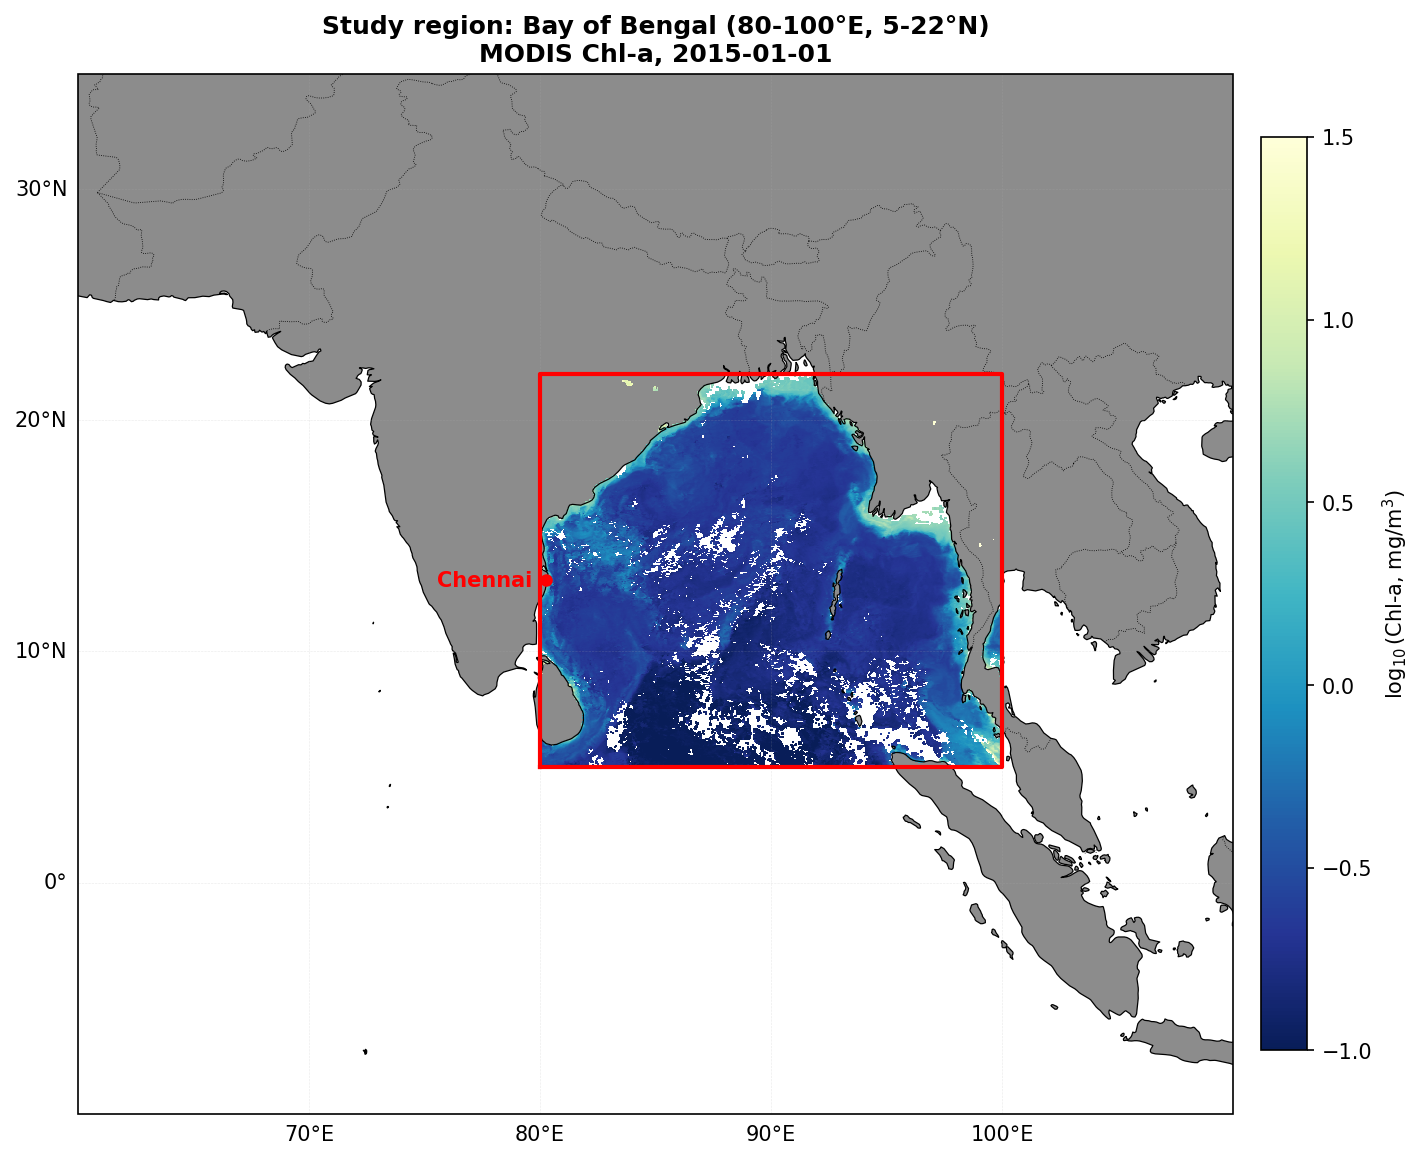
\includegraphics[width=\columnwidth]{Figures/study_region_context_map.png}
\caption{Wider geographic context for the Bay of Bengal study region
(60--110$^{\circ}$E, 10$^{\circ}$S--35$^{\circ}$N). Gray shows land.
White shows ocean outside the study domain, or ocean without a valid
retrieval on this date. Colour shows $\log_{10}$ Chl-a (mg/m$^3$)
from a representative MODIS composite (2017-01-01), shown only
inside the study domain (80--100$^{\circ}$E, 5--22$^{\circ}$N, red
box). Chennai is marked as a reference point.}
\label{fig:studyregion}
\end{figure}

Figure~\ref{fig:preprocessing} shows one representative composite,
in three stages of preprocessing: (a) the raw Chl-a field, (b) after
a $\log_{10}$ transform, and (c) after z-score normalization, with a
histogram below each panel. The raw distribution is strongly
right-skewed; the $\log_{10}$ transform makes it roughly symmetric.
Section~\ref{sec:pipeline} explains why this matters for the
reconstruction pipeline.

\begin{figure}[ht]
\centering
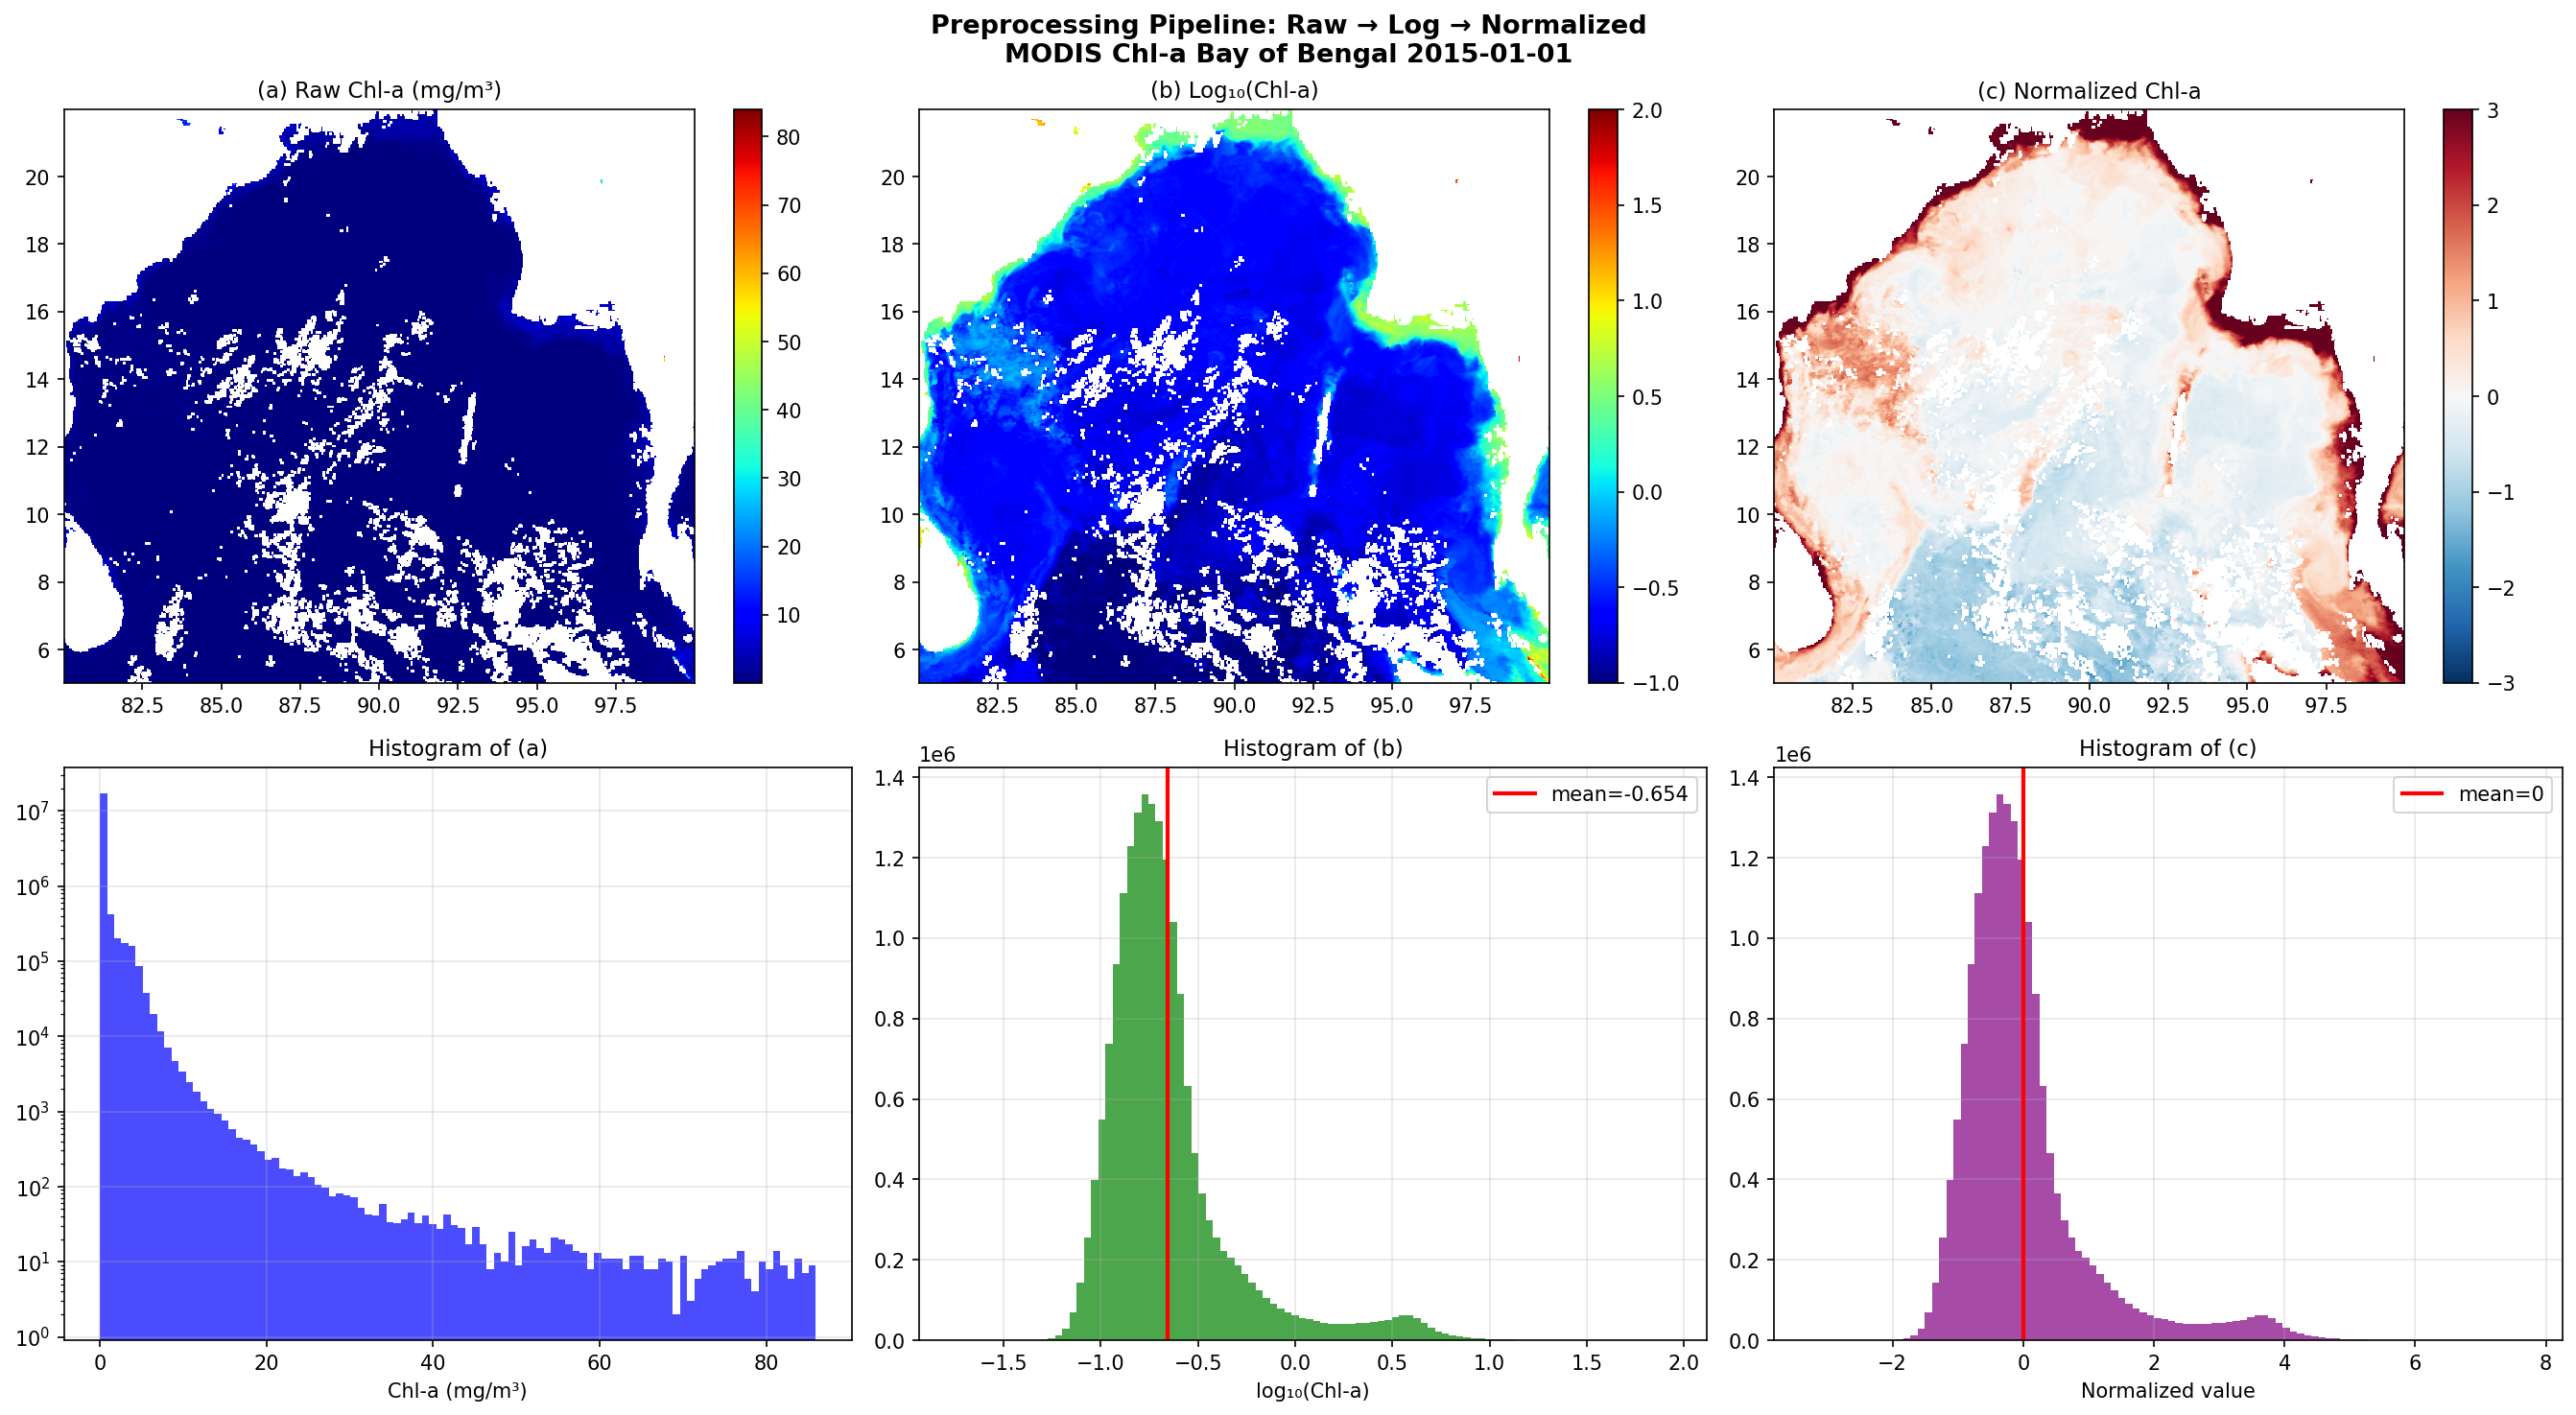
\includegraphics[width=\columnwidth]{Figures/chl_preprocessing.png}
\caption{Bay of Bengal study region shown via a representative MODIS
Chl-a composite (2015-01-01): (a) raw Chl-a concentration (mg/m$^3$)
and (b) after $\log_{10}$ transform, followed by (c) the field after
z-score normalization, with corresponding histograms of (a), (b), and
(c) shown below each panel.}
\label{fig:preprocessing}
\end{figure}

\subsection{Cell-NN data assimilation framework}

\subsubsection{Corrected relaxation equation}
\label{sec:relaxation}

We start with what the Cell-NN operator does, before writing its
equation. The operator holds a running estimate of the true state,
the relaxation variable $\mu_r$. At each moment it has access to an
observation $\mu_{obs}$. Its job is to pull $\mu_r$ toward
$\mu_{obs}$ smoothly, without letting one extreme observation
destabilize the estimate. This pull-and-limit behaviour is what the
equation below encodes.

The Cell-NN data assimilation operator updates $\mu_r$ toward
$\mu_{obs}$ according to
\begin{equation}
\frac{d\mu_r}{d\tau} = -(\mu_r - \mu_{obs}) + \alpha_A \cdot
\mathrm{clip}(\mu_{obs} - \mu_r,\, -1,\, 1),
\label{eq:relaxation}
\end{equation}
where $\tau$ is an internal relaxation time, separate from the
physical time of the underlying system, $\alpha_A$ is a single
scalar gain, and $\mathrm{clip}(x,-1,1) = \max(-1,\min(1,x))$ caps
its argument to $[-1,1]$.

Equation~\eqref{eq:relaxation} has two terms with different jobs.
The first, $-(\mu_r-\mu_{obs})$, is ordinary linear relaxation:
it always pulls $\mu_r$ toward $\mu_{obs}$ at a rate proportional
to the current gap. The second is the clip term. Without it, a
single large gap between $\mu_{obs}$ and $\mu_r$ could push the
correction to an arbitrarily large value and destabilize the
relaxation. The clip term prevents this, playing the same role as
the standard piecewise-linear output nonlinearity in the original
CeNN formulation \citep{chua1988theory}: it bounds a cell's
correction to a fixed range regardless of the discrepancy's size.
When $|\mu_{obs}-\mu_r|\leq 1$, it behaves linearly, giving smooth,
proportional correction near the fixed point. When
$|\mu_{obs}-\mu_r|>1$, it saturates at $\pm1$, so the correction
rate stops growing with the discrepancy. This produces the
two-regime behaviour formalized in Theorem~1: a bounded correction
far from the observation, exponential convergence close to it.

More generally, a CeNN template specifies a cell's local update via
three components: a coupling term $D$ relating each cell to its
neighbors, possibly nonlinear and time-varying; a linear coupling
term $C$; and a bias or forcing term $I$. Formally, for a network of
$K$ cells with state vector $\mathbf{X}(t) \in \mathbb{R}^K$, the
general CeNN template is
\begin{equation}
\dot{X}_k = -X_k + \sum_{j \in \mathcal{N}(k)} D_{k,j}(\mathbf{X},t)\, X_j
+ \sum_{j \in \mathcal{N}(k)} C_{k,j}\, X_j + I_k, \qquad k=1,\dots,K,
\label{eq:cenn_template}
\end{equation}
or in matrix form, $\dot{\mathbf{X}} = -\mathbf{X} +
D(\mathbf{X},t)\mathbf{X} + C\mathbf{X} + \mathbf{I}$, where
$\mathcal{N}(k)$ is the neighbor set of cell $k$, $D(\mathbf{X},t)
\in \mathbb{R}^{K\times K}$ is the nonlinear, time-varying coupling
matrix (zero outside $\mathcal{N}(k)$), $C \in \mathbb{R}^{K\times
K}$ is a fixed linear coupling matrix with the same sparsity
structure, and $\mathbf{I} \in \mathbb{R}^K$ is a per-cell bias
vector. The leading $-X_k$ term is the template's built-in unity
self-decay, which keeps the dynamics bounded independent of $D$,
$C$, and $I$.

At $K=3$, this template reduces to \citet{magno2025}'s own published
Lorenz-63 result (their Eqs.~7--8), small enough to write out in
full, which we reproduce here (independently re-verified by direct
substitution into Eq.~\eqref{eq:cenn_template}) as a concrete anchor
before generalizing to $K=40$. For state vector
$\boldsymbol{\mu}=[X,Y,Z]^\top$, reproducing the Lorenz-63 equations
$\dot{X}=\sigma(Y-X)$, $\dot{Y}=X(\rho-Z)-Y$, $\dot{Z}=XY-\beta Z$
requires no $A$- or $B$-type coupling,
\begin{equation}
A = \begin{pmatrix} 0&0&0\\0&0&0\\0&0&0\end{pmatrix}, \qquad
B = \begin{pmatrix} 0&0&0\\0&0&0\\0&0&0\end{pmatrix},
\label{eq:l63_AB}
\end{equation}
a fixed linear coupling matrix
\begin{equation}
C = \begin{pmatrix} 1-\sigma & \sigma & 0 \\ \rho & 0 & 0 \\ 0 & 0 & 1-\beta \end{pmatrix},
\label{eq:l63_C}
\end{equation}
and a nonlinear, time-varying coupling matrix carrying the two
quadratic terms $-XZ$ and $XY$,
\begin{equation}
D(t) = \begin{pmatrix} 0&0&0 \\ -Z(t)&0&0 \\ Y(t)&0&0 \end{pmatrix},
\label{eq:l63_D}
\end{equation}
with bias $\mathbf{I}=\mathbf{0}$. Row 1 of $C$ recovers
$\dot{X}=-X+(1-\sigma)X+\sigma Y=\sigma(Y-X)$; row 2 combines $C$'s
$\rho X$ term with $D$'s $-Z(t)\cdot X=-XZ$ term to recover
$\dot{Y}=-Y+\rho X-XZ=X(\rho-Z)-Y$; row 3 combines $C$'s $(1-\beta)Z$
term with $D$'s $Y(t)\cdot X=XY$ term to recover
$\dot{Z}=-Z+XY+(1-\beta)Z=XY-\beta Z$, confirming
Eqs.~\eqref{eq:l63_C}--\eqref{eq:l63_D} exactly reproduce the
Lorenz-63 system. Section~\ref{sec:l96template} casts the Lorenz-96
equation, Eq.~\eqref{eq:l96}, into this same template form at
$K=40$, deriving $D$, $C$, and $I$ explicitly; unlike this $3\times3$
case, a fully spelled-out $40\times40$ matrix is not practical to
display, so that derivation instead gives $D$'s exact sparsity
pattern and closed-form nonzero entries (Eq.~\eqref{eq:D_matrix}).

Equation~\eqref{eq:relaxation} is a corrected version of an earlier
formulation. \citet{magno2025} used a control template
$B^\text{DA}_{ij,kl}(\tau) = \mu^o_{ij}/(\mu^r_{ij}\,w_b)$, which
introduces a normalization parameter $w_b$ that biases the fixed
point. Integrating Eq.~\eqref{eq:relaxation} to convergence gives
$\mu_r^{\ast} = \mu_{obs}$ exactly, for any $\alpha_A$. We retain
$w_b$ for backward compatibility, though it does not appear in
Eq.~\eqref{eq:relaxation} and has no effect on the corrected fixed
point, confirmed both analytically and via a grid search over
$(\alpha_A, w_b)$ (Fig.~\ref{fig:sensitivity}), which shows results
invariant to $w_b$ for every tested $\alpha_A$. Parameter selection
therefore reduces to a one-dimensional search over $\alpha_A$; we
use the empirically optimal value $\alpha_A=1.0$ throughout unless
stated otherwise.

Following the matrix-template notation of \citet{magno2025} (their
Eqs.~14--16), the relaxation step can be written for the full state
vector $\boldsymbol{\mu}_r(\tau) \in \mathbb{R}^K$ as
\begin{equation}
\dot{\boldsymbol{\mu}}_r = -\boldsymbol{\mu}_r(\tau) +
A^\text{DA}\mathbf{v}(\tau) + B^\text{DA}\mathbf{u},
\label{eq:relaxation_matrix}
\end{equation}
with template matrices
\begin{equation}
A^\text{DA} = \alpha_A I_K, \qquad B^\text{DA} = I_K,
\label{eq:relaxation_AB}
\end{equation}
and per-cell activation and background terms
\begin{equation}
v_i(\tau) = \mathrm{clip}\bigl(\mu_{obs,i} - \mu_{r,i}(\tau),\, -1,\,
1\bigr), \qquad u_i = \mu_{obs,i},
\end{equation}
where $I_K$ is the $K\times K$ identity matrix. Both template
matrices are diagonal. This differs structurally from
\citet{magno2025}'s $B^\text{DA}$ (their Eq.~16), which couples each
cell to a spatial neighborhood through a ratio-based innovation term
with off-diagonal entries; the corrected relaxation step here has no
neighbor coupling of its own; $A^\text{DA}$ and $B^\text{DA}$ act
identically and independently on every cell. Cross-cell coupling
instead arises entirely from the nonlinear forecast between DA
cycles (Section~\ref{sec:cycle}), not from the relaxation step
itself.

Whether the operator performs true data assimilation, or simple
observation insertion, is not decided by the operator alone; it also
depends on the observation model. Our experiments indicate the
Cell-NN cycle performs genuine blending only when both of the
following hold.

\begin{enumerate}
\item \textbf{Noisy observations.} If the observation is effectively
noise-free, the operator converges toward the raw observation
regardless of the background. There is no uncertain information to
blend, only certain information to insert.
\item \textbf{A dynamically propagated background.} If the
background is simply the previous timestep's field, it carries no
independent forecast information. Without real tension between
background and observation, the update is not a meaningful
assimilation step.
\end{enumerate}

At each relaxation step, the operator converges closely to
$\mu_{obs}$ regardless of which condition holds;
Section~\ref{sec:results} confirms this for Lorenz-96. What actually
separates the two regimes is not how completely a single step
converges. Section~\ref{sec:cycle} gives this mechanism its own
treatment, since it is the one genuinely non-obvious idea in this
framework: blending emerges between correction cycles, not within
any single relaxation step.

%% ---- CONVERGENCE THEOREM -----------------
\medskip
\noindent\textbf{Theorem~1 (Convergence of the Cell-NN relaxation).}
\textit{Let $\mu_r(\tau)$ satisfy Eq.~\eqref{eq:relaxation} with
$\alpha_A > 0$ and fixed $\mu_{obs}$. Define the tracking error
$e(\tau) = \mu_r(\tau) - \mu_{obs}$. Then:}
\begin{enumerate}
\item[(i)] \textit{The unique fixed point is $\mu_r^{\ast} = \mu_{obs}$,
so $e(\tau) \to 0$ as $\tau \to \infty$.}
\item[(ii)] \textit{When $|e(\tau)| \leq 1$, convergence is exponential:}
\begin{equation}
|e(\tau)| \;\leq\; |e(0)|\,\exp\!\bigl(-(1+\alpha_A)\,\tau\bigr).
\label{eq:convergence_rate}
\end{equation}
\item[(iii)] \textit{When $|e(\tau)| > 1$, the error satisfies
$\dot{e} = -e - \alpha_A\,\mathrm{sgn}(e)$. This adds a constant pull
of magnitude $\alpha_A$ on top of the bare linear term $-e$, so
$|e(\tau)|$ reaches the boundary $|e|=1$ in finite pseudo-time, after
which part (ii) applies.}
\end{enumerate}

\noindent\textit{Proof sketch.}
Part (i): evaluating the right-hand side of
Eq.~\eqref{eq:relaxation} at $\mu_r=\mu_{obs}$ gives
$-(\mu_{obs}-\mu_{obs}) + \alpha_A\cdot\mathrm{clip}(0,-1,1) = 0$,
so $\mu_{obs}$ satisfies $f(\mu_r^{\ast})=\mu_r^{\ast}$. Uniqueness
follows because the right-hand side is strictly decreasing in
$\mu_r$: the sum of a strictly decreasing linear term and a
non-increasing clip term can have at most one root. Substituting
$e(\tau) = \mu_r(\tau) - \mu_{obs}$ gives $\dot{e} = -e -
\alpha_A\,\mathrm{clip}(e,-1,1)$, using
$\mathrm{clip}(\mu_{obs}-\mu_r,-1,1) = \mathrm{clip}(-e,-1,1) =
-\mathrm{clip}(e,-1,1)$, from the odd symmetry of clip about zero.

Part (ii): in the linear regime ($|e| \leq 1$),
$\mathrm{clip}(e,-1,1) = e$, so $\dot{e} = -(1+\alpha_A)\,e$, which
integrates to $e(\tau) = e(0)\exp(-(1+\alpha_A)\tau)$: exponential
decay with rate $(1+\alpha_A)$.

Part (iii): in the saturated regime ($|e|>1$),
$\mathrm{clip}(e,-1,1)=\mathrm{sgn}(e)$, so $\dot{e} = -e -
\alpha_A\,\mathrm{sgn}(e) = -(|e|+\alpha_A)\,\mathrm{sgn}(e)$. This
magnitude, $|e|+\alpha_A$, exceeds the bare linear term $|e|$ alone
by the fixed amount $\alpha_A$, for every $\alpha_A>0$ and every
$|e|>1$; that is, the saturated correction is strictly larger than
what unmodified linear relaxation ($\dot e=-e$) would give at the
same $|e|$, not a claim about the rate coefficient in part (ii). This
guarantees $|e|$ reaches the linear-regime boundary in finite
pseudo-time, unlike bare exponential decay, which approaches any
threshold only asymptotically. $\square$

\noindent\textbf{Corollary (effect of $\alpha_A$ on convergence
rate).} The exponential decay rate $\lambda = -(1+\alpha_A)$
increases linearly with $\alpha_A$, agreeing with the empirical
result that $\alpha_A=1.0$, doubling the decay rate relative to
$\alpha_A=0$, outperforms smaller values in the parameter grid
search. For $\alpha_A=1.0$ and step size $\Delta\tau =
5\times10^{-2}$, the theoretical per-step reduction factor is
$\exp(-2\Delta\tau) \approx 0.905$. If the iteration cap
$r_\text{max}=50$ were reached in the linear regime, the residual
error would be about $0.7\%$ of its initial value. In practice,
under the fixed pseudo-time budget used throughout this study,
$r_\text{max}=50$ is reached at every DA cycle before the tolerance
$\epsilon_\text{conv}$ is met; as Section~\ref{sec:results} shows,
the residual is still small relative to the state magnitude.
%% ---- END CONVERGENCE THEOREM ----------------------------------------

Global stability was also verified via a Lyapunov analysis for both
Lorenz-63 and Lorenz-96 (Figure~\ref{fig:lyapunov}). Panels (a)-(b)
show the Lyapunov function decaying monotonically for Lorenz-63;
panels (c)-(d) repeat this for Lorenz-96. Together they confirm
asymptotic stability independently of Theorem~1's scalar proof.

\begin{figure}[ht]
\centering
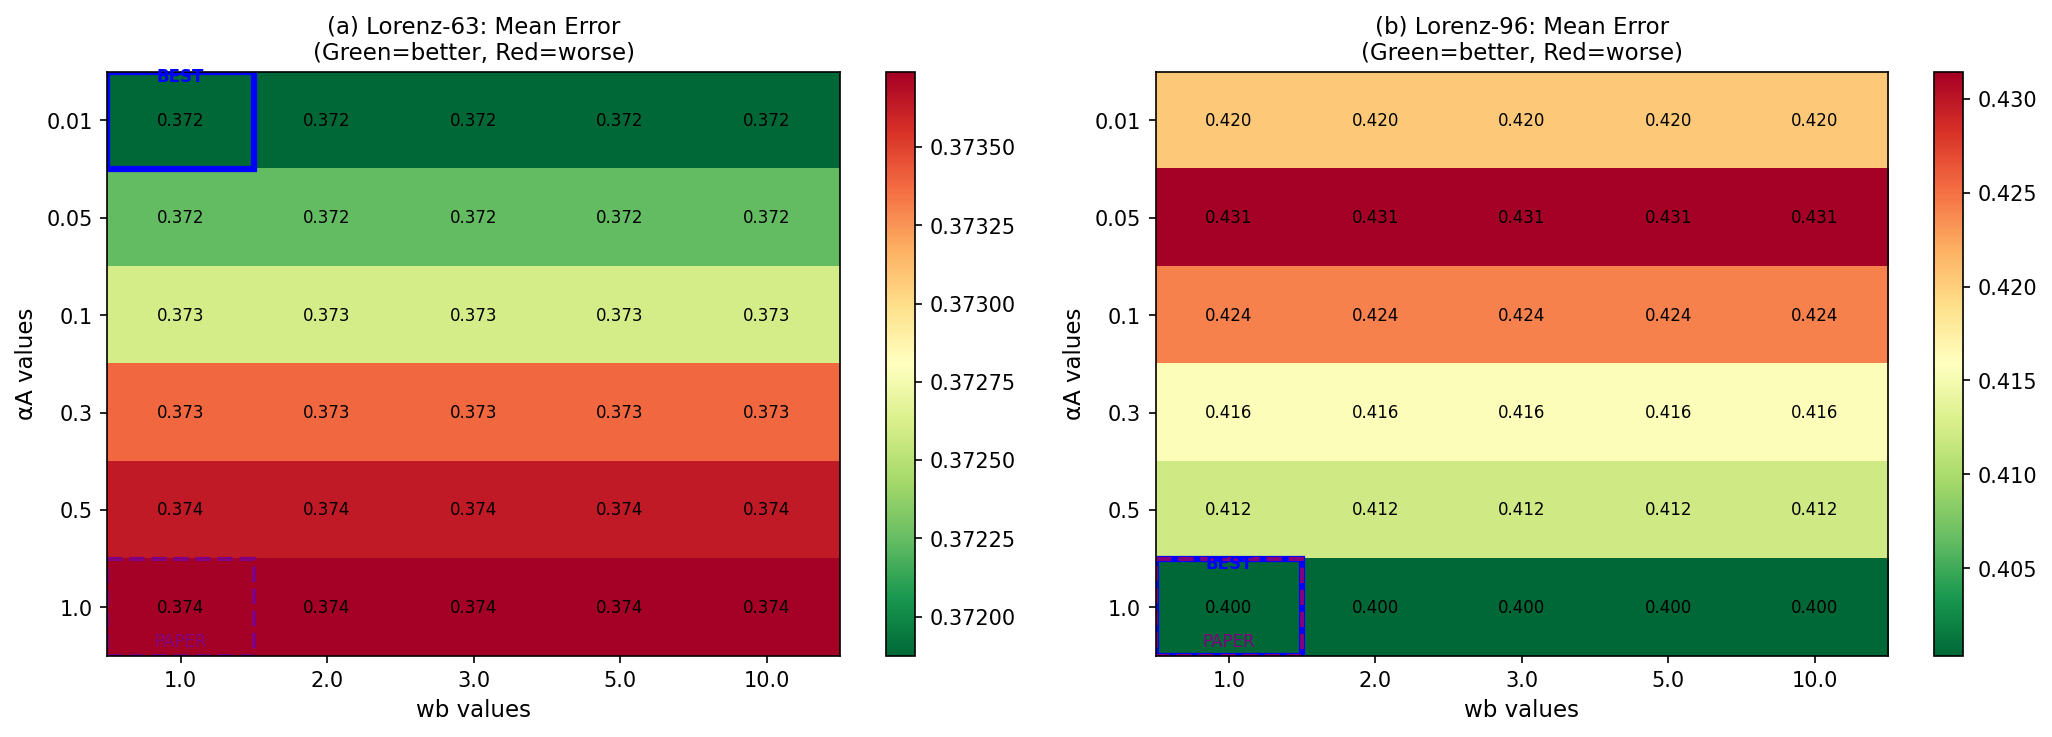
\includegraphics[width=\columnwidth]{Figures/template_sensitivity.png}
\caption{\large Grid search over $\alpha_A$ and $w_b$: (a) Lorenz-63 and
(b) Lorenz-96 mean error. Results are invariant to $w_b$ for every
tested $\alpha_A$.}
\label{fig:sensitivity}
\end{figure}

\begin{figure}[ht]
\centering
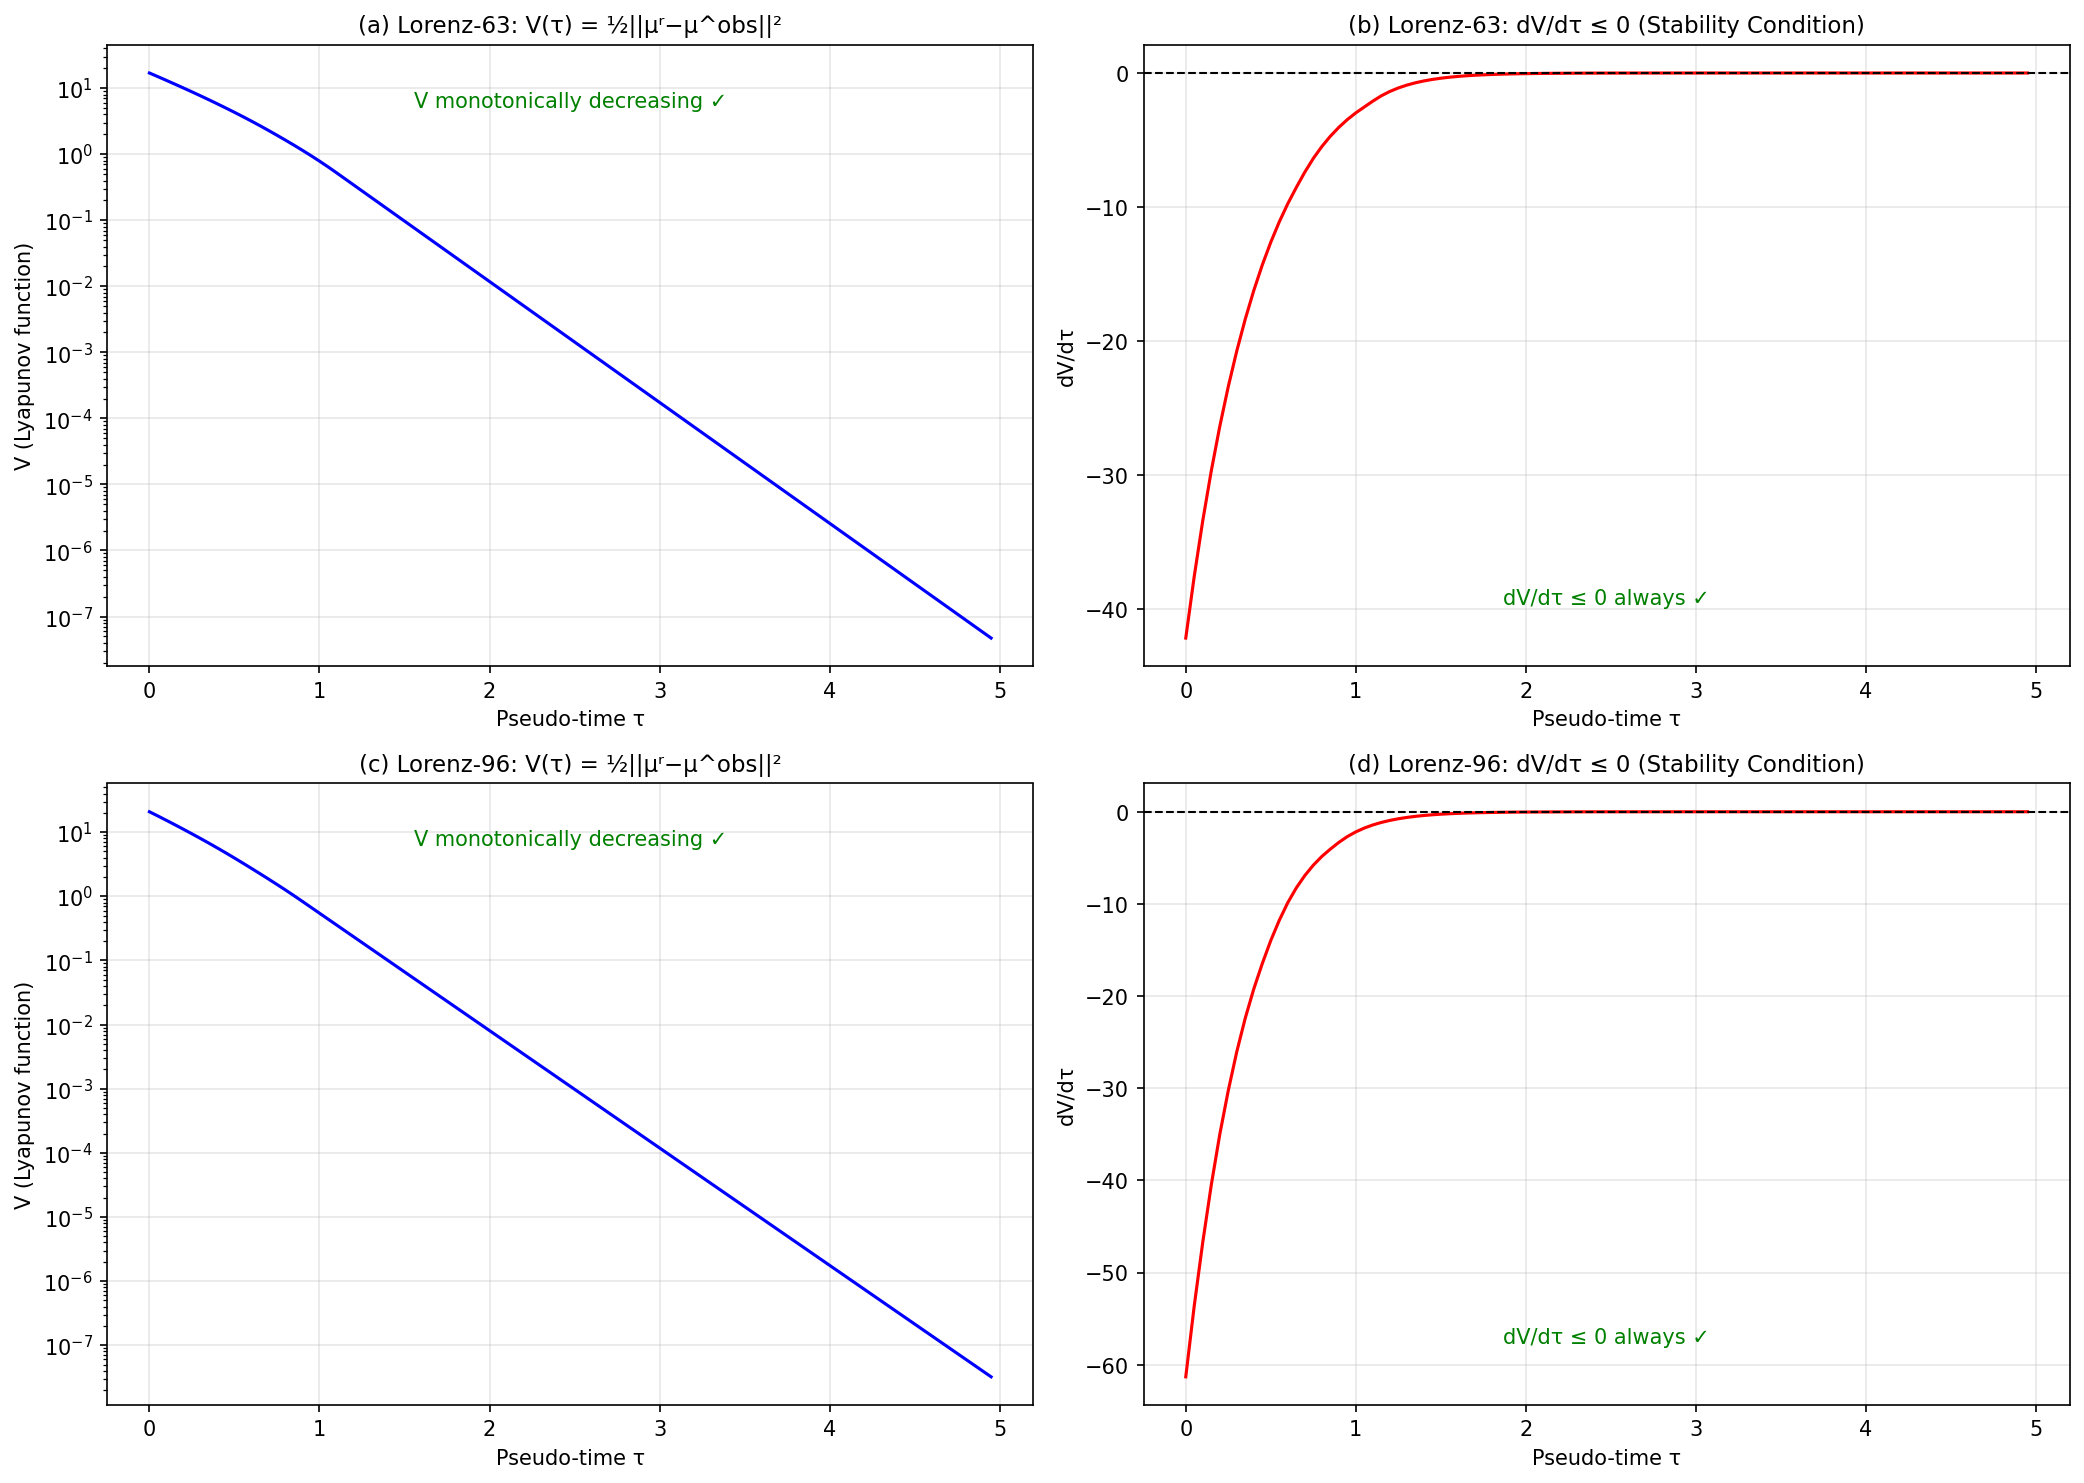
\includegraphics[width=\columnwidth]{Figures/lyapunov_stability.png}
\caption{Lyapunov stability verification of the Cell-NN DA scheme.
Panels (a) and (b) show the Lyapunov function analysis for the
Lorenz-63 system: (a) the Lyapunov function
$V(\tau)=\tfrac{1}{2}\|\mu^r-\mu^{obs}\|^2$ decaying monotonically
with pseudo-time $\tau$, and (b) the stability condition $dV/d\tau
\leq 0$, confirming asymptotic stability. Panels (c) and (d) show the
same analysis for Lorenz-96.}
\label{fig:lyapunov}
\end{figure}

\subsubsection{Cycle-level propagation: how blending actually emerges}
\label{sec:cycle}

Theorem~1 establishes what happens within a single relaxation step:
convergence toward $\mu_{obs}$, bounded and exponential once close
enough. That result alone does not explain the two-condition
diagnostic, since a single step converges closely to $\mu_{obs}$
regardless of which condition holds. The mechanism that actually
separates genuine assimilation from observation insertion operates
one level up, between correction cycles, not within any one of them.

Three steps repeat every DA cycle. First, the relaxation step
(Eq.~\eqref{eq:relaxation}) corrects the currently observed
variables toward the current observation; unobserved variables are
untouched by this step. Second, the nonlinear forecast that runs
between cycles propagates this correction through the system's
coupled dynamics, carrying it from the variables that were just
corrected to the variables that were not. Third, the resulting
state, now bearing the propagated correction, becomes the background
for the next cycle, so the correction persists rather than being
overwritten at the next step.

When both conditions of Section~\ref{sec:relaxation} hold, all three
steps are active. The forecast in step two is a real, dynamically
propagated model, so it genuinely carries information from observed
to unobserved variables; repeating this cycle after cycle is what
constitutes true blending, at the level of the full assimilation
cycle rather than any single relaxation step. When neither condition
holds, step two has no equivalent: a persistence background is
simply the previous field, so there is no forecast to carry a
correction anywhere. Step three then adds nothing beyond what step
one already did at the currently observed pixels; the next
background is unchanged elsewhere. Coupling never emerges, no matter
how many cycles run, because the one step responsible for
propagating it is absent. Sections~\ref{sec:attribution}
and~\ref{sec:rectmask} support this experimentally, for the satellite
setting, where step two is genuinely missing.

Both conditions can be checked directly from the observation model,
before any experiment is run: is the background produced by a
forecast (step two exists), and are the observations noisy (step one
has real uncertainty to blend, not just a certain value to insert)?
Sections~\ref{sec:results} and~\ref{sec:discussion} test this
prediction in two domains that answer these two questions oppositely:
Lorenz-96, where both conditions hold, and direct satellite
retrieval, where neither does.

\subsubsection{Lorenz-63 reproduction}

Before extending to a higher-dimensional system, we reproduce the
original Lorenz-63 result as a sanity check: does the corrected
relaxation equation still behave as expected on the system it was
originally validated on? We reproduced the Cell-NN result of
\citet{magno2025} on Lorenz-63 \citep{lorenz1963}, using
Eq.~\eqref{eq:relaxation} in place of the original, uncorrected
equation, with matched noise level, observation interval, and
DA-on/off scheduling. Figure~\ref{fig:lorenz63} compares the true
trajectory against the background (no-assimilation) trajectory for
$X(t)$, $Y(t)$, $Z(t)$; the background visibly diverges once chaotic
dynamics amplify the initial perturbation, which is exactly why data
assimilation is needed.

\begin{figure}[ht]
\centering
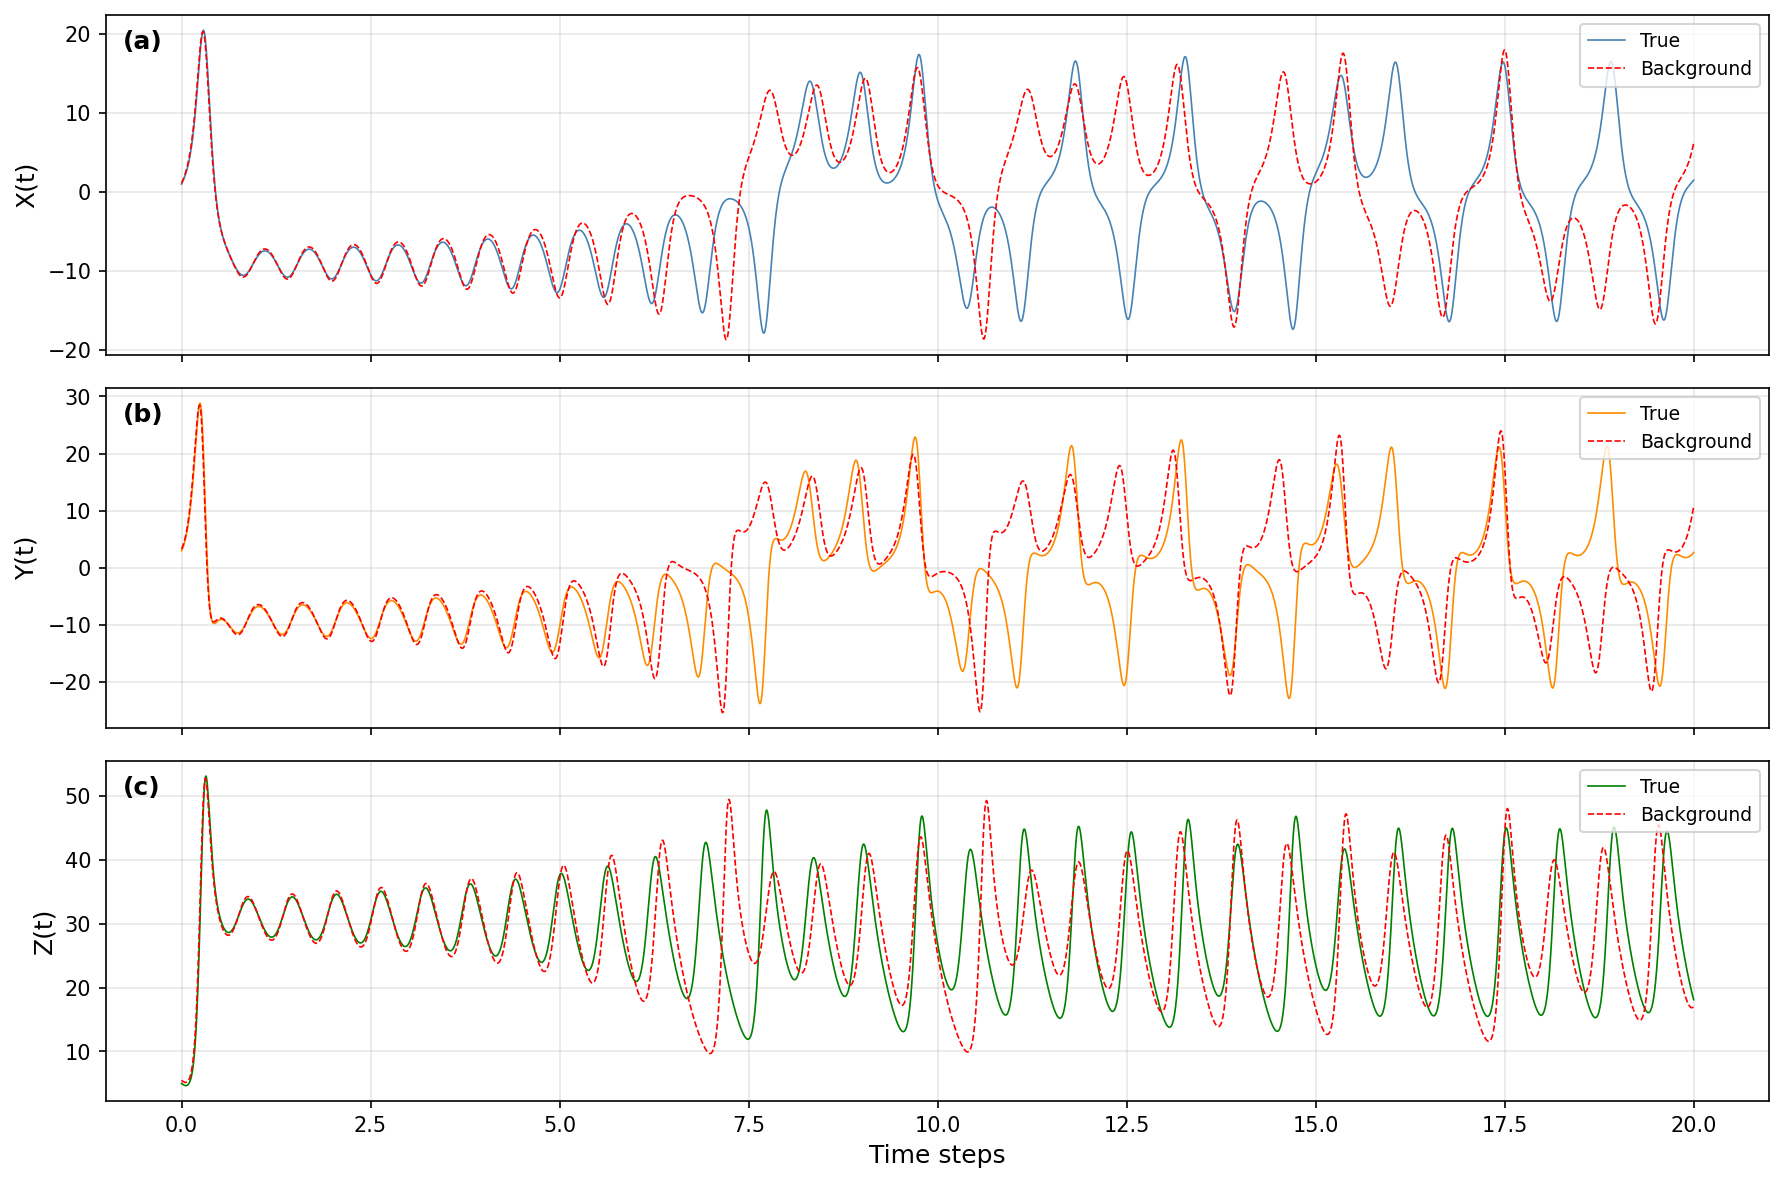
\includegraphics[width=\columnwidth]{Figures/lorenz63_trajectory.png}
\caption{Lorenz-63 trajectories, true state versus background: (a)
$X(t)$, (b) $Y(t)$, (c) $Z(t)$, reproducing \citet{magno2025}.}
\label{fig:lorenz63}
\end{figure}

\subsubsection{Lorenz-96 extension and template derivation}
\label{sec:l96template}

The Lorenz-96 system is a chaotic system of $K$ coupled
variables arranged in a ring, each interacting only with its near
neighbors, yet exhibiting complex, unpredictable dynamics as a whole.
It is a standard data-assimilation benchmark precisely because it is
higher-dimensional than Lorenz-63, while still cheap to simulate.

The Lorenz-96 system \citep{lorenz1998} is defined, for
$k=1,\dots,K$ (cyclic), by
\begin{equation}
\frac{dX_k}{dt} = (X_{k+1}-X_{k-2})X_{k-1} - X_k + F,
\label{eq:l96}
\end{equation}
with constant forcing $F$. The forcing pushes energy in continuously;
the linear damping term $-X_k$ removes energy, keeping the system
bounded; the remaining term, $(X_{k+1}-X_{k-2})X_{k-1}$, couples each
variable to its neighbors and is the source of the chaotic behaviour.

We now derive how Eq.~\eqref{eq:l96} maps onto the general CeNN
template, Eq.~\eqref{eq:cenn_template}: matching term by term to
identify $D$, $C$, and $I$ for this specific system, on top of the
template's built-in unity self-decay.

\textbf{Self-decay term.} Every Cell-NN cell carries an intrinsic
self-decay of $-X_k$, keeping the dynamics bounded regardless of the
applied template. Lorenz-96's own damping term, $-X_k$, has exactly
this form and needs no separate fitting.

\textbf{Bias term.} The forcing $F$ is constant across every cell
and time step, matching the Cell-NN bias term directly: $I=F$.

\textbf{Coupling term.} The remaining term,
$(X_{k+1}-X_{k-2})X_{k-1}$, couples cell $k$ to its neighbors at
$k-1$, $k+1$, $k-2$. Writing it as a coefficient on $X_{k-1}$,
\begin{equation}
(X_{k+1}-X_{k-2})\,X_{k-1} = D_{k,k-1}(t)\cdot X_{k-1}, \qquad
D_{k,k-1}(t) = X_{k+1}(t) - X_{k-2}(t).
\end{equation}
This coefficient depends on two other state variables, so it changes
with time, unlike the fixed coefficients typical of standard Cell-NN
image-processing templates. We classify it as the nonlinear,
time-varying $D$-type coupling term rather than the constant-coefficient
$C$-type term; no further $C$-type coupling is needed, so $C=0$.

In the explicit matrix notation of Eq.~\eqref{eq:cenn_template},
paralleling \citet{magno2025}'s Eqs.~7--8 for Lorenz-63, the linear
coupling matrix is the zero matrix, $C = \mathbf{0}_{K\times K}$, and
the nonlinear coupling matrix $D(\mathbf{X},t) \in \mathbb{R}^{K
\times K}$ has exactly one nonzero entry per row, in column $k-1$:
row $k$ of $D(\mathbf{X},t)$ is
\begin{equation}
\bigl(D_{k,1},\, \ldots,\, D_{k,k-2},\, D_{k,k-1},\, D_{k,k},\,
\ldots,\, D_{k,K}\bigr) = \bigl(0,\, \ldots,\, 0,\, X_{k+1}(t) -
X_{k-2}(t),\, 0,\, \ldots,\, 0\bigr),
\label{eq:D_matrix}
\end{equation}
for $k=1,\dots,K$ (indices cyclic). Unlike the $3\times3$ Lorenz-63
case, where \citet{magno2025} write out every entry of $C$ and $D$
explicitly (their Eqs.~7--8), Lorenz-96's $K=40$ dimensionality makes
a fully spelled-out $40\times40$ matrix impractical to display;
Eq.~\eqref{eq:D_matrix} instead gives the matrix's exact sparsity
pattern and the closed-form value of its one nonzero entry per row,
which together fully specify $D(\mathbf{X},t)$.

Putting the three components together,
\begin{equation}
\frac{dX_k}{dt} = \underbrace{-X_k}_{\text{self-decay}} +
\underbrace{D_{k,k-1}(t)\,X_{k-1}}_{\text{coupling}} +
\underbrace{C}_{=0} + \underbrace{I}_{=F},
\end{equation}
reproduces Eq.~\eqref{eq:l96} exactly. We verified this numerically:
integrating the Cell-NN template with $D$, $C$, $I$ as above and
comparing against RK45 applied directly to Eq.~\eqref{eq:l96} agree
to within about $10^{-13}$, reported as the ODE-score
(Table~\ref{tab:lorenz_results}) and defined precisely in
Section~\ref{sec:metrics}.

\subsubsection{Baseline methods}
\label{sec:baselines}

We compare Cell-NN against three established baselines, plus a
stronger EnKF variant introduced in Section~\ref{sec:robustness}.

\textbf{(a) 3D-Var.} A standard variational analysis with a fixed
background-error covariance. The classical, training-free baseline
used throughout. The analysis minimizes the cost function
\begin{equation}
J(\mathbf{w}) = \frac{1}{2}(\mathbf{w}-\mathbf{w}_b)^\top
\mathbf{B}^{-1} (\mathbf{w}-\mathbf{w}_b) +
\frac{1}{2}(H\mathbf{w}-\mathbf{y})^\top \mathbf{R}^{-1}
(H\mathbf{w}-\mathbf{y}),
\label{eq:3dvar_cost}
\end{equation}
where $\mathbf{w}_b$ is the background, $\mathbf{y}$ the observation
vector, and $H$ the observation operator, a matrix picking out the
observed state entries. The minimizer has the closed form
\begin{equation}
\mathbf{w}_a = \mathbf{w}_b + \mathbf{K}(\mathbf{y} - H\mathbf{w}_b),
\qquad
\mathbf{K} = \left(\mathbf{B}^{-1} + H^\top \mathbf{R}^{-1}
H\right)^{-1} H^\top \mathbf{R}^{-1},
\label{eq:3dvar_gain}
\end{equation}
the information-form Kalman gain, used directly in our
implementation. Both the background-error covariance $\mathbf{B}$
and observation-error covariance $\mathbf{R}$ are diagonal and
isotropic, $\mathbf{B}=\sigma_b^2 I$, $\mathbf{R}=\sigma_r^2 I$. The
values used in Table~\ref{tab:lorenz_results}, $\sigma_b=0.5$,
$\sigma_r=0.1$, are standard, reasonable defaults; unlike Cell-NN's
$\alpha_A$, chosen by an explicit grid search with confirmed
invariance to $w_b$ (Figure~\ref{fig:sensitivity}), they were not
originally swept. We closed this asymmetry directly: a $5\times5$
grid search over $\sigma_b \in \{0.1, 0.3, 0.5, 0.7, 1.0\}$ and
$\sigma_r \in \{0.05, 0.1, 0.2, 0.3, 0.5\}$
(Table~\ref{tab:threedvar_sensitivity}), using the same intermittency
schedule and R-score convention as Table~\ref{tab:lorenz_results}.
The default point reproduces R-score$=1.411$ exactly, confirming the
grid is consistent with the main comparison. The best point in the
grid, $\sigma_b=0.7$, $\sigma_r=0.05$, reaches R-score$=1.374$, still
worse than Cell-NN's irregular-observation R-score of $1.245$, a
9.4\% gap against the best-tuned 3D-Var found here, larger than the
3.7\% average improvement reported across 20 realizations against the
original, untuned baseline; these two percentages are not the same
comparison; one is a single realization against the best grid point,
the other an average across realizations against the default point,
and should not be conflated. The best point sits at the edge of the
tested range for $\sigma_r$, so a still-lower value might improve
3D-Var further; we did not widen the grid beyond this range, the same
caveat already applied to the diffusion and OI grids
(Section~\ref{sec:limitations}).

\begin{table}[t]
\centering
\small
\caption{3D-Var covariance sensitivity: R-score under the
intermittency schedule (DA-on 0--2000, off 2000--3500, on
3500--5000), same protocol as Table~\ref{tab:lorenz_results}.
Default ($\sigma_b=0.5$, $\sigma_r=0.1$, $\dag$) reproduces
R-score$=1.411$ exactly; best in grid ($\sigma_b=0.7$,
$\sigma_r=0.05$, $\ast$) reaches $1.374$, still above Cell-NN's
$1.245$.}
\label{tab:threedvar_sensitivity}
\begin{tabular}{lccccc}
\toprule
 & \multicolumn{5}{c}{$\sigma_r$} \\
\cmidrule(lr){2-6}
$\sigma_b$ & 0.05 & 0.10 & 0.20 & 0.30 & 0.50 \\
\midrule
0.1 & 2.631 & 7.317 & 17.102 & 21.693 & 24.645 \\
0.3 & 1.499 & 1.835 & 2.653 & 7.506 & 14.528 \\
0.5 & 1.543 & 1.411$^\dag$ & 1.726 & 2.683 & 7.317 \\
0.7 & \textbf{1.374}$^\ast$ & 1.534 & 1.857 & 2.071 & 4.452 \\
1.0 & 1.406 & 1.543 & 1.411 & 1.906 & 2.633 \\
\bottomrule
\end{tabular}
\end{table}

\textbf{(b) EnKF.} An ensemble Kalman filter with Gaspari-Cohn
localization, under two observation regimes: continuous (every DA
cycle observed) and irregular (observations switch on and off in
blocks), testing sensitivity to gappy availability. Given an
$N_\text{ens}$-member ensemble $\{\mathbf{x}^{(m)}\}_{m=1}^{N_\text{ens}}$
with mean $\bar{\mathbf{x}}$, inflated perturbations
$\mathbf{x}^{(m)} \to \bar{\mathbf{x}} + \lambda(\mathbf{x}^{(m)} -
\bar{\mathbf{x}})$ for inflation factor $\lambda$, the forecast
covariance is estimated as
\begin{equation}
P_f = \frac{1}{N_\text{ens}-1} \sum_{m=1}^{N_\text{ens}}
(\mathbf{x}^{(m)}-\bar{\mathbf{x}})(\mathbf{x}^{(m)}-\bar{\mathbf{x}})^\top.
\label{eq:enkf_cov}
\end{equation}
Each member is updated with perturbed observations, the standard
stochastic EnKF formulation:
\begin{equation}
\mathbf{x}_a^{(m)} = \mathbf{x}^{(m)} + \mathbf{K}\left(\mathbf{y} +
\boldsymbol{\epsilon}^{(m)} - H\mathbf{x}^{(m)}\right), \qquad
\boldsymbol{\epsilon}^{(m)} \sim \mathcal{N}(0,\mathbf{R}),
\label{eq:enkf_update}
\end{equation}
\begin{equation}
\mathbf{K} = \bigl(\rho \circ P_f H^\top\bigr)
\left(HP_fH^\top + \mathbf{R}\right)^{-1},
\label{eq:enkf_gain}
\end{equation}
where $\rho$ is the Gaspari-Cohn localization function, applied by
elementwise (Schur) product to $P_f H^\top$, localizing the gain
directly rather than the full covariance matrix. We also test a
relaxation-to-prior-spread (RTPS) adaptive-inflation variant
\citep{whitaker2012rtps}, which estimates inflation from the
ensemble's own spread each cycle instead of a fixed, hand-swept
constant; results are reported in Section~\ref{sec:robustness}.

\textbf{(c) 4DVarNet.} The learned variational solver of
\citet{fablet2021}, trained on 200-step patches of the Lorenz-96
trajectory (20 epochs, batch size 16, Adam, learning rate
$10^{-3}$). We report this comparison with an explicit caveat:
4DVarNet needs a large training dataset with ground truth, while
3D-Var and Cell-NN do not; we treat the comparison as informative
about where Cell-NN sits relative to the trained end of the
spectrum, not as a like-for-like contest.

\subsubsection{Diagnostics}
\label{sec:diagnostics}

We report two diagnostics for the Lorenz systems, following the
conventions of \citet{fablet2021}: the R-score and the ODE-score,
both defined precisely in Section~\ref{sec:metrics}. Briefly, the
R-score is the mean squared error during DA-on intervals only,
excluding free-running drift; an earlier implementation included
drift periods and underestimated divergence under irregular
observations. The ODE-score is the one-step-ahead prediction error
under RK4 integration; an earlier Euler-based implementation
overstated integration error by roughly six orders of magnitude
($4.26\times10^{-7}$ versus the corrected $1.79\times10^{-13}$).

\subsubsection{Advantages of relaxation-based methods}
\label{sec:nudging}

The Cell-NN operator belongs to the family of relaxation-based
correction schemes. Newtonian nudging, or spectral nudging, adds a
relaxation term $\alpha(\mathbf{x}_{obs} - \mathbf{x})$ to the
model's tendency equation, with $\alpha$ a spatially uniform
coefficient \citep{kalnay2003}. Cell-NN generalizes this two ways:
the relaxation runs iteratively in a pseudo-time $\tau$ separate
from physical time, allowing several internal correction steps per
DA cycle; and the clip function adds a nonlinear saturation that
prevents overcorrection.

To be explicit about what this operator is not: it is not a Bayesian
method, not a variational method, and not an optimal estimator in
any formal sense. It specifies no error covariance, computes no
posterior distribution, and does not minimize an explicit cost
function. It is a relaxation operator with a bounded correction rule,
and its guarantees follow from that identity, not from an implicit
approximation to a Bayesian update. Direct observation insertion
corresponds to full convergence of the relaxation step to the
observation; in the satellite application, the relaxation step uses
the full iteration budget at every DA cycle
(Section~\ref{sec:results}), reaching a residual small relative to
the normalized state magnitude.

Incremental 3D-Var differs fundamentally: it introduces a
background-error covariance $\mathbf{B}$ that explicitly weights
background against observation. Cell-NN uses no such matrix, and
needs no specification of $\mathbf{B}$; this is both its key
practical advantage, training-free and covariance-free, and the
reason it cannot weight background and observation optimally in a
Bayesian sense. Table~\ref{tab:cost} summarizes the computational and
parametric differences between all methods.

\subsection{Preprocessing}

We apply the identical Cell-NN operator (Eq.~\eqref{eq:relaxation},
$\alpha_A=1.0$) to the Aqua-MODIS Chl-a composites, with no
retraining and no change to the governing equation. Only the spatial
adjacency template differs from the Lorenz-96 case, since the
satellite data live on a 2-D image domain rather than a 1-D cyclic
lattice.

Chl-a concentrations follow a strongly right-skewed, approximately
log-normal distribution \citep{campbell1995}. We apply a $\log_{10}$
transform followed by z-score normalization. MODIS and the L4
reference are normalized independently, each with its own mean and
standard deviation (MODIS: $\mu=-0.654$, $\sigma=0.336$; L4:
$\mu=-0.672$, $\sigma=0.332$), preserving rather than removing the
0.018 difference between the two products' mean log-Chl-a, which may
reflect a genuine physical difference or a residual calibration
offset. Figure~\ref{fig:preprocessing} shows the effect of this
transform chain.

\paragraph{Cell-NN-guided reconstruction pipeline}
\label{sec:pipeline}

For each 8-day composite at time $t$, the background is the previous
composite, $\mu_b = X(t-1)$. Cell-NN relaxation is applied only to
pixels with a valid observation at time $t$; cloud gaps are not
updated by the Cell-NN equation at all, instead filled by 50
iterations of Laplacian spatial diffusion from neighboring pixels,
$\kappa=0.4$.

Choosing these two numbers needs care, to avoid a subtle statistical
mistake: picking them by testing combinations against the same
held-out pixels later used to report performance would make the
reported number mildly optimistic. To avoid this, the internal 20\%
held-out set (below) is split into two disjoint halves with an
independent random seed: a 10\% validation subset and a 10\% test
subset. Diffusion hyperparameters were chosen by a $4\times4$ grid
search over $\kappa \in \{0.1, 0.2, 0.3, 0.4\}$ and iteration count
$\in \{10, 20, 30, 50\}$, evaluated on the validation subset only
(Table~\ref{tab:diff_sensitivity}); every other result, including
Table~\ref{tab:chl_validation}, is reported on the disjoint test
subset, which plays no role in hyperparameter selection.

We call the combined Cell-NN and diffusion procedure the
reconstruction pipeline. A controlled ablation
(Section~\ref{sec:attribution}) shows that reconstruction skill at
currently unobserved pixels comes from the diffusion component, not
Cell-NN, whose role in this noise-free setting is limited to
correcting currently observed pixels. Diffusion plays the same
structural role here that the nonlinear forecast plays in Lorenz-96
(Section~\ref{sec:relaxation}): propagating a correction from
observed to unobserved locations, which the persistence background
cannot do on its own.

\paragraph{DINEOF baseline}

As a standard reference, we implement DINEOF (Data Interpolating
Empirical Orthogonal Functions) \citep{beckers2003dineof} from
scratch, cross-validated against the original MATLAB code and the
\texttt{py-DINEOF} library. The algorithm alternates filling missing
values with the current low-rank reconstruction and updating the
truncated SVD, keeping the $r$ leading EOF modes. Optimal $r$ is
chosen by cross-validation on 2\% of observed pixels, withheld
separately from the main 20\% held-out set; RMSE decreases
monotonically before plateauing at $r=17$ EOFs (CV-RMSE=0.385) and
rising slightly at $r=19$--$20$, consistent with published DINEOF
behaviour \citep{beckers2003dineof,alvera2005}.

\paragraph{Optimal Interpolation baseline}

As a second classical baseline, we implement Optimal Interpolation
(OI) \citep{bretherton1976} with a Gaussian spatial covariance
kernel, $C(\mathbf{x}_i, \mathbf{x}_j) = \exp(-|\mathbf{x}_i -
\mathbf{x}_j|^2 / 2L^2)$, where $L$ is optimized by leave-one-out
cross-validation on the validation subset, using the same
10-timestep subset as DINEOF. All five gap-filling methods are
evaluated on identical held-out test pixels.

\paragraph{Hyperparameter selection and leakage, summarized}

Three methods in this comparison have a hyperparameter chosen from
data: Cell-NN's $\kappa$ and iteration count, DINEOF's $r$, and OI's
$L$. All three are selected without touching the test subset used
for final reporting, though by two different routes. Cell-NN's
$\kappa$ and iteration count, and OI's $L$, are both chosen on the
same validation subset (Section~\ref{sec:pipeline}), disjoint from
the test subset. DINEOF's $r$ is chosen on a separate 2\%
cross-validation subset, disjoint from the main 20\% held-out set
entirely, so its selection is independent of the val/test split by
construction, not merely restricted to one half of it. In every
case, only final scoring, not hyperparameter selection, uses the
test subset. Monte Carlo and the persistence background have no
tunable hyperparameters, so this distinction does not apply to them.

\paragraph{Validation protocol}

\textbf{Internal (random mask-and-recover).} At each timestep, 20\%
of currently valid pixels are withheld, with a fixed random seed
whose stream continues across timesteps. This 20\% is split into two
disjoint 10\% halves with an independent seed: a validation subset
used only to select diffusion hyperparameters
(Section~\ref{sec:pipeline}), and a test subset used for every other
reported result. No pixel is ever used both to select hyperparameters
and to report performance against them.

\textbf{Cloud-shaped masking.} Real cloud gaps are contiguous, not
scattered like random masking. We additionally evaluate using actual
cloud patterns from donor dates, the same calendar week in a prior
year, applied to target dates, giving a realistic, contiguous gap
geometry.

\textbf{External (independent reference).} The reconstructed field is
compared against L4 at the same pixel and date, each normalized with
its own statistics; L4's near-complete coverage lets this comparison
be made at nearly every pixel and date.

\textbf{Bootstrap confidence intervals.} All 95\% CIs use the
percentile bootstrap, $n=10{,}000$ resamples, at the timestep level:
each resample redraws with replacement from the set of per-timestep
RMSE values.

\textbf{Multiple comparisons.} This study reports many bootstrap
comparisons and p-values, across the EnKF sensitivity study, the
diffusion hyperparameter grid, the noise-level sweep, the
cloud-shaped masking results, and the Monte Carlo comparison, among
others. We do not apply a family-wise correction, such as
Bonferroni, across these. Each comparison tests one pre-specified
question tied to a single hypothesis, does method A beat method B
under condition C, fixed before the comparison was run, rather than
an exploratory search across many candidate comparisons for the
smallest p-value; family-wise error control is most relevant for the
latter setting, not the former. We report each comparison's own
bootstrap CI, and leave it to the reader to weigh individual results
in that context.

\subsection{Theoretical predictions}
\label{sec:predictions}

Before turning to results, we collect what Section~2 predicts, so the
experiments that follow can be read as direct tests of these
statements rather than a separate narrative. Theorem~1 predicts
bounded, exponentially convergent correction toward a unique fixed
point, $\mu_r^\ast=\mu_{obs}$, regardless of system or domain
(Section~\ref{sec:relaxation}); the Lyapunov analysis
(Figure~\ref{fig:lyapunov}) predicts global stability independent of
the scalar proof; the template derivation
(Section~\ref{sec:l96template}) predicts that this same operator,
unmodified, reproduces Lorenz-96 to numerical precision. Together
with the two-condition analysis, this yields one further, testable
prediction: a dynamically propagated background paired with noisy
observations should produce forecast-mediated coupling across DA
cycles, cycle-level assimilation in the sense defined in
Section~\ref{sec:relaxation}, while a static background paired with
treated-as-exact observations should instead reduce the operator to
observation insertion, with no such coupling. Lorenz-96 instantiates
the first case; direct satellite retrieval instantiates the second.
Section~\ref{sec:results} tests each prediction directly, first on
Lorenz-96 (Sections~\ref{sec:lorenz63}--\ref{sec:scaling}), where
both conditions hold, then on the satellite pipeline
(Sections~\ref{sec:chlresults}--\ref{sec:montecarlo}), where neither
does; Section~\ref{sec:discussion} then asks what the combined
evidence does, and does not, establish about the diagnostic itself.
Table~\ref{tab:predictions} summarizes these predictions together
with where each is tested; the Outcome column previews what
Section~\ref{sec:results} establishes. We use \emph{Confirmed} only
for mathematical statements verified directly, and \emph{Supported}
for experimental hypotheses tested on the two systems studied here,
keeping this table consistent with the hedged language used
throughout the rest of the paper.

\begin{table}[t]
\centering
\small
\caption{Theoretical predictions, where each is tested, and the
outcome established in Section~\ref{sec:results}.}
\label{tab:predictions}
\begin{tabular}{p{3.4cm}p{1.9cm}p{1.1cm}}
\toprule
Prediction & Tested in & Outcome \\
\midrule
Unique fixed point, bounded convergence & Theorem~1 & Confirmed \\
Global stability & Lyapunov analysis & Confirmed \\
Template reproduces Lorenz-96 exactly & RK45 verification & Confirmed \\
Dynamic background + noisy obs. $\to$ cycle-level assimilation & Lorenz-96 & Supported \\
Static background + exact-treated obs. $\to$ observation insertion & Satellite retrieval & Supported \\
\bottomrule
\end{tabular}
\end{table}

%% =====================================================================

\section{Results}
\label{sec:results}

\subsection{Evaluation metrics}
\label{sec:metrics}

Two diagnostics are used throughout: the R-score and the ODE-score.

\textbf{R-score.} The R-score asks how well the assimilation cycle
tracks the true state while it is running. Let
$X_\text{true}(t) \in \mathbb{R}^K$ be the true Lorenz-96 state at
time $t$, $\hat{X}(t)$ the DA estimate, and $\mathcal{T}_\text{on}$
the DA-on time indices. The R-score is the mean squared error
restricted to these intervals:
\begin{equation}
R = \frac{1}{|\mathcal{T}_\text{on}| \, K}
\sum_{t \in \mathcal{T}_\text{on}} \sum_{k=1}^{K}
\bigl(X_\text{true}(t)_k - \hat{X}(t)_k\bigr)^2 .
\label{eq:rscore}
\end{equation}
Free-running drift periods are excluded by construction, isolating
assimilation performance from unconstrained forecast drift.

\textbf{ODE-score.} The ODE-score asks a different question: how
accurately the numerical integration reproduces the governing
equation, independent of assimilation. It is the one-step-ahead
prediction MSE of Eq.~\eqref{eq:l96} under RK4:
\begin{align}
k_1 &= f\bigl(X_\text{true}(t)\bigr), \quad
k_2 = f\bigl(X_\text{true}(t) + \tfrac{1}{2}\Delta t\, k_1\bigr), \\
k_3 &= f\bigl(X_\text{true}(t) + \tfrac{1}{2}\Delta t\, k_2\bigr), \quad
k_4 = f\bigl(X_\text{true}(t) + \Delta t\, k_3\bigr), \\
\hat{X}_\text{RK4}(t) &= X_\text{true}(t) +
\tfrac{\Delta t}{6}(k_1 + 2k_2 + 2k_3 + k_4),
\end{align}
\begin{equation}
\text{ODE} = \frac{1}{N-1}\sum_{t=0}^{N-2}
\left[\frac{1}{K}\sum_{k=1}^{K}
\bigl(X_\text{true}(t+1)_k - \hat{X}_\text{RK4}(t)_k\bigr)^2\right].
\label{eq:odescore}
\end{equation}
A method could score well on one and poorly on the other; reporting
both avoids conflating integration accuracy with assimilation skill.

\subsection{Lorenz-63 reproduction}
\label{sec:lorenz63}

We turn now to the first experimental test of
Section~\ref{sec:predictions}'s predictions: Lorenz-96, the regime
where both conditions for cycle-level assimilation are expected to
hold. Table~\ref{tab:lorenz63_results} reports the Lorenz-63
reproduction results, and Table~\ref{tab:lorenz_results} the main
Lorenz-96 results. The corrected relaxation equation reproduces
\citet{magno2025}'s Lorenz-63 result closely (Cell-NN error 0.373
versus the original $\sim$0.37), establishing a faithful baseline
before extending to Lorenz-96. Cell-NN performs marginally below
3D-Var here, 0.373 versus 0.360, a 3.6\% difference, consistent with
\citet{magno2025}'s conclusion that the two methods are comparable at
this scale.

\subsection{Extension to Lorenz-96}

Across 20 independent realizations, Cell-NN improves on 3D-Var in 14
of 20 cases (mean 3.7\%$\pm$4.2\%, bootstrap 95\% CI [1.8\%, 5.5\%];
Wilcoxon $p=0.0004$ one-sided, $r=0.746$). The primary realization
(Table~\ref{tab:lorenz_results}, Figure~\ref{fig:lorenz96_da}) gives
a 9.7\% improvement. Figure~\ref{fig:lorenz96_da} compares 3D-Var and
Cell-NN on this realization: panels (a)-(b) show true versus
reconstructed $X_1$; panels (c)-(d) show DA error over time. Grey
shading marks the DA-off interval, $t=20$--$35$; error grows there
from the chaotic system's positive Lyapunov exponents, which is
exactly why the R-score excludes DA-off intervals. Once DA resumes
at $t=35$, both methods' errors drop sharply.

Positive improvements ranged from 3.4\% to 10.7\%; negative
differences from $-3.3\%$ to $-0.5\%$. These results use no
system-specific tuning beyond the single scalar $\alpha_A$.

To identify the mechanism, we examined the relaxation step directly.
At a representative DA cycle, it uses the full iteration budget,
$r_\text{max}=50$, reaching a residual of order $10^{-5}$ relative
to the observation, small compared to the $O(1\text{--}10)$ state
magnitude though short of the tolerance. This iteration cap is the
binding stopping criterion at every DA cycle throughout this study.
The relaxation step converges closely to the noisy observation at
every cycle, for currently observed variables only; unobserved
variables are unchanged by the relaxation step itself. Between
cycles, the nonlinear RK45 forecast carries newly corrected observed
variables into the unobserved ones through the coupled dynamics
(Eq.~\eqref{eq:l96}), re-entering as the background for the next
cycle. This forecast-mediated propagation is the mechanism behind
the blending seen here; it plays a role structurally similar to the
Laplacian diffusion step in the satellite pipeline
(Section~\ref{sec:pipeline}), where no equivalent propagation exists.

\begin{figure}[ht]
\centering
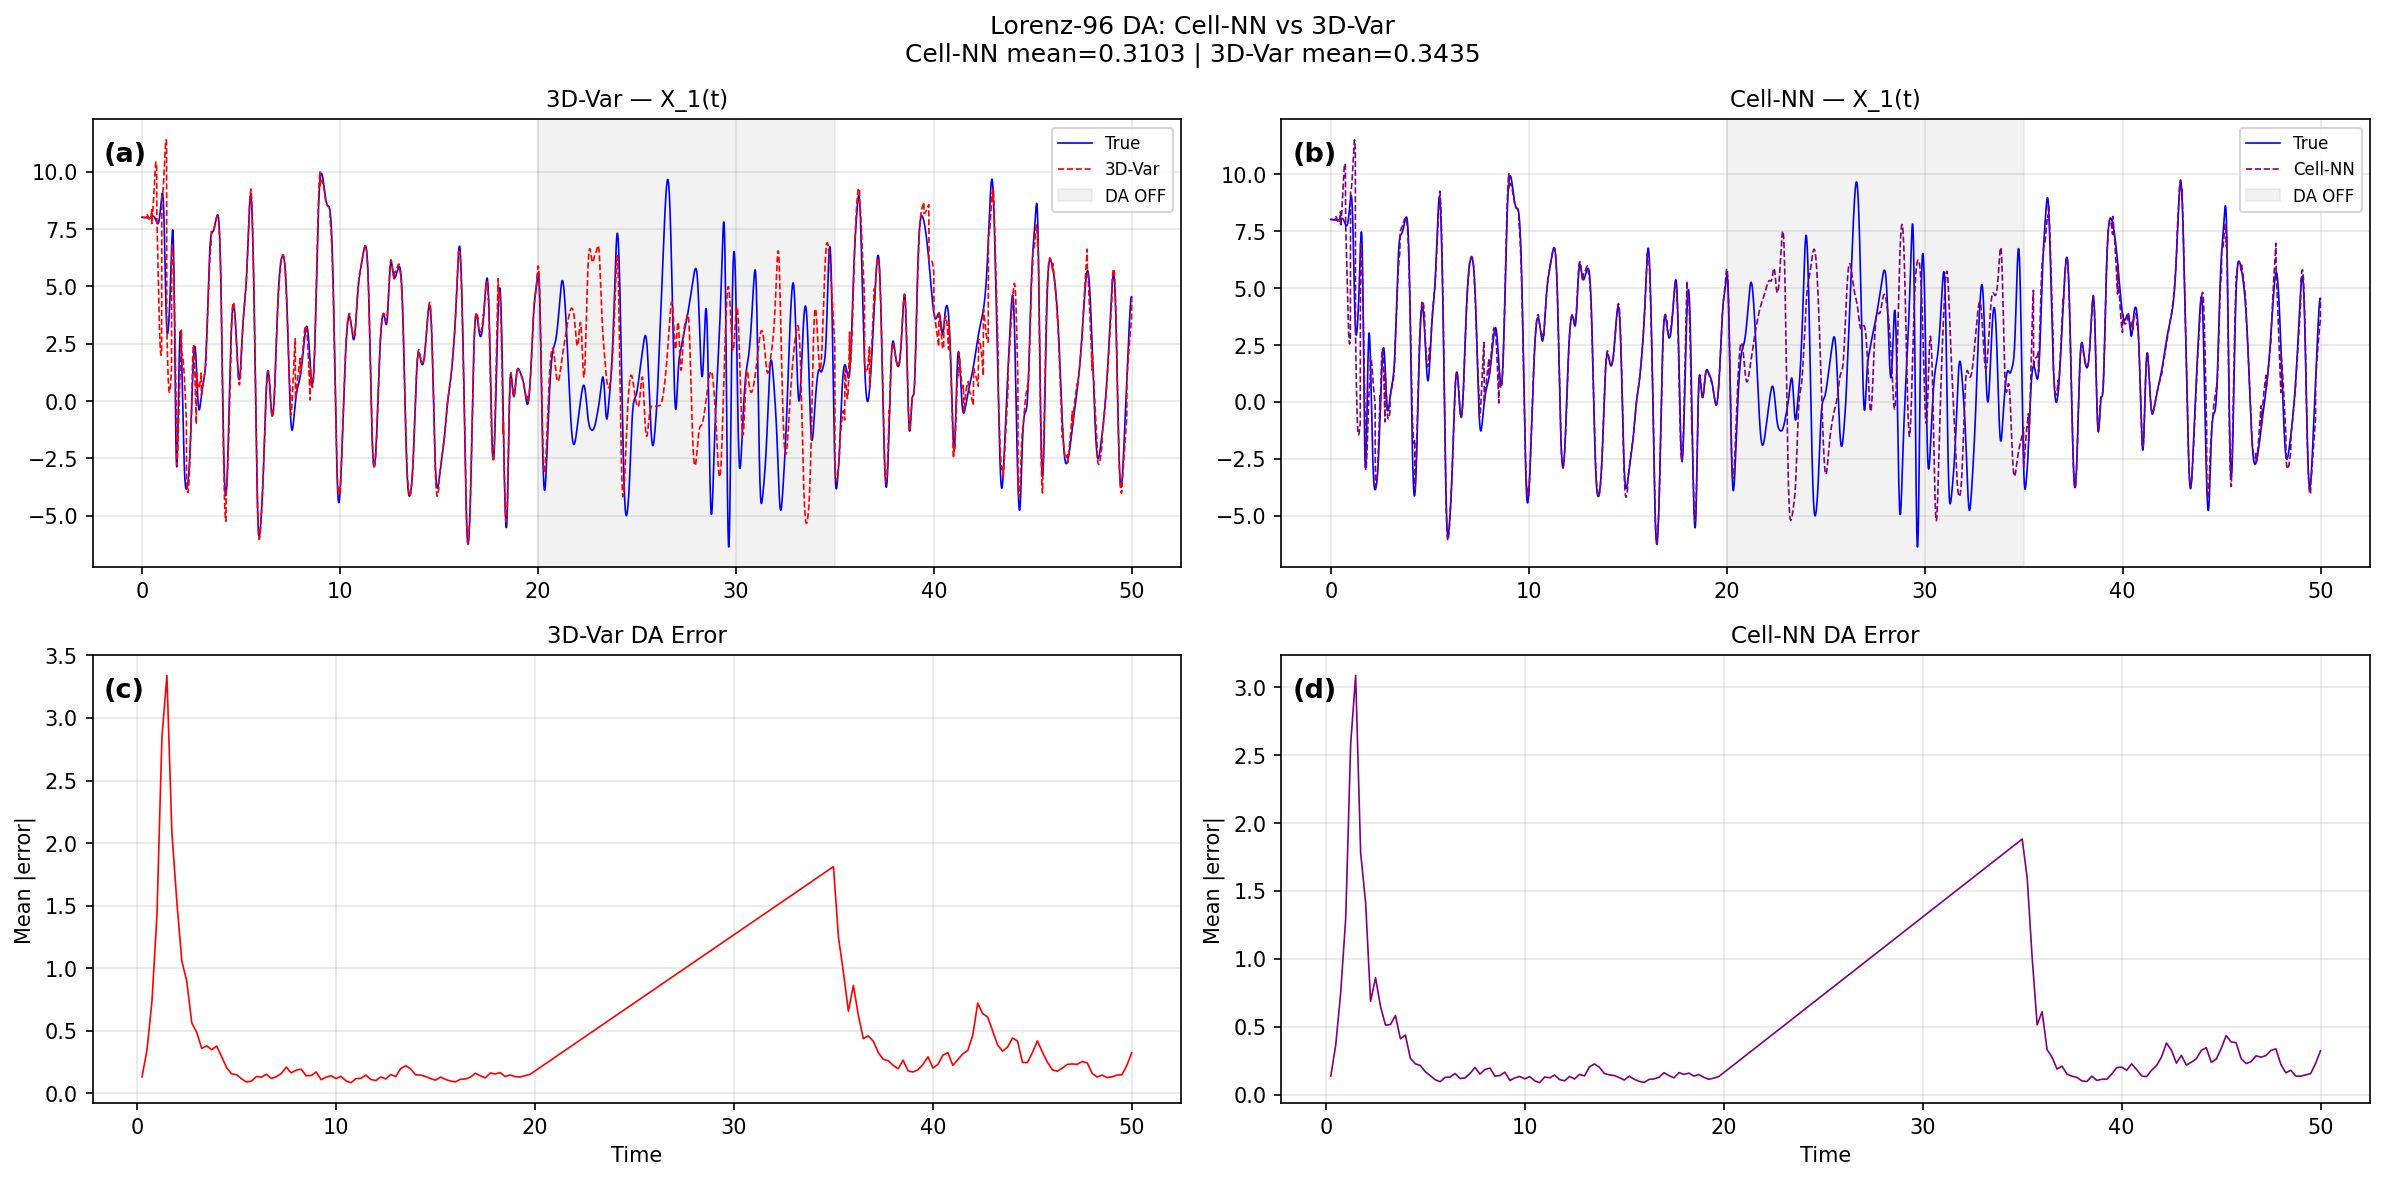
\includegraphics[width=\columnwidth]{Figures/lorenz96_da_comparison.png}
\caption{Lorenz-96 data assimilation comparison: (a) 3D-Var and (b)
Cell-NN reconstructions of $X_1(t)$ against the true trajectory, with
(c) and (d) showing the corresponding DA error over time. Grey shading
marks the DA-off interval ($t=20$--$35$).}
\label{fig:lorenz96_da}
\end{figure}

Figure~\ref{fig:lorenz96_da} shows only $X_1$. Figure~\ref{fig:lorenz96_spatial}
shows all 40 variables at once, for the same realization, as a
function of variable index $k$ and time $t$: (a) true state, (b)
Cell-NN reconstruction, (c) absolute error. The persistent vertical
banding in (a)-(b) reflects each variable's own bias under fixed
forcing $F=8.0$, a structural feature, not an artifact. Panel (c)
shows the DA-off band clearly: mean absolute error is 8.73 times
higher during DA-off (3.77) than DA-on (0.43), confirming the drift
seen in Figure~\ref{fig:lorenz96_da} affects every variable, not only
$X_1$.

\begin{figure*}[t]
\centering
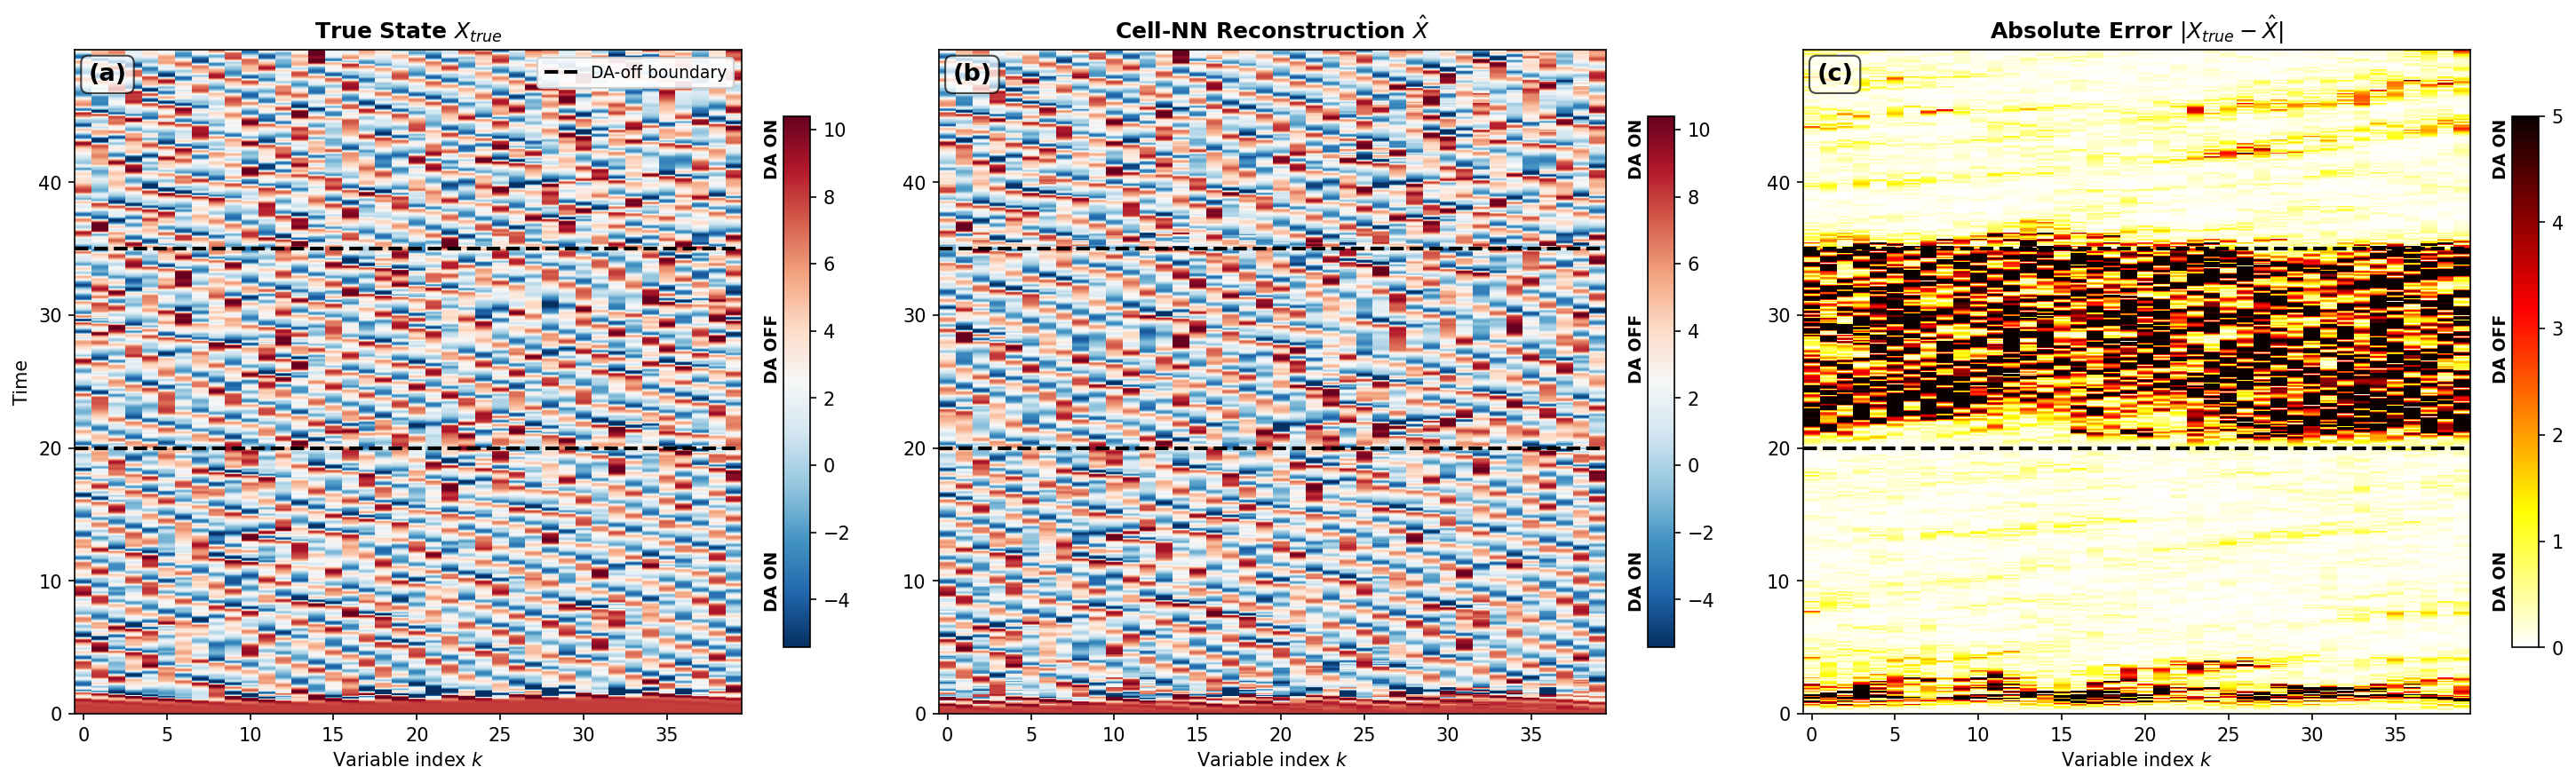
\includegraphics[width=\textwidth]{Figures/lorenz96_spatial_da_onoff.png}
\caption{Full-state Lorenz-96 reconstruction, shown as a function of
variable index $k$ and time $t$, for the same realization as
Figure~\ref{fig:lorenz96_da}. (a) True state. (b) Cell-NN
reconstruction. (c) Absolute error. Dashed lines mark the DA-off
interval ($t=20$--$35$); labels along the right edge of each panel
mark the DA-on and DA-off regions. Mean absolute error is 8.73 times
higher during DA-off (3.77) than during DA-on (0.43).}
\label{fig:lorenz96_spatial}
\end{figure*}

\begin{table}[t]
\centering
\small
\caption{Lorenz-63 reproduction results, no observation-noise or
DA-on/off metrics apply at this scale (Section~\ref{sec:lorenz63}).}
\label{tab:lorenz63_results}
\begin{tabular}{lcc}
\toprule
Method & Error & Training \\
\midrule
3D-Var   & 0.360 & No \\
Cell-NN  & 0.373 & No \\
\bottomrule
\end{tabular}
\end{table}

\begin{table*}[t]
\centering
\caption{Lorenz-96 data assimilation results. R-score and ODE-score
are reported under 5\% observation noise, DA-on periods. EnKF rows
report the same metric under continuous versus irregular observation
availability. Error is not defined for EnKF and 4DVarNet in this
table, since it uses the same per-timestep convention as the 3D-Var
and Cell-NN rows, and is reported here only where directly
comparable.}
\label{tab:lorenz_results}
\begin{tabular}{lcccc}
\toprule
Method & Error & R-score & ODE-score & Training \\
\midrule
3D-Var          & 0.344 & 1.411 & -- & No \\
EnKF (continuous) & --  & 0.005 & -- & No \\
EnKF (irregular) & -- & 23.965 & -- & No \\
Cell-NN (continuous) & 0.310 & 1.245 & $1.79{\times}10^{-13}$ & No \\
Cell-NN (irregular) & -- & 1.245 & -- & No \\
4DVarNet & -- & 0.594 & -- & Yes \\
\bottomrule
\end{tabular}
\end{table*}

\subsection{Robustness under irregular observations}
\label{sec:robustness}

Figure~\ref{fig:enkf_robustness} and the middle rows of
Table~\ref{tab:lorenz_results} summarize the Lorenz-96 experiments
under irregular observations. The tested EnKF formulation is nearly
unaffected by irregular scheduling when localized and tuned for a
continuous network, R-score 0.005, but degrades sharply once
observations become irregular, R-score 23.965, a near 5000-fold
increase. Cell-NN's R-score is unchanged, 1.245 in both regimes.

To check this does not depend on the specific EnKF configuration, we
ran a sensitivity study across ensemble size ($N_\text{ens} \in
\{20, 50, 100, 200\}$), inflation ($\alpha \in \{1.00, 1.02, 1.05,
1.10, 1.20\}$), and localization radius ($r_\text{loc} \in \{4, 6,
8, 10, 14\}$), reporting R-score under both schedules for each
configuration (Table~\ref{tab:enkf_sensitivity}). Every configuration
stable under continuous observations degrades sharply under
irregular ones, from 820-fold worse to complete numerical overflow.

\begin{figure}[ht]
\centering
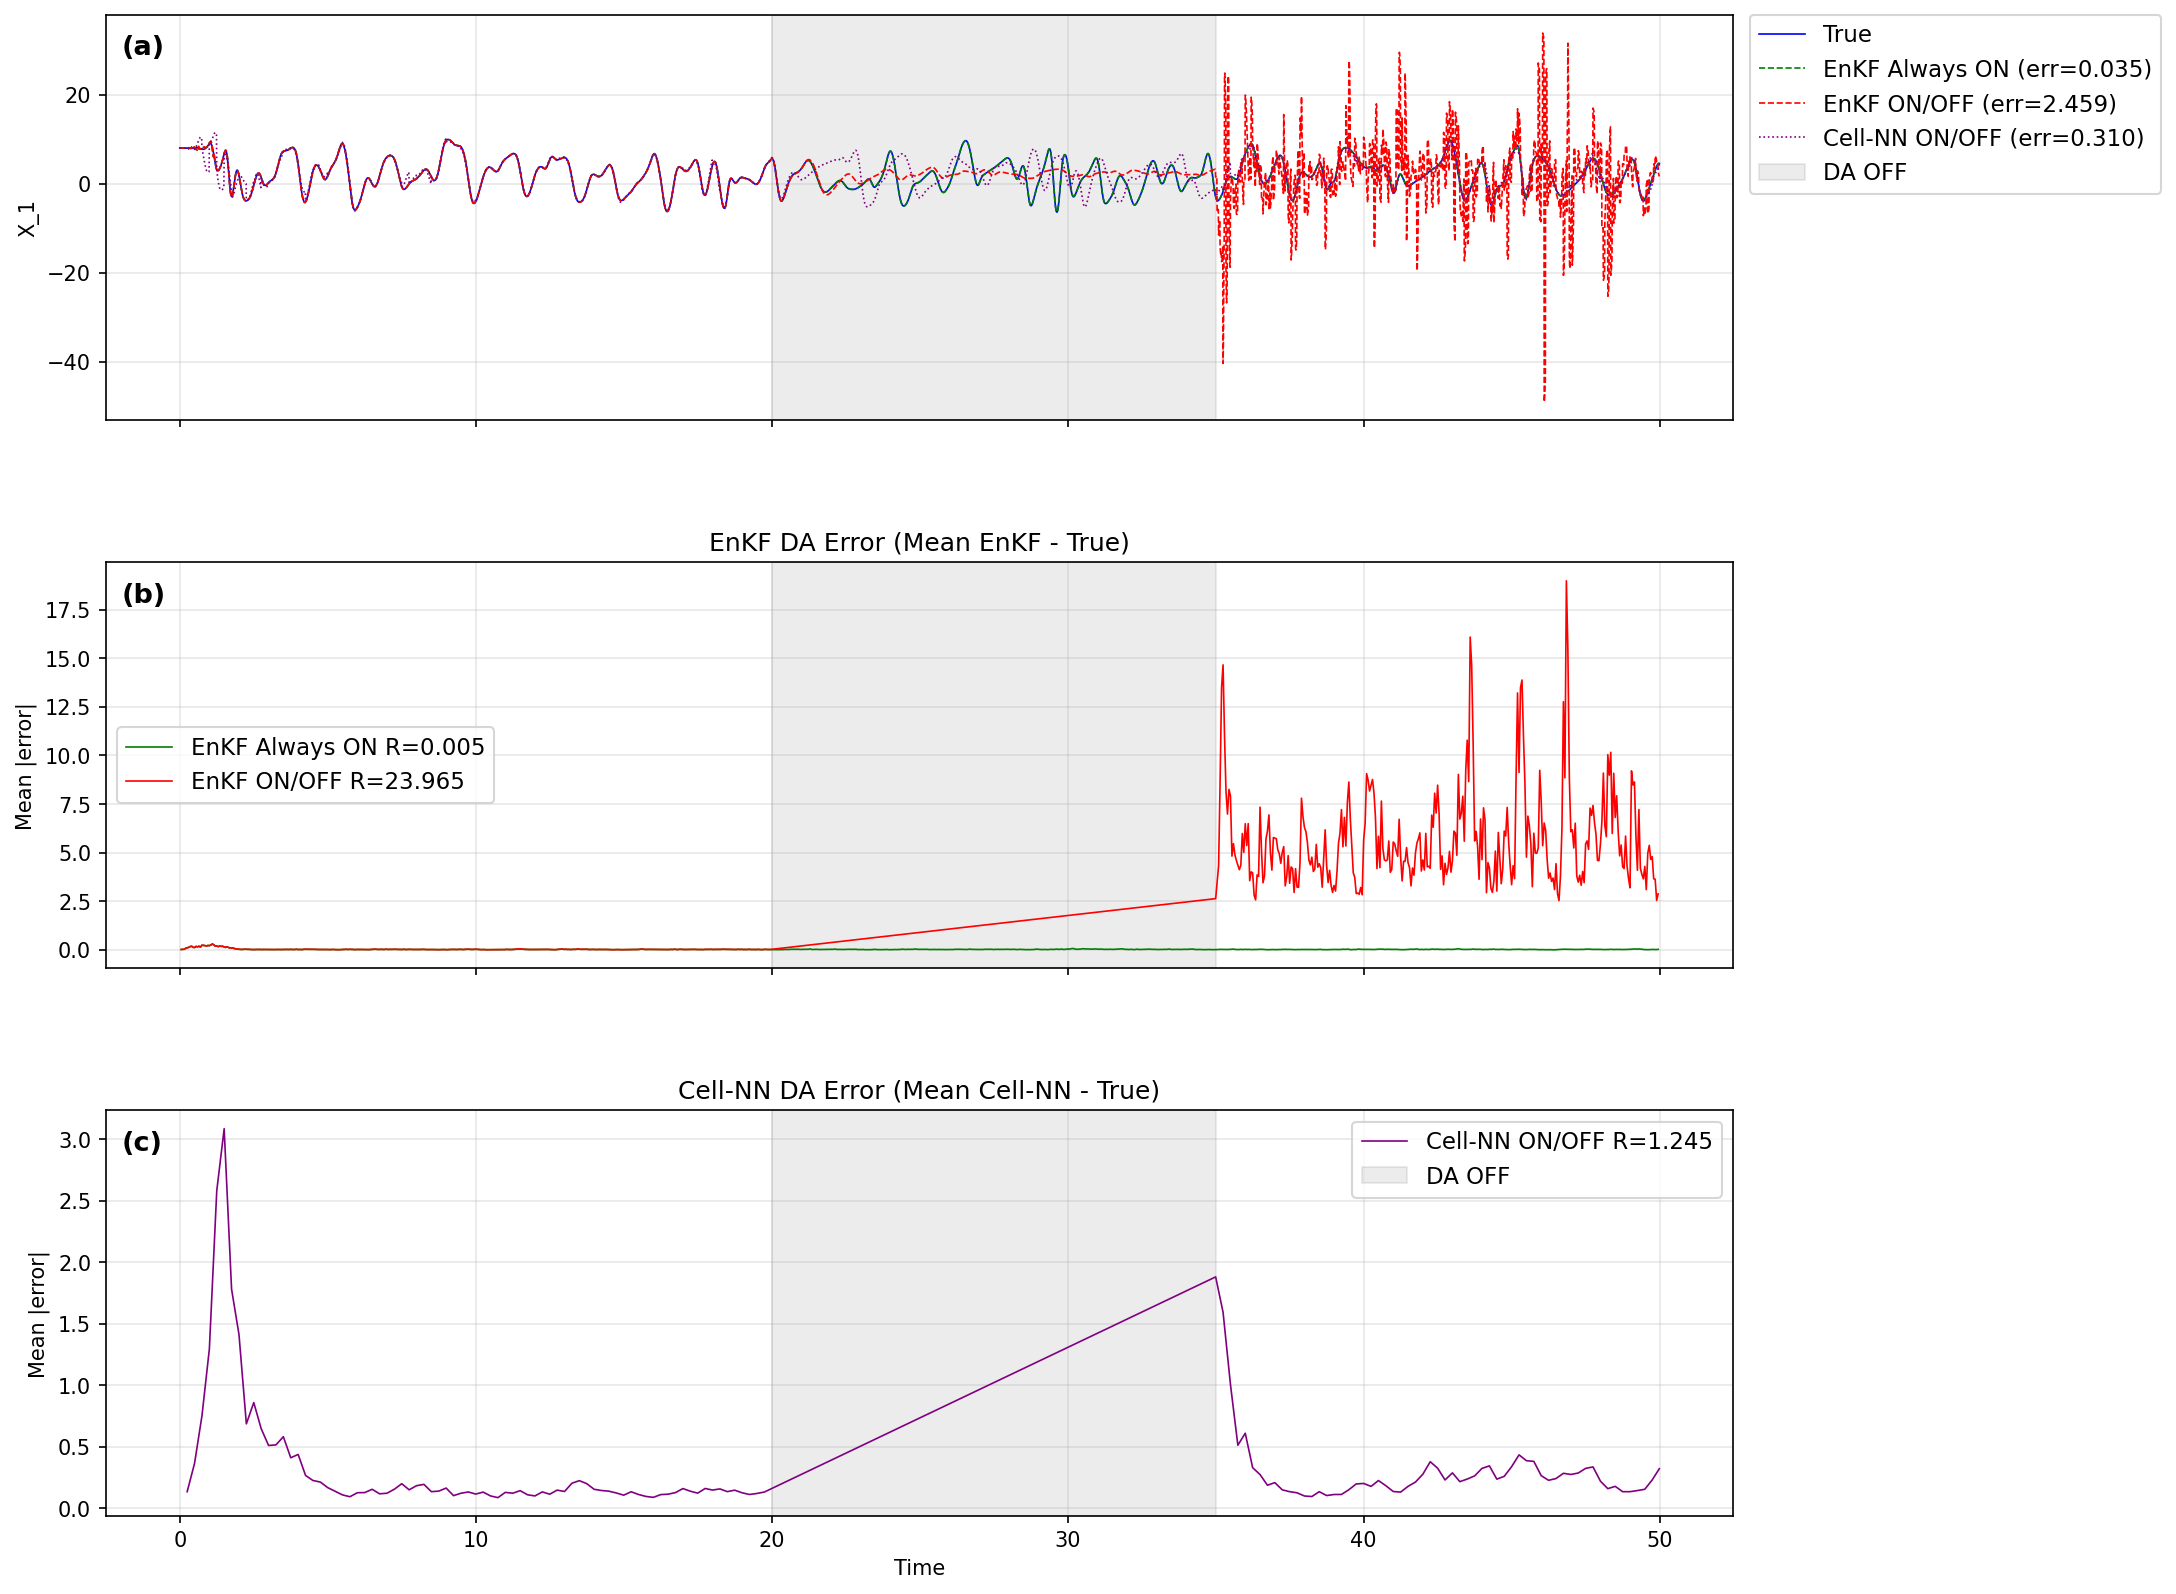
\includegraphics[width=\columnwidth]{Figures/enkf_vs_cellnn_robustness.png}
\caption{EnKF and Cell-NN R-score under continuous versus irregular
observation availability. (a) $X_1(t)$ trajectories for EnKF (always
on and ON/OFF) and Cell-NN (ON/OFF) against the true state. (b) EnKF
DA error (mean absolute deviation from truth) under both schedules.
(c) Cell-NN DA error under the ON/OFF schedule. EnKF shows severe
performance degradation under irregular observations in every tested
configuration; Cell-NN stays stable across both schedules.}
\label{fig:enkf_robustness}
\end{figure}

Ensemble error and spread diagnostics under both schedules are
provided in Supplementary Figure~\ref{fig:enkf_spread}.

\begin{table*}[t]
\centering
\caption{EnKF sensitivity study: R-score under continuous and irregular
observation schedules across parameter configurations. ``$>$100'' denotes
numerical overflow (severe error growth). Configurations already unstable under continuous observations are outside
the valid operating range for this system and do not constitute counter-examples.}
\label{tab:enkf_sensitivity}
\begin{tabular}{lcccc}
\toprule
Parameter & Value & Cont.\ R-score & Interm.\ R-score & Verdict \\
\midrule
\multicolumn{5}{l}{\textit{Varying $N_\text{ens}$ (inflation=1.05, loc.\ radius=8)}} \\
$N_\text{ens}$ & 20  & $>$100 & $>$100 & Outside valid range \\
$N_\text{ens}$ & 50$^\ast$ & 0.005 & 23.965 & Diverges (4699$\times$) \\
$N_\text{ens}$ & 100 & 0.004 & $>$100 & Severe degradation \\
$N_\text{ens}$ & 200 & 0.004 & 3.197   & Diverges (820$\times$) \\
\midrule
\multicolumn{5}{l}{\textit{Varying inflation (N\textsubscript{ens}=50, loc.\ radius=8)}} \\
inflation & 1.00 & 0.003 & $>$100 & Severe degradation \\
inflation & 1.02 & 0.004 & $>$100 & Severe degradation \\
inflation & 1.05$^\ast$ & 0.005 & 23.965 & Diverges (4699$\times$) \\
inflation & 1.10 & $>$100 & $>$100 & Outside valid range \\
\midrule
\multicolumn{5}{l}{\textit{Varying loc.\ radius (N\textsubscript{ens}=50, inflation=1.05)}} \\
loc.\ radius & 8$^\ast$ & 0.005 & 23.965  & Diverges (4673$\times$) \\
loc.\ radius & 10      & 0.004 & 30.733  & Diverges (7674$\times$) \\
loc.\ radius & 14      & 0.003 & $>$100 & Severe degradation \\
\bottomrule
\multicolumn{5}{l}{$^\ast$ = baseline configuration used in the main comparison.}
\end{tabular}
\end{table*}

\textbf{A stronger, adaptively-inflated EnKF variant.} A natural
objection is that this degradation might be an artifact of a fixed,
hand-swept multiplicative inflation constant, rather than a genuine
property of the EnKF family. To test this, we additionally
implemented relaxation-to-prior-spread (RTPS) adaptive inflation
\citep{whitaker2012rtps}, which relaxes posterior ensemble spread
back toward prior spread each cycle, per state variable, rather than
applying one fixed multiplier throughout. Under continuous
observations, RTPS is stable and matches or marginally improves on
fixed inflation: R-score 0.0033--0.0058 across three tested
relaxation parameters ($\alpha \in \{0.1,0.2,0.3\}$), versus 0.005
for fixed inflation.

Under irregular observations, however, RTPS's post-gap behaviour
could not be reduced to a single interpretable R-score. During the
DA-off gap, the ensemble free-runs and its spread decorrelates
chaotically, the same mechanism already documented in
Figure~\ref{fig:lorenz96_spatial}. When RTPS resumes at $t=35$, it
relaxes the new analysis spread back toward this chaos-inflated
prior, treating the gap's own overdispersion as a legitimate
inflation target; this drove the ensemble toward numerical
instability at a rate requiring a hard safety bound to trigger on
99.3\% of post-gap forecast steps, a rate at which the reported
number reflects the safeguard's own arithmetic more than genuine
filter dynamics. We report this honestly rather than presenting an
uninterpretable ratio: a defensible comparison would need gap-aware
inflation logic, outside this study's scope
(Section~\ref{sec:limitations}). Taken together with the fixed-inflation
result, this strengthens rather than weakens the case that the
weakness under irregular observations, seen here in both tested EnKF
formulations, is not simply an artifact of one inflation choice.

\subsection{Cell-NN robustness across gap lengths}

The intermittency experiment above used one schedule (DA-on
0--2000, off 2000--3500, on 3500--5000). To test whether Cell-NN's
stability is schedule-specific, we repeated the 3D-Var versus
Cell-NN comparison across five gap lengths, 0 to 40 DA cycles, 0 to
10 Lorenz time units, averaged over the same five seeds
(Table~\ref{tab:gap_length}).

Cell-NN stays bounded, maximum R-score 1.71, at every tested gap
length, with a positive advantage over 3D-Var in 4 of 5 lengths and
a minor reversal at a 5-cycle gap ($-1.3\%$). Both methods degrade
as gap length increases, but neither shows EnKF's severe degradation
under the block schedule (Section~\ref{sec:robustness}).

\begin{table*}[t]
\centering
\caption{Gap-length robustness: mean R-score across 5 seeds for
3D-Var and Cell-NN under observation gaps of varying duration
(LTU = Lorenz time units; da\_interval=25, $\alpha_A=1.0$).
Cell-NN remains bounded at all gap lengths; positive improvement
in 4 of 5 tested gap durations.}
\label{tab:gap_length}
\begin{tabular}{lrrrr}
\toprule
Gap length & Gap (LTU) & 3D-Var R-score & Cell-NN R-score & Cell-NN improvement \\
\midrule
0 cycles (continuous)   & 0.0  & 1.005 & 0.882 & $+12.2\%$ \\
2 cycles (50 steps)     & 0.5  & 1.039 & 0.909 & $+12.5\%$ \\
5 cycles (125 steps)    & 1.25 & 1.311 & 1.328 & $-1.3\%$  \\
10 cycles (250 steps)   & 2.5  & 1.199 & 1.180 & $+1.6\%$  \\
20 cycles (500 steps)   & 5.0  & 1.250 & 1.129 & $+9.6\%$  \\
40 cycles (1000 steps)  & 10.0 & 1.726 & 1.521 & $+11.8\%$ \\
\bottomrule
\end{tabular}
\end{table*}

\subsection{Comparison with 4DVarNet}

4DVarNet \citep{fablet2021} achieves the lowest R-score among all
methods tested, 0.594, but only after supervised training with
ground-truth trajectories. Among methods needing no supervised
training, Cell-NN achieves the lowest R-score
(Table~\ref{tab:lorenz_results}). Our implementation follows the
published architecture: a convolutional solver trained on 200-step
patches, 20 epochs, batch size 16, Adam, learning rate $10^{-3}$,
R-score computed identically to Cell-NN on DA-on periods only. We
report this comparison to show where Cell-NN sits relative to the
trained end of the spectrum, not as a like-for-like contest given
the training asymmetry.

Table~\ref{tab:cost} summarizes computational requirements. Cell-NN
and 3D-Var have comparable wall-clock times, 4.1 versus 5.2 seconds
for K=40, N=5000, single CPU thread, and near-identical memory
footprints, around 2 MB. EnKF with N=50 members needs about
39$\times$ more compute than Cell-NN here. 4DVarNet needs 20 training
epochs, around 600 seconds, a one-time cost; inference afterward is
comparable to Cell-NN. Complexity follows directly from each method's
structure: Cell-NN touches at most $K$ variables per cycle with a
small, bounded iteration count; 3D-Var solves a linear system
involving the $K\times K$ background-error covariance; EnKF's cost
scales with ensemble size $N_\text{ens}$ plus the per-member forecast
cost.

\begin{table*}[t]
\centering
\caption{Computational cost comparison for Lorenz-96 (K=40, N=5000
steps, da\_interval=25). Wall-clock time averaged over 3 runs on
Apple M-series CPU, single thread. Timings are implementation- and
hardware-dependent; the relative ordering is more informative than
the absolute values. Complexity is asymptotic in state dimension $K$
(and ensemble size $N_\text{ens}$ or dataset size $|\mathcal{D}|$
where relevant), independent of hardware. Training cost for 4DVarNet
is one-time; inference after training is comparable to Cell-NN.}
\label{tab:cost}
\small
\begin{tabular}{@{}l p{2.3cm} r p{3.3cm} l p{2.4cm}@{}}
\toprule
Method & Wall time (s) & Peak RAM (MB) & Complexity & Training & Free params \\
\midrule
3D-Var       & 5.15 & 2.2 & $O(K^2)$ & No  & $\sim K^2$ \\
Cell-NN      & 4.05 & 2.1 & $O(K)$ & No  & 1 ($\alpha_A$) \\
EnKF (N=50)  & $\sim$158$^\dagger$ & 4.8 & $O(N_\text{ens}K)$ + forecast & No  & 3 ($N$, inflation,
loc.) \\
4DVarNet     & $\sim$600s (20 epochs) + $\sim$4s (infer) & --- & infer $O(K)$; train $O(\text{epochs}\!\times\!|\mathcal{D}|)$ & Yes & $\sim$10{,}000 \\
\bottomrule
\multicolumn{6}{l}{$^\dagger$ Approximate; ensemble propagation via
numerical integrator. Optimized}\\
\multicolumn{6}{l}{\phantom{$^\dagger$} EnKF implementations will vary.}
\end{tabular}
\end{table*}

\subsection{Computational scaling with state dimension}
\label{sec:scaling}

Table~\ref{tab:cost} reports cost at one fixed dimension, K=40. To
see how each method actually scales, we timed 3D-Var, Cell-NN, and
EnKF at K$\in\{10,20,40,80,160\}$, N=1000 steps, 1 repeat per point,
a shorter, separate run from Table~\ref{tab:cost}'s K=40-only,
N=5000, 3-repeat timings, built specifically to show the scaling
trend, not to reproduce Table~\ref{tab:cost}'s absolute numbers.

Figure~\ref{fig:scaling} shows the result. EnKF is the clear outlier,
growing from 2.4s at K=10 to 10.5s at K=160, while 3D-Var and Cell-NN
both stay inexpensive and close together across the full range. One
honest caveat: the growth is flatter than the leading-order
complexity terms in Table~\ref{tab:cost} would suggest at these
dimensions, roughly 1.6$\times$ for 3D-Var and 1.3$\times$ for
Cell-NN across a 16-fold increase in K, rather than the
$O(K^2)$/$O(K)$ scaling those terms describe. This indicates that at
K$\leq$160, wall-clock time is dominated by fixed per-cycle overhead,
not by the leading-order term; the complexity classes in
Table~\ref{tab:cost} remain correct statements about the algorithms,
but only become the dominant cost at larger K than tested here. EnKF
consistently dominates cost at every tested dimension, consistent
with its ensemble-propagation overhead.

\begin{figure}[ht]
\centering
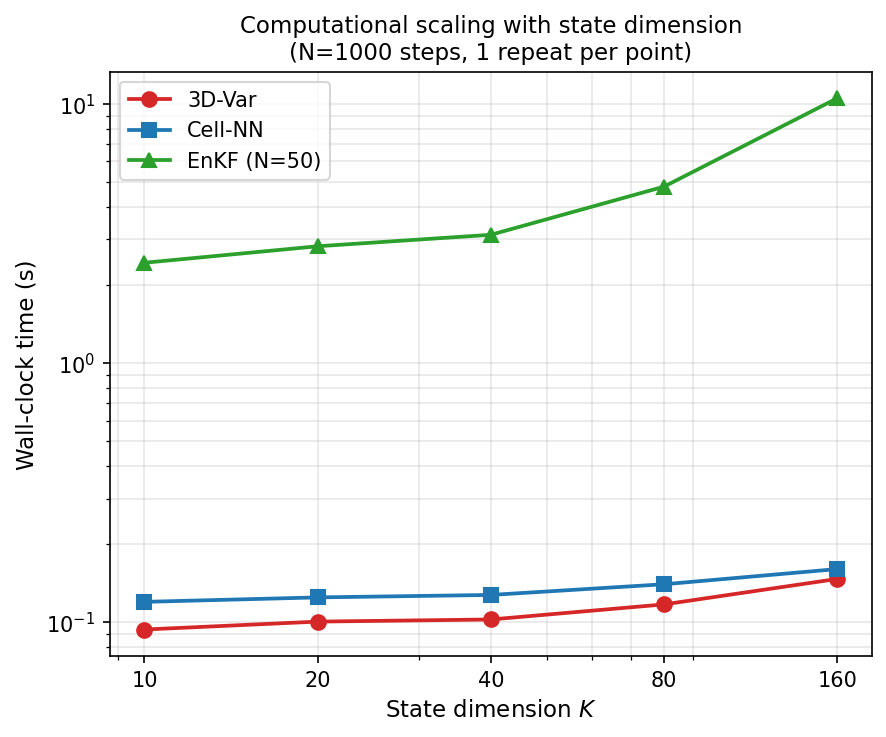
\includegraphics[width=\columnwidth]{Figures/computational_scaling.png}
\caption{Wall-clock time versus state dimension $K$, log-log scale,
for 3D-Var, Cell-NN, and EnKF (N=50 members). N=1000 steps, 1 repeat
per point. EnKF's cost grows fastest and dominates at every tested
$K$; 3D-Var and Cell-NN stay close together and inexpensive
throughout. Growth is flatter than the $O(K^2)$/$O(K)$ complexity
classes in Table~\ref{tab:cost} would suggest at these dimensions,
indicating fixed per-cycle overhead dominates wall-clock cost in this
range, not yet the leading-order asymptotic term.}
\label{fig:scaling}
\end{figure}

\textbf{Extrapolating beyond the tested range.} The tested dimensions,
K$\leq$160, are still small enough that fixed per-cycle overhead
dominates over each method's leading-order term. What would change at
K=1000, a scale closer to a limited-area regional model? Cell-NN
touches each cell once per cycle with a small, bounded number of
relaxation iterations, so its cost should remain close to linear in
K, and its memory footprint, one state vector per cell, stays modest
even at K=1000. 3D-Var's covariance solve, by contrast, involves a
$K\times K$ matrix; at K=1000 this is a $10^6$-element matrix, and
the $O(K^2)$ solve cost this study's Table~\ref{tab:cost} already
states should begin to dominate wall-clock time well before that
scale, rather than being masked by fixed overhead as it is at
K$\leq$160. EnKF's forecast cost scales with $N_\text{ens}$ members
propagated independently, and its analysis step additionally involves
inverting an $n_\text{obs}\times n_\text{obs}$ matrix; at K=1000 with
proportionally more observations, this matrix inversion is likely to
become the dominant cost, compounding the ensemble-propagation
overhead already visible at K$\leq$160 in
Figure~\ref{fig:scaling}. We report this as reasoning from the
complexity classes already established in Table~\ref{tab:cost},
consistent with the empirical trend in Figure~\ref{fig:scaling}, not
as a new empirical claim at K=1000; Section~\ref{sec:future}
identifies a larger benchmark spanning this range as a concrete next
step.

\subsection{Satellite Chl-a reconstruction}
\label{sec:chlresults}

We turn now to the second experimental test: direct satellite
retrieval, the regime where neither condition for cycle-level
assimilation is expected to hold. This is not included as an
application of the Lorenz-96 result to a real dataset; it was chosen
deliberately because it violates the theoretical conditions
Section~\ref{sec:predictions} predicts are needed for genuine
assimilation, making it a controlled test of the diagnostic's
negative prediction, not a showcase of reconstruction performance.
The remaining subsections test the two-condition diagnostic from
Section~\ref{sec:relaxation}: does direct satellite retrieval satisfy
the two conditions for cycle-level background--observation blending?
In this application, Cell-NN is not the primary reconstruction
mechanism; that role belongs to Laplacian diffusion, as the
attribution ablation in Section~\ref{sec:attribution} shows.

Table~\ref{tab:chl_validation} compares five gap-filling methods on
identical held-out test pixels, bootstrap 95\% CIs over 229
timesteps, $n=10{,}000$, all pairwise differences significant at
$p<0.001$. The reconstruction improves RMSE by 82.4\% over the
persistence background, ahead of OI (35.0\%) and DINEOF (45.3\%),
behind only Monte Carlo (84.2\%). Diffusion hyperparameters,
$\kappa=0.4$, 50 iterations, were chosen on the validation subset
(Section~\ref{sec:pipeline}); unjustified default values, $\kappa=0.3$,
30 iterations, give a 76.3\% improvement, RMSE 0.179, 25.2\% worse in
absolute RMSE.

Table~\ref{tab:chl_validation} reports accuracy alone; it is not the
whole story. Table~\ref{tab:sat_cost} times a single-pass
reconstruction of the full 229-composite record for each method.
Cell-NN is the cheapest by a wide margin, 91$\times$ faster than
Monte Carlo, the method that beats it on RMSE, 7.1$\times$ faster
than DINEOF, and 1.4$\times$ faster than OI. DINEOF and Monte Carlo
are not structured per-timestep the way Cell-NN and OI are: DINEOF
performs one global SVD decomposition covering all composites at
once, and Monte Carlo fits one distribution per pixel from the whole
record, then reuses it across every reconstructed date; the
per-timestep column below is a normalized figure for comparison, not
a literal description of either method's computational pattern. Read
together with Table~\ref{tab:chl_validation}, Monte Carlo's 1.8
percentage-point RMSE advantage over Cell-NN comes at roughly
91$\times$ the computational cost, a trade-off the accuracy numbers
alone do not convey.

\begin{table}[t]
\centering
\small
\caption{Satellite pipeline cost comparison: single-pass wall-clock
time to reconstruct the full 229-composite record, Apple M-series
CPU, single thread. DINEOF and Monte Carlo perform one batch
computation (SVD decomposition; per-pixel distribution fit) rather
than per-timestep updates, so their per-timestep column is a
normalized figure for comparison, not a literal per-cycle cost.}
\label{tab:sat_cost}
\begin{tabular}{lcc}
\toprule
Method & Wall time (s) & Per-timestep (s) \\
\midrule
Cell-NN pipeline & 11.9 & 0.052 \\
OI               & 16.3 & 0.071 \\
DINEOF           & 84.6 & 0.369 \\
Monte Carlo      & 1{,}080.0 & 4.716 \\
\bottomrule
\end{tabular}
\end{table}

Figure~\ref{fig:multimethod} shows all five methods side by side, on
four composites spanning the observed cloud-coverage range, labeled
(a)--(d): 14.3\%, 40.2\%, 70.5\%, 89.9\%. The figure has eight rows:
the observation mask, derived from MODIS L3 coverage; filled ground
truth, from L4, never given to any method as input; three
deterministic methods, OI, DINEOF, Cell-NN with diffusion; and three
Monte Carlo rows, ensemble mean and two individual stochastic draws.
Ground truth is placed second, immediately after the mask, so every
reconstruction row below it can be compared directly against it.
Monte Carlo gets three rows because it is stochastic, drawing from a
per-pixel distribution; every other method is deterministic,
producing one fixed output. A filled reference is needed rather than
MODIS's own gappy field because every method's reconstruction is
complete, with a value at every pixel including ones MODIS itself
never observed; a complete reconstruction needs a complete reference
to be judged fairly everywhere.

One pattern deserves explicit comment: OI's behaviour in column (a),
at 14.3\% coverage, shows large, smooth, visibly wrong patches,
unlike its behaviour at higher coverage. This is a known failure mode
of Gaussian-kernel interpolation under very sparse observations, where
the covariance matrix used for the analysis becomes nearly singular;
it is a structural weakness of the method, not an implementation bug,
and part of why OI trails Cell-NN and DINEOF in
Table~\ref{tab:chl_validation}.

\begin{figure*}[t]
\centering
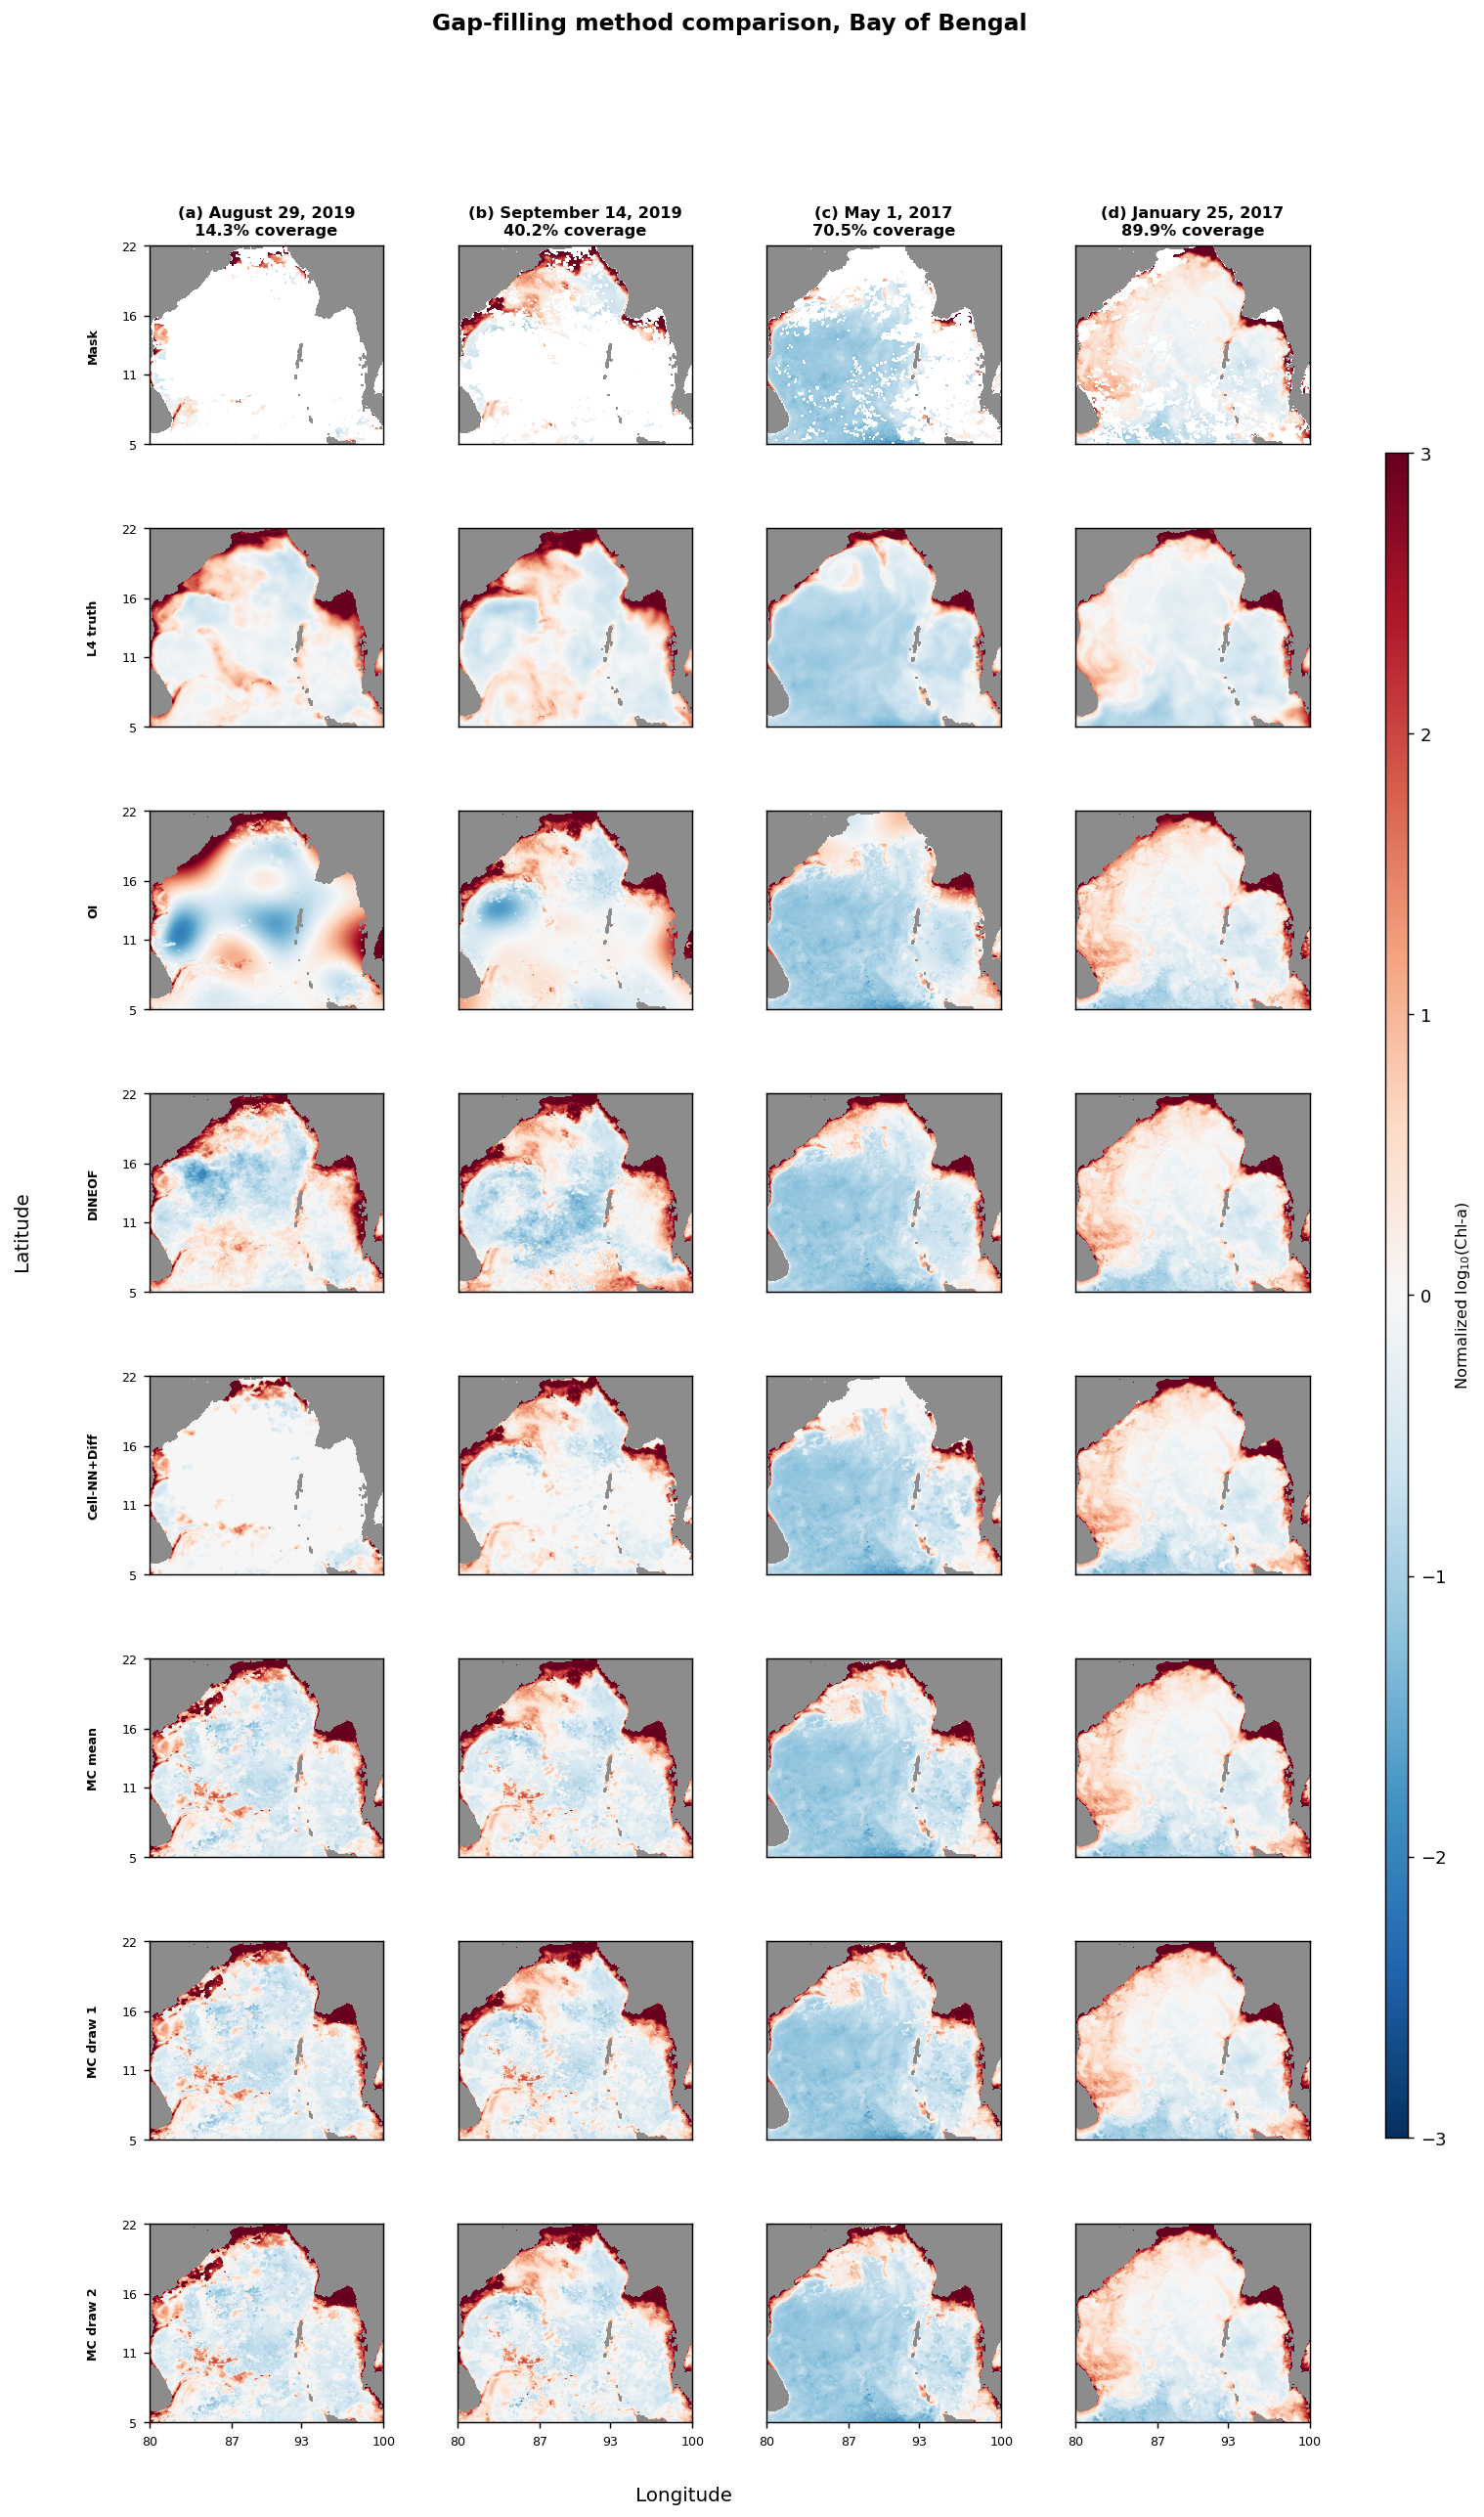
\includegraphics[width=\textwidth,height=0.85\textheight,keepaspectratio]{Figures/multimethod_merged.png}
\caption{Gap-filling method comparison across four composites
spanning the observed range of cloud coverage, labeled (a)--(d):
August 29, 2019 (14.3\% coverage), September 14, 2019 (40.2\%), May
1, 2017 (70.5\%), and January 25, 2017 (89.9\%). Rows, top to
bottom: the observation mask, derived from MODIS L3 coverage; filled
ground truth from the L4 product, never supplied to any method as
input; OI; DINEOF; Cell-NN with diffusion; and the Monte Carlo
ensemble mean and two individual stochastic draws. OI shows large,
unstable patches at 14.3\% coverage (column a), a known
Gaussian-kernel-interpolation failure mode under very sparse
observations, not an implementation error.}
\label{fig:multimethod}
\end{figure*}

Reconstruction error at held-out pixels is not spatially uniform:
binning into coarse regions shows the largest mean errors in the
southeastern domain, near the Andaman Sea, mean absolute error 0.214,
roughly four times the domain-wide mean of 0.054. Temporal cloud
coverage there is comparable to the central Bay of Bengal, where
error is much lower, 0.022, so reduced coverage does not explain the
elevated error. Instead, the southeastern region is a narrow coastal
strip with only 1,833 ocean pixels, 61\% land, compared to 15,288
ocean pixels centrally; this spatial isolation, few nearby ocean
neighbours for diffusion to draw from, is a more likely driver,
consistent with Section~\ref{sec:cloudmask}'s finding that
improvement declines with contiguous gap size, not aggregate coverage
fraction.

\begin{table*}[t]
\centering
\caption{MODIS Chl-a internal gap-filling comparison (random 20\%
held-out pixels; diffusion parameters $\kappa=0.4$, 50 iterations
selected on the validation subset, Section~\ref{sec:pipeline}; all
figures below scored on the disjoint test subset). RMSE and 95\%
bootstrap CIs in normalized (log$_{10}$ + z-score) units. All
pairwise differences $p<0.001$ ($n=10{,}000$ resamples, 229
timesteps).}
\label{tab:chl_validation}
\begin{tabular}{lccc}
\toprule
Method & RMSE [95\% CI] & Improvement [95\% CI] & Historical data \\
\midrule
Background (persistence)   & 0.7548 [0.7296, 0.7803] & -- & No \\
OI ($L=0.20$, Gaussian)   & 0.4909 [0.4776, 0.5055] & 35.0\% [32.9\%, 37.0\%] & No \\
DINEOF ($r=17$ EOFs)       & 0.4125 [0.3965, 0.4289] & 45.3\% [44.0\%, 46.6\%] & No \\
Diffusion pipeline ($\kappa=0.4$, $n=50$) & 0.1330 [0.1292, 0.1369] & 82.4\% [82.1\%, 82.7\%] & No \\
Monte-Carlo (causal, \citealt{modi2022montecarlo}) & 0.1195 [0.1169, 0.1223] & 84.2\% [83.8\%, 84.6\%] & Yes \\
\bottomrule
\end{tabular}
\end{table*}

\subsection{Fixed-region reconstruction test}
\label{sec:rectmask}

Sections~\ref{sec:attribution} and~\ref{sec:noisesweep} both show
numerically that reconstruction skill at unobserved pixels comes
entirely from diffusion. This section provides a direct visual
counterpart, using one controlled spatial test rather than pixels
scattered across the domain.

We select a 60$\times$60 pixel square south of the Indian coast,
11.6--14.1$^{\circ}$N, 80.0--82.5$^{\circ}$E. This region was not the
first tried: an earlier southeastern candidate near the Andaman Sea
failed a stability check, its RMSE got worse, not better, as the
diffusion budget increased, because a real coastline shifts position
slightly between composite dates, and diffusion cannot recreate a
moved sharp boundary. The region used here tests as stable instead:
improvement grows from 23.7\% to 32.5\% as diffusion iterations
increase from the production default to a much larger budget, the
correct, expected signature of a genuinely stable test region.

The square is 6\% land, 94\% ocean; MODIS reports valid observations
at 99\% of its ocean pixels on the target date. We deliberately
withhold every pixel inside from the Cell-NN relaxation step, so it
receives zero observed pixels. Since Cell-NN only updates pixels with
a valid current observation, the entire reconstruction inside the
square comes from diffusion alone, a direct experimental analogue of
Configuration B in Table~\ref{tab:attribution}, applied to one
isolated region rather than scattered pixels.

Ground truth here is L4, not MODIS's own value, since MODIS may lack
a valid retrieval at some pixels inside the square on the target
date. Outside the square, the reconstruction panel is the pipeline's
ordinary, complete output; only the hidden square's pixels differ,
because they start from zero observed pixels rather than a partial
observation.

Figure~\ref{fig:rectmask} shows four panels: (a) the observation
mask, land, the hidden square, and natural cloud gaps shown in the
same excluded colour, since only actively-used input receives a
distinct colour; (b) the L4 ground truth; (c) the full pipeline
reconstruction; (d) the absolute error against L4.

The reconstruction reduces RMSE against L4 from 0.571 to 0.436, a
23.7\% improvement over $n=3{,}351$ scored pixels, at the production
setting; extending to $n=1{,}000$ diffusion iterations increases the
improvement to 32.5\%, confirming genuine stability rather than a
lucky stopping point. The reconstruction is visibly smoother than the
surrounding L4 field inside the square, consistent with diffusion's
low-pass character (Section~\ref{sec:trend}): since the square is
entirely unobserved, nothing in the pipeline can recover fine
texture, only the broad spatial pattern and magnitude. This is the
expected, not defective, consequence of the two-condition
diagnostic: with zero observed pixels inside the square, neither
condition for Cell-NN blending can apply there. The figure is, in
effect, a picture of what Table~\ref{tab:attribution} already
establishes numerically.

To check whether this pattern is an artifact of the one region shown
in Figure~\ref{fig:rectmask}, we additionally tested five further
regions, sampled from a systematic grid (60$\times$60 pixels, 80-pixel
stride, ocean fraction $\geq$70\%) with a fixed random seed, chosen
before any RMSE was computed, and explicitly excluding the region
shown in Figure~\ref{fig:rectmask}. All five show positive
improvement (range 0.8\%--21.5\%, mean 10.6\%, $n=5$), confirming
that diffusion alone recovers meaningful skill in a completely
unobserved region across a range of locations, not only the one
selected for the figure. We report transparently that the region in
Figure~\ref{fig:rectmask} achieves the highest improvement among the
six regions checked here, 23.7\% against the blind sample's mean of
10.6\%, rather than omit this. It was not chosen for that reason: it
was chosen because it verified stability under an extended diffusion
budget, after an initial candidate near the Andaman Sea failed this
check, its RMSE worsened, not improved, with more diffusion
iterations, traced to a real coastline that shifts position between
the composite dates being compared, which diffusion cannot recreate.
The wide range across the blind sample likely reflects the same
spatial-isolation factor discussed in Section~\ref{sec:chlresults}:
regions with fewer nearby ocean neighbours for diffusion to draw
from recover less skill, independent of which specific region is
tested.

\begin{figure*}[t]
\centering
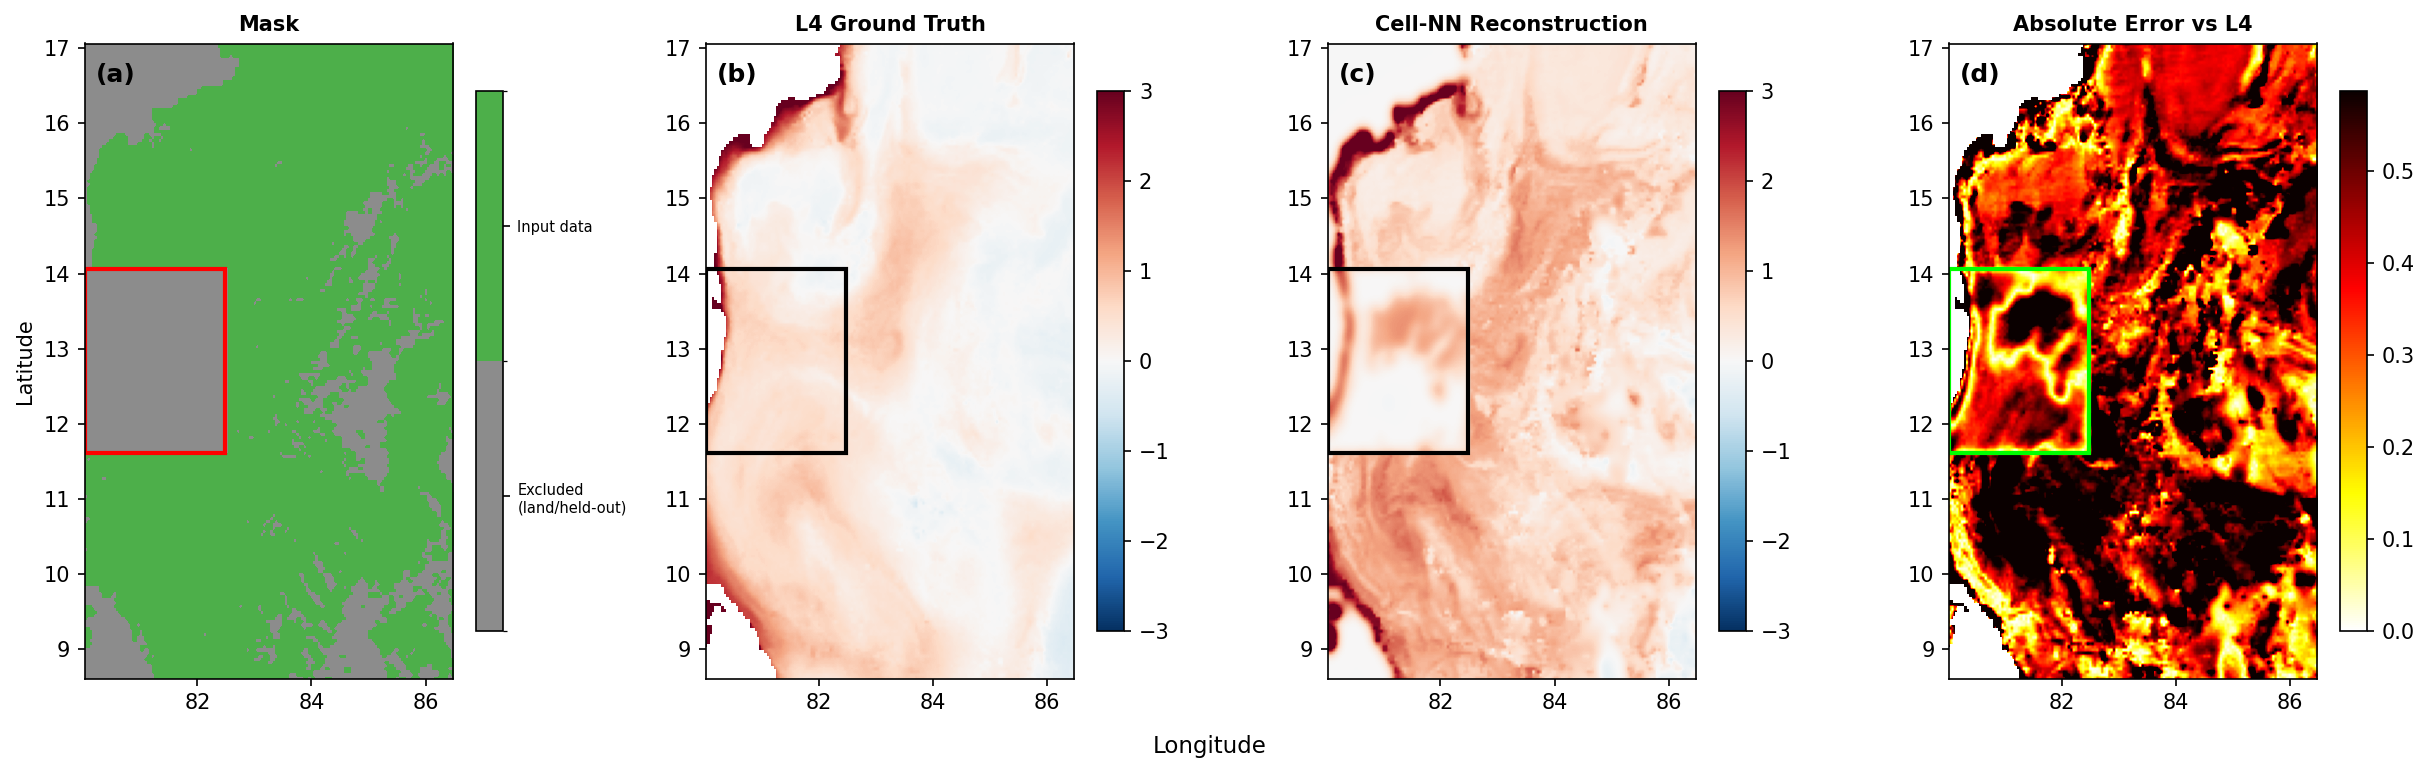
\includegraphics[width=\textwidth]{Figures/rect_mask_final.png}
\caption{Fixed-region reconstruction test. A 60$\times$60 pixel
square (11.6--14.1$^{\circ}$N, 80.0--82.5$^{\circ}$E, south of the
Indian coast) is entirely withheld from the Cell-NN relaxation step,
so its reconstruction comes from diffusion alone. Panels, left to
right: (a) the observation mask, with land, the hidden test square,
and natural cloud gaps shown in the same excluded colour; (b) the L4
ground truth; (c) the full pipeline reconstruction; (d) the absolute
error against L4. RMSE improves from 0.571 (background) to 0.436
(reconstruction), a 23.7\% improvement over $n=3{,}351$ scored
pixels, growing to 32.5\% at $n=1{,}000$ diffusion iterations.}
\label{fig:rectmask}
\end{figure*}

\subsection{External validation against an independent reference}
\label{sec:l4validation}

We validated the reconstruction against L4 (Section~\ref{sec:datasets}),
never supplied to the pipeline as input. For every date, we withhold
the same 20\% random mask used internally, reconstruct the withheld
pixels, and compare against L4 at those pixels and dates, on the raw
$\log_{10}$ scale.

Averaged over 229 composites, the persistence background reaches an
RMSE of 0.229 against L4, while the Cell-NN pipeline reaches 0.101, a
56.0\% improvement. Pooling all 3.63 million held-out comparisons,
reconstructed values correlate with L4 at $R^2=0.92$, slope 1.04,
close to the ideal 1.0; the persistence background alone reaches only
$R^2=0.51$, slope 0.64, showing it systematically compresses true
variation. The pooled RMSE in Figure~\ref{fig:l4_validation} (0.219
background, 0.100 Cell-NN) differs slightly from the composite-mean
values above because $R^2$ and slope pool every pixel-level
comparison while the RMSE above is the mean of per-composite RMSE;
both aggregations show the same pattern.

This differs from the improvement measured against MODIS's own
withheld pixels (82.4\%), which is expected, not contradictory: L4
is itself interpolated, so it carries less small-scale noise than a
raw retrieval, and a smoothing-based reconstruction naturally shows a
smaller relative improvement against an already-smooth reference. The
pipeline still explains most of the variance ($R^2=0.92$) and
recovers magnitude closely (slope 1.04), the more informative
comparison against an external product.

Figure~\ref{fig:l4_validation} shows this as a scatter density plot:
(a) persistence background versus L4, (b) Cell-NN pipeline versus L4,
dashed white line the ideal 1:1 relationship, solid red line the
fitted regression, colour showing point density on a log scale. Panel
(b)'s points sit visibly closer to 1:1 than panel (a)'s.

\begin{figure}[ht]
\centering
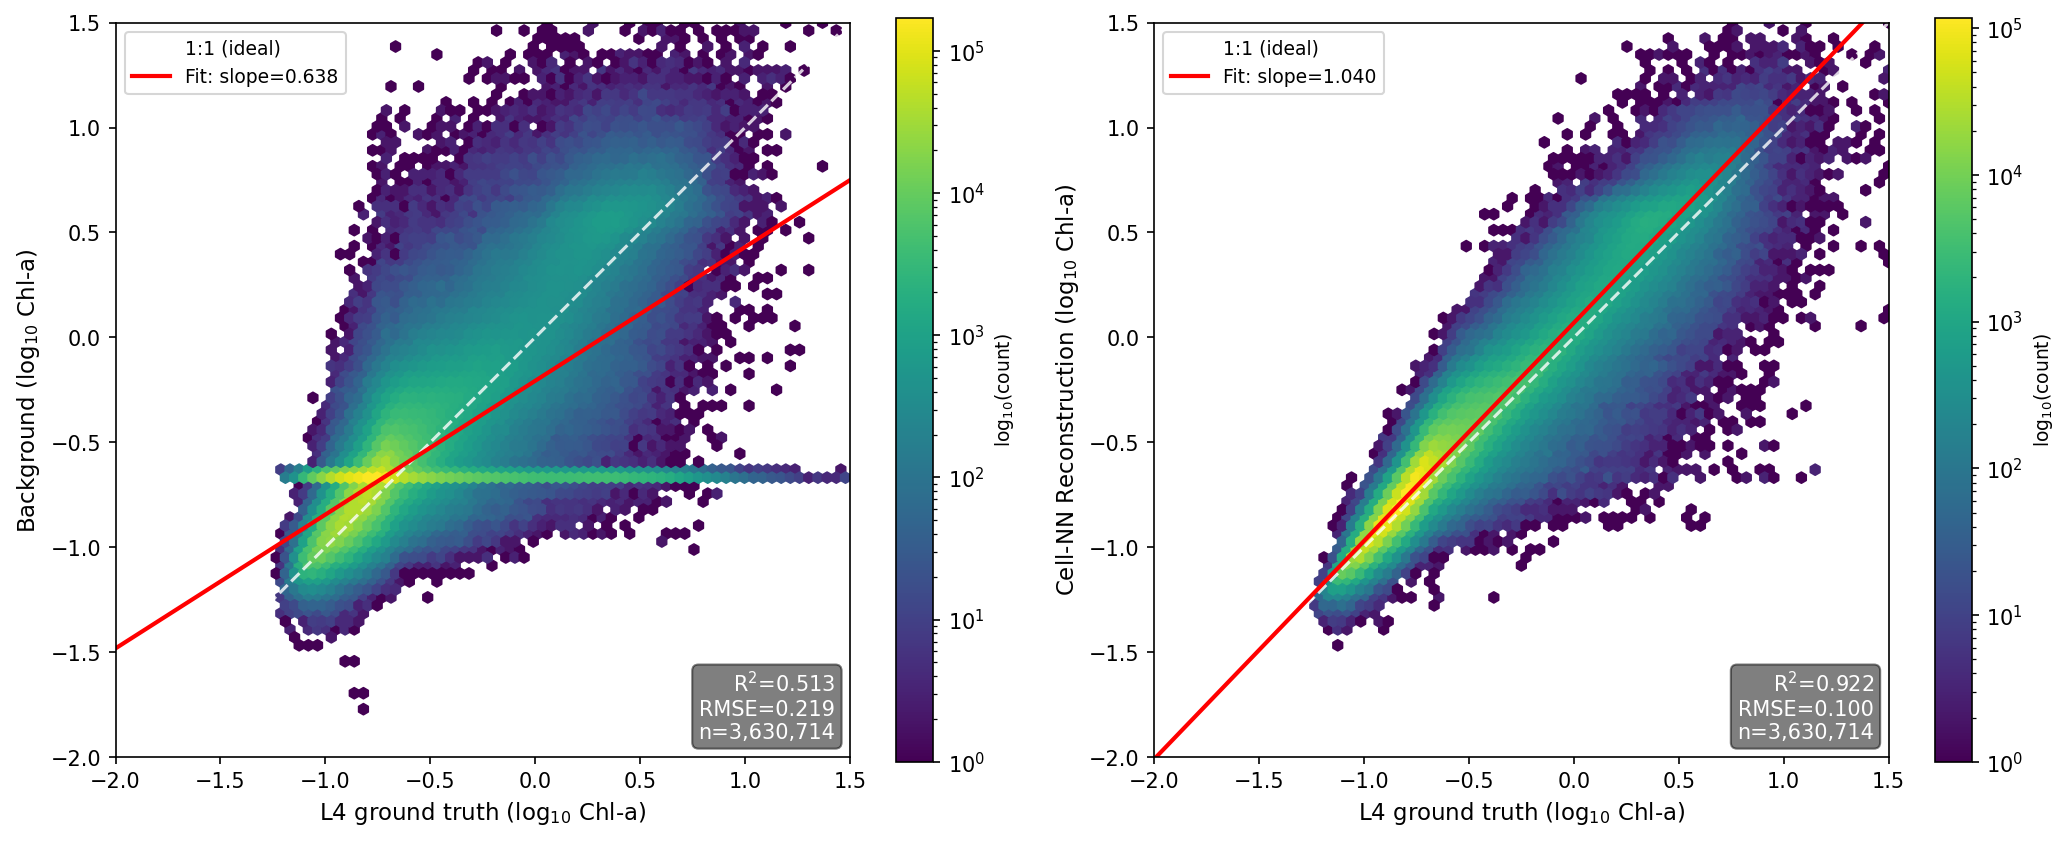
\includegraphics[width=\columnwidth]{Figures/l4_predicted_vs_actual.png}
\caption{Reconstructed values against the independent L4 reference,
pooled across 3.63 million held-out pixels. (a) Persistence
background. (b) Cell-NN pipeline. Dashed white line: ideal 1:1
relationship. Solid red line: fitted regression. Colour shows point
density on a log scale. Panel (b)'s tighter clustering around the
1:1 line shows the pipeline tracks true variation against an
independent reference, not only against the MODIS pixels used to
tune it.}
\label{fig:l4_validation}
\end{figure}

Table~\ref{tab:master_metrics} consolidates the satellite methods'
performance across both validation protocols. $R^2$ and slope
against L4 were computed only for the persistence background and the
Cell-NN pipeline, the two fields directly compared in
Figure~\ref{fig:l4_validation}; OI, DINEOF, and Monte Carlo were not
evaluated against L4 in this study, and we mark this explicitly
rather than omit the columns. EnKF is a Lorenz-96 baseline
(Table~\ref{tab:lorenz_results}), evaluated by a different metric
convention (R-score, ODE-score) on a different system entirely, and
so is not included here.

\begin{table*}[t]
\centering
\caption{Consolidated satellite reconstruction performance. RMSE (vs
MODIS) and improvement are from Table~\ref{tab:chl_validation}, the
internal validation against MODIS's own held-out pixels. RMSE (vs
L4), $R^2$, and slope are from Section~\ref{sec:l4validation}, the
external validation against the independent L4 product; these were
computed only for the persistence background and the Cell-NN
pipeline. EnKF, a Lorenz-96 baseline evaluated by a different metric
convention on a different system, is reported separately in
Table~\ref{tab:lorenz_results}.}
\label{tab:master_metrics}
\begin{tabular}{lccccc}
\toprule
Method & RMSE (vs MODIS) & Improvement & RMSE (vs L4) & $R^2$ (vs L4) & Slope (vs L4) \\
\midrule
Background (persistence) & 0.7548 & -- & 0.229 & 0.51 & 0.64 \\
OI                       & 0.4909 & 35.0\% & not computed & not computed & not computed \\
DINEOF                   & 0.4125 & 45.3\% & not computed & not computed & not computed \\
Cell-NN pipeline         & 0.1330 & 82.4\% & 0.101 & 0.92 & 1.04 \\
Monte Carlo              & 0.1195 & 84.2\% & not computed & not computed & not computed \\
\bottomrule
\end{tabular}
\end{table*}

\subsection{Trend and seasonal-amplitude recovery}
\label{sec:trend}

The reconstruction systematically damps long-term trend amplitude
(Table~\ref{tab:trend}, Figure~\ref{fig:trend}). The true basin-mean
trend, $+0.0494$ yr$^{-1}$, is recovered as $+0.0266$ yr$^{-1}$, a
46\% reduction; the median trend, $+0.0410$ yr$^{-1}$, as $+0.0163$
yr$^{-1}$, a 60\% reduction. Figure~\ref{fig:trend} shows basin-mean
(a) and basin-median (b) time series, true field versus reconstruction
with linear trend fits; the reconstructed slope visibly sits below
the true slope in both panels. An independently reported result for
global Chl-a reconstruction finds the same pattern of underestimated
low-frequency amplitude across four UNet-family model variants
\citep{martinez2020frontiers}.

\begin{table*}[t]
\centering
\caption{Basin-mean Chl-a trend recovery, 2015--2019.}
\label{tab:trend}
\begin{tabular}{lccc}
\toprule
Metric & True & Cell-NN reconstructed & Damping \\
\midrule
Mean trend (yr$^{-1}$)   & $+0.0494$ & $+0.0266$ & $-46\%$ \\
Median trend (yr$^{-1}$) & $+0.0410$ & $+0.0163$ & $-60\%$ \\
\bottomrule
\end{tabular}
\end{table*}

\begin{figure}[ht]
\centering
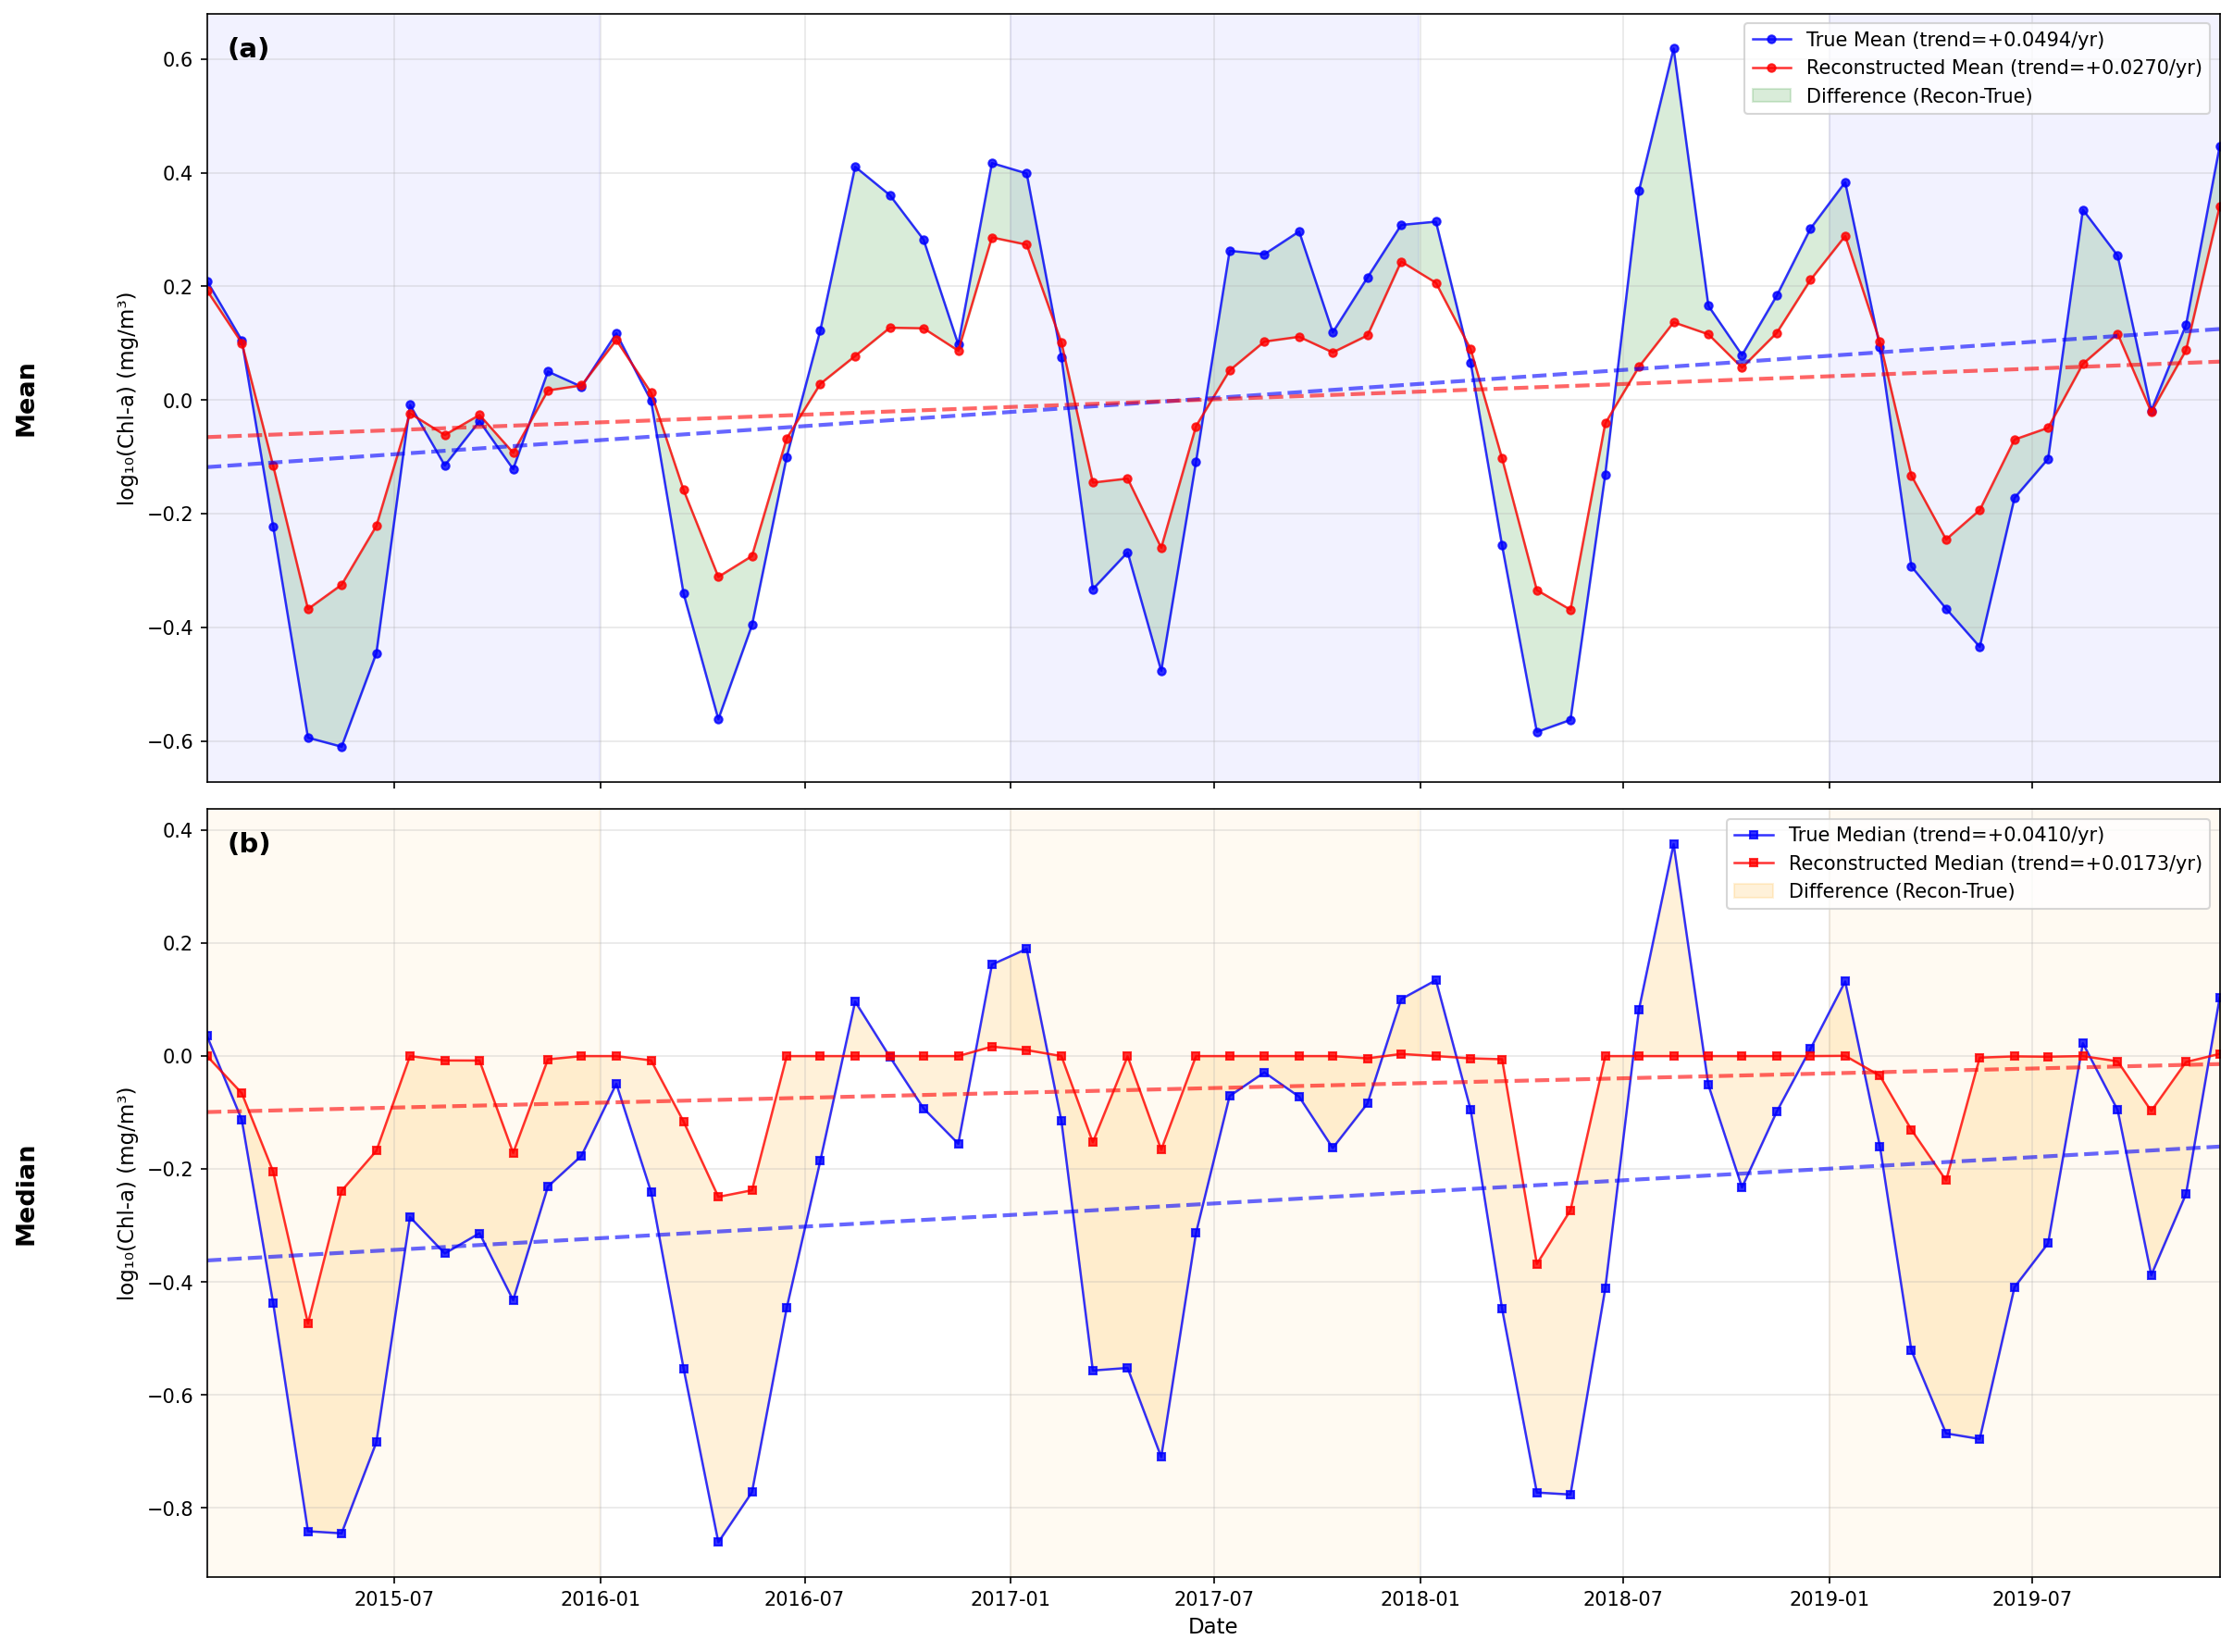
\includegraphics[width=\columnwidth]{Figures/chl_mean_median_comparison.png}
\caption{Basin-mean and basin-median Chl-a time series, true field
versus Cell-NN reconstruction, with linear trend fits. Mean and
median are shown in panels (a) and (b) respectively; each panel shows
the true field, the Cell-NN reconstruction, and their difference over
2015--2019. The reconstructed slope's visible shortfall against the
true slope in both panels is the trend damping
Table~\ref{tab:trend} reports as a number.}
\label{fig:trend}
\end{figure}

\subsection{Seasonal robustness of gap-filling performance}
\label{sec:seasonal}

Supplementary Table~\ref{tab:seasonal} stratifies internal validation
by Bay of Bengal season, test subset, $\kappa=0.4$, $n=50$. SW
monsoon composites have 29.6\% mean valid coverage, less than half
the NE monsoon's 70.6\%, yet the reconstruction achieves comparable
improvement across all three seasons: 82.7\%, 81.7\%, 82.7\%.
Background RMSE is higher during SW monsoon (0.931) than
Pre/Post-monsoon (0.629), reflecting lower background quality when
persistence must bridge a longer or more severe gap.

\subsection{Spatial snapshot, 1 January 2016}

Supplementary Figure~\ref{fig:snapshot} compares the MODIS observed
field (63.4\% valid), the Cell-NN reconstruction (100\% coverage),
and the L4 reference field for one date. The reconstruction is
visibly smoother in the open-ocean interior than the texture in the
MODIS valid pixels, the same low-pass character discussed in
Section~\ref{sec:trend}, visible here at a single date.

\subsection{Attribution ablation: diffusion vs.\ Cell-NN}
\label{sec:attribution}

To identify which pipeline component drives skill at held-out
pixels, we ran a $2\times2$ ablation over the presence or absence of
each component (Table~\ref{tab:attribution}). Config A removes both,
simply the persistence background; B keeps diffusion, removes
Cell-NN; C keeps Cell-NN, removes diffusion; D is the full pipeline.
Adding or removing Cell-NN has no measurable effect: configs A and C
are identical, B and D are identical. Reconstruction skill is
entirely attributable to Laplacian diffusion.
Section~\ref{sec:rectmask} provides a direct visual counterpart,
using a single isolated region rather than scattered pixels.

\begin{table}[t]
\centering
\small
\caption{Attribution ablation: $2\times2$ decomposition of reconstruction
pipeline components. RMSE at identical held-out test pixels.}
\label{tab:attribution}
\begin{tabular}{lccc}
\toprule
Config & Cell-NN? & Diffusion? & RMSE \\
\midrule
A: Background only & No  & No  & 0.7548 \\
B: Diffusion only  & No  & Yes & \textbf{0.1330} \\
C: Cell-NN only    & Yes & No  & 0.7548 \\
D: Full pipeline   & Yes & Yes & \textbf{0.1330} \\
\bottomrule
\end{tabular}
\end{table}

\subsection{Diffusion hyperparameter sensitivity}
\label{sec:diffsens}

Since diffusion is the sole skill driver, its two hyperparameters
need explicit justification. Table~\ref{tab:diff_sensitivity} shows a
$4\times4$ grid search on the validation subset
(Section~\ref{sec:pipeline}), disjoint from the test subset used for
Table~\ref{tab:chl_validation} and all later results. RMSE decreases
monotonically with both $\kappa$ and iteration count across the
tested range; the grid was not widened beyond this range, so a
still-better configuration outside it cannot be ruled out
(Section~\ref{sec:limitations}). All later results use $\kappa=0.4$,
$n=50$, the best point tested.

\begin{table}[t]
\centering
\small
\caption{Diffusion hyperparameter sensitivity: mean RMSE on the
validation subset (Section~\ref{sec:pipeline}), disjoint from the
test subset used for Table~\ref{tab:chl_validation} and all later
results. Default ($\kappa=0.3$, $n=30$, $\dag$) gives 0.1789;
selected optimum ($\kappa=0.4$, $n=50$, $\ast$) gives 0.1339.}
\label{tab:diff_sensitivity}
\begin{tabular}{lcccc}
\toprule
 & \multicolumn{4}{c}{Iteration count} \\
\cmidrule(lr){2-5}
$\kappa$ & 10 & 20 & 30 & 50 \\
\midrule
0.1 & 0.5724 & 0.4481 & 0.3625 & 0.2608 \\
0.2 & 0.4448 & 0.3001 & 0.2290 & 0.1706 \\
0.3 & 0.3561 & 0.2272 & 0.1789$^\dag$ & 0.1451 \\
0.4 & 0.2945 & 0.1895 & 0.1566 & \textbf{0.1339}$^\ast$ \\
\bottomrule
\end{tabular}
\end{table}

\subsection{Regime characterization: noise-level sweep}
\label{sec:noisesweep}

To test whether the attribution result depends on observation-noise
level, we repeated the $2\times2$ ablation under synthetic noise, $\sigma \in
\{0.01, 0.05, 0.10, 0.20, 0.30\}$, averaged over three seeds, noise
added only to observed pixels, test pixels noise-free
(Table~\ref{tab:noisy_modis}).

Cell-NN+Diffusion and Diffusion-only match to four decimal places at
every noise level, std over seeds $\leq 0.0001$ throughout. RMSE
rises monotonically, 0.1330 at $\sigma=0$ to 0.1968 at $\sigma=0.30$,
consistent with the fixed-point analysis in
Section~\ref{sec:relaxation} and the fixed-region test in
Section~\ref{sec:rectmask}: adding noisy observations does not
change the picture, since Cell-NN contributes nothing independent
here regardless of noise level.

\begin{table}[t]
\centering
\small
\caption{Noise-level sweep: RMSE at held-out unobserved pixels
($\kappa=0.4$, $n=50$ throughout, consistent with
Table~\ref{tab:chl_validation}). Cell-NN+Diffusion equals
Diffusion-only to four decimal places at every noise level; std
over 3 seeds is $\leq 0.0001$ throughout.}
\label{tab:noisy_modis}
\begin{tabular}{cccc}
\toprule
$\sigma$ & Background & Diffusion only & Cell-NN+Diff. \\
\midrule
0\% (ref.) & 0.7548 & 0.1330 & 0.1330 \\
1\%  & 0.7548 & 0.1331 & 0.1331 \\
5\%  & 0.7548 & 0.1352 & 0.1352 \\
10\% & 0.7548 & 0.1417 & 0.1417 \\
20\% & 0.7548 & 0.1647 & 0.1647 \\
30\% & 0.7548 & 0.1968 & 0.1968 \\
\bottomrule
\end{tabular}
\end{table}

\subsection{Cloud-shaped masking validation}
\label{sec:cloudmask}

To test whether the 82.4\% improvement under random masking holds under realistic
cloud-gap geometry, we evaluated using actual cloud patterns from
donor dates applied to target dates (Table~\ref{tab:cloud_mask}).
Ground truth here, as before, is MODIS's own naturally valid pixels;
only the withheld region's geometry differs. The diffusion pipeline
achieves a 20.8\% improvement under this harder setting.

\begin{table*}[t]
\centering
\caption{Cloud-shaped masking results ($\kappa=0.4$, $n=50$): RMSE at
pixels hidden by real contiguous cloud gaps (108 held-out test pairs;
30 pairs withheld for OI correlation-length CV). OI was re-optimised
by leave-one-out CV on the 30 validation pairs using cloud-shaped
geometry, yielding $L=1.0$ (vs $L=0.15$ calibrated for random masking).
Even with optimal calibration, OI cannot beat the persistence background.
DINEOF excluded: cloud-gap pixels are valid at the target timestep and
visible to DINEOF's SVD decomposition (protocol limitation, not
inherent to DINEOF). Bootstrap 95\% CI, $n=10{,}000$. Negative
improvement values indicate RMSE higher than, that is, worse than,
the persistence background.}
\label{tab:cloud_mask}
\begin{tabular}{lcccc}
\toprule
 & RMSE & 95\% CI & Improvement & Note \\
\midrule
Background (persistence)                & 0.894 & [0.849, 0.944] & -- & -- \\
OI ($L=0.15$, random-mask calibration)  & 2.415 & --- & $-$170.0\% & Miscalibrated \\
OI ($L=1.0$, cloud-mask CV)             & 1.162 & --- & $-$29.9\% & Fairly calibrated \\
Diffusion pipeline ($\kappa=0.4$, $n=50$) & 0.709 & [0.671, 0.750] & 20.8\% & -- \\
\midrule
\multicolumn{5}{l}{\textit{Pipeline improvement stratified by contiguous gap size (quartiles)}} \\
\midrule
Q1 small (1{,}318--11{,}106 px)       & -- & -- & 19.9\% & -- \\
Q2 medium (11{,}106--19{,}092 px)     & -- & -- & 15.6\% & -- \\
Q3 large (19{,}092--30{,}067 px)      & -- & -- & 13.3\% & -- \\
Q4 very large (30{,}067--83{,}158 px) & -- & -- & 11.2\% & -- \\
\bottomrule
\end{tabular}
\end{table*}

The OI comparison in Table~\ref{tab:cloud_mask} used correlation
length $L=1.0$, chosen by cross-validation on 30 held-out pairs using
cloud-shaped geometry; Table~\ref{tab:chl_validation} used $L=0.20$,
calibrated for random gaps. RMSE decreases monotonically from
$L=0.05$ to $L=1.0$ before plateauing, so $L=1.0$ is the
best-performing OI configuration here. Even so, OI reaches
RMSE=1.162, 29.9\% worse than background, compared to $-$170\% for
the miscalibrated $L=0.15$; the diffusion-based reconstruction
outperforms even the best OI configuration by 39\%.

DINEOF could not be evaluated under this setting: cloud-gap pixels
are valid at the target timestep and visible to DINEOF's global SVD
decomposition, creating data leakage specific to this evaluation. A
prospective setting withholding target-date data from the SVD would
avoid this, outside the scope of the present study.

The quartile breakdown shows a monotonic decline with gap size, 19.9\%
for small gaps below 11k pixels to 11.2\% for very large gaps above
30k pixels. Both masking settings are informative together: the
random-mask result (82.4\%) reflects small, scattered gaps; the
cloud-shaped result (20.8\%) reflects the large monsoon-season gaps
dominating the Bay of Bengal from June to September.

\subsection{Comparison with a Monte-Carlo gap-filling baseline}
\label{sec:montecarlo}

We implemented the Monte Carlo method of \citet{modi2022montecarlo}:
per-pixel distribution fitting, Normal, Lognormal, or Gamma, selected
via Kolmogorov-Smirnov, Gaussian KDE fallback, $N=10{,}000$ stochastic
draws, applied to the identical MODIS dataset.

An initial implementation, faithful to the original retrospective
design, fit each pixel's distribution on the full 2015--2019 record,
giving access to observations after the date being reconstructed,
information Cell-NN cannot use by design. We re-ran with each pixel's
distribution restricted to an expanding window of strictly prior
years; the result was largely unchanged, RMSE 0.120 causal versus
0.120 non-causal, so the comparison is not driven by this asymmetry.

Table~\ref{tab:montecarlo} stratifies Cell-NN and causal Monte Carlo
by each test pixel's deviation from its own climatology, test subset.
Monte Carlo outperforms Cell-NN in every anomaly bin, but the margin
narrows sharply with anomaly magnitude: from 14.7\% in the typical
bin to 4.0\% in the anomalous bin.

\begin{table}[t]
\centering
\small
\caption{Monte-Carlo (MC) versus Cell-NN+Diffusion, test-subset
validation, pooled RMSE stratified by the magnitude of the true
value's deviation from that pixel's own climatology.}
\label{tab:montecarlo}
\begin{tabular}{lrcc}
\toprule
Anomaly bin & $n$ px & Cell-NN & MC \\
\midrule
Typical    & 606,894 & 0.1068 & 0.0911 \\
Moderate   & 607,079 & 0.1094 & 0.1003 \\
Anomalous  & 606,895 & 0.1549 & 0.1487 \\
Overall    & 1{,}820{,}868 & 0.1257 & 0.1161 \\
\bottomrule
\end{tabular}
\end{table}

We built a controlled ablation to test whether a climatological bias
explains this gap: a fixed climatology-pull term, $\beta=\kappa=0.4$,
kept equal to the pipeline's own diffusion $\kappa$ and not tuned
against any test result, was added to Cell-NN's diffusion fallback
for currently unobserved pixels only, leaving the observed-pixel
relaxation equation untouched (Supplementary Table~\ref{tab:ablation}).

The climatology-blended fallback improves accuracy by 35.8\% on
typical pixels, exceeding Monte Carlo there, but degrades accuracy
substantially on anomalous pixels, by 95.6\%; the moderate bin also
degrades slightly (0.1094 to 0.1150), unlike the typical bin. The
blended term helps exactly where a pixel's current value is close to
its own history, and increasingly hurts as that assumption breaks
down, the opposite of what an assimilation operator needs when the
goal is tracking genuine anomalies. Monte Carlo still outperforms the
unmodified Cell-NN pipeline even in the anomalous tercile, 0.1487
versus 0.1549, though by a far smaller margin than the pipeline's
aggregate RMSE alone would suggest.

%% =====================================================================
\FloatBarrier
\section{Discussion}
\label{sec:discussion}

The Lorenz-96 experiments show the operator performing genuine
background--observation coupling under the conditions its fixed-point
analysis predicts: noisy observations, and a dynamically propagated
background. The satellite experiments show that direct satellite
retrievals, with a persistence background, meet neither condition,
and that Laplacian diffusion, driven by Cell-NN-corrected boundary
conditions, produces the better reconstruction there instead. This
regime characterization is itself a data assimilation finding.

The corrected Cell-NN operator differs fundamentally from classical
Bayesian methods. Variational and Kalman-based methods compute an
analysis as a function of both background and observation,
$\mathbf{w}^a = f(\mathbf{w}^b, \mathbf{w}^o)$, weighted by error
covariances $\mathbf{B}$ and $\mathbf{R}$; the analysis is the
posterior mean under Gaussian assumptions. The corrected Cell-NN
operator has the fixed point $\mu_r^\ast = \mu_\text{obs}$ exactly,
and converges closely to it at every relaxation step regardless of
domain. The background does not survive as a partial contribution
within a single step; the operator uses no covariance matrix and
gives no posterior uncertainty. We describe it instead as a
relaxation-based observation-insertion scheme at the level of an
individual correction, and, as Section~\ref{sec:nudging} makes
explicit, not as an approximation to Bayesian, variational, or
optimal estimation in any formal sense.

This framing is still meaningful for the Lorenz-96 results, not
because any single relaxation step stops short of $\mu_\text{obs}$,
it does not, but for the cycle-level reason given in
Section~\ref{sec:cycle}: the correction is applied once per cycle to
observed variables only, and it is the forecast between cycles, not
any single relaxation step, that carries it to the rest of the state.
The same close single-step convergence occurs in the satellite case,
but there the persistence background gives no equivalent propagation
mechanism, which is the deeper reason behind the attribution result:
Cell-NN's contribution vanishes not because the operator fails, but
because nothing in the satellite setting propagates its corrections
outward.

\textbf{The two-condition diagnostic.} Two conditions determine which
regime applies, checkable from the observation model before any
experiment runs: observations must be noisy, so there is uncertain
information to blend rather than only certain information to insert;
and the background must come from a dynamically propagated forecast,
carrying independent information rather than persisting unchanged.

In Lorenz-96, both hold: 5\% observation noise exists, and the
background integrates the governing equations. This improves on
3D-Var in 14 of 20 realizations, and stays stable where a tested EnKF
formulation, including its adaptively-inflated variant, degrades
sharply under the same conditions (Section~\ref{sec:robustness}).
The average improvement over 3D-Var is modest, 3.7\%, but it is
obtained without supervised training or explicit covariance
estimation, and is statistically significant across 20 realizations
(Wilcoxon $p=0.0004$, $r=0.746$); this effect size reflects
consistency of direction, 14 of 20 favour Cell-NN, not the
magnitude of any single improvement. \textbf{Why does 3.7\% matter,
given the margin is modest in absolute terms?} Because the comparison
is not primarily about RMSE margin. Four things distinguish what
Cell-NN achieves this improvement without: no supervised training, no
hand-specified error covariance, no ensemble propagation, and no
retuning between the continuous and irregular observation regimes. A
comparably-resourced EnKF, including a literature-standard
adaptive-inflation variant, cannot maintain stability across that same
regime change without either extensive retuning or, as shown here,
additional numerical safeguards that themselves dominate the result.
Robustness under irregular observation availability, not raw
accuracy, is the property satellite remote sensing actually needs,
since gappy observations are the normal case there, not an edge case.
The same pattern reappears in the satellite pipeline itself: Monte
Carlo beats the Cell-NN pipeline on RMSE in
Table~\ref{tab:chl_validation}, but Table~\ref{tab:sat_cost} shows
this comes at roughly 91$\times$ the computational cost. Taken
together, the contribution of this study is best read as one of
robustness and simplicity relative to cost, not a claim of superior
raw accuracy over every baseline tested.

In the satellite setting, neither condition holds: MODIS composites
are direct retrievals treated as noise-free, and $X(t-1)$ is
persistence with no dynamics to propagate a correction. Table~\ref{tab:attribution}
shows this experimentally, Cell-NN alone matches the raw background
exactly, 0.7548, and Table~\ref{tab:noisy_modis} shows this holds
identically across 0--30\% added noise. The fixed-region test in
Section~\ref{sec:rectmask} supports this a third, independent way:
withholding an entire spatial block from the Cell-NN step still
improves substantially over persistence, because diffusion alone is
doing the work. We offer the two-condition test as a useful
diagnostic for practitioners considering a relaxation-based operator,
not as a proven property of the operator class in general: it has
been tested here on one operator and two systems, and would need
evaluation on nudging, synchronization-based methods, and hybrid DA
schemes before a broader claim is warranted. The diagnostic is
falsifiable in a concrete sense: a relaxation-based operator with a
dynamically propagated background and noisy observations that failed
to show cycle-level coupling, or one with a static background and
noise-free observations that nonetheless showed genuine blending,
would directly contradict it, and either outcome would be reportable
on its own terms.

\textbf{What Theorem~1 does and does not prove.} Theorem~1
establishes that the continuous-time ODE converges to $\mu_r^\ast =
\mu_{obs}$ under fixed observations, with exponential rate in the
linear regime. It addresses the continuous-time ODE; the discrete
iteration is a numerical approximation, and, as
Section~\ref{sec:results} shows, the iteration cap $r_\text{max}=50$
is reached before the tighter tolerance $\epsilon_\text{conv}=10^{-10}$
throughout this study. The theorem gives no bound on the time needed
to enter the linear regime from the saturated regime, only that entry
happens in finite pseudo-time, and says nothing about correlated
observation errors, treating $\mu_{obs}$ as a scalar target rather
than a noisy draw from a distribution with known covariance.

\textbf{Why Cell-NN underperforms 3D-Var on Lorenz-63 but outperforms
it on Lorenz-96.} Tables~\ref{tab:lorenz63_results}
and~\ref{tab:lorenz_results} show Cell-NN below
3D-Var by 3.6\% on Lorenz-63, above by 3.7--9.7\% on Lorenz-96. One
plausible explanation is dimensionality: in low-dimensional
Lorenz-63, a fixed background-error covariance can be approximated
well with few free parameters, an advantage that may shrink as
dimensionality grows and hand-specifying an accurate covariance
becomes harder, while Cell-NN's covariance-free relaxation may suffer
less. This explanation is speculative and would need experiments
across intermediate dimensions to confirm. The Lorenz-96 advantage
is not an artifact of an unfairly untuned 3D-Var baseline: a
$5\times5$ grid search over its covariance parameters
(Table~\ref{tab:threedvar_sensitivity}) leaves Cell-NN ahead of the
best point found, so the margin holds under 3D-Var's own best
available tuning, at least within the tested range.

\textbf{The random-mask versus cloud-shaped gap discrepancy.} The
82.4\% improvement under random masking, falling to 20.8\% under
contiguous cloud gaps, reflects a real difference in test difficulty.
Random masking guarantees valid neighbours on all sides; real cloud
gaps are large, contiguous patches where diffusion must propagate
many steps from the nearest valid boundary. The quartile breakdown
supports this, improvement falling from 19.9\% to 11.2\% as gap size
grows, consistent with propagation weakening with distance. The
fixed-region test (Section~\ref{sec:rectmask}) is the limiting case:
a single block large enough that diffusion must fill it entirely from
its boundary, and skill still holds, growing further with a larger
diffusion budget.

\textbf{The EnKF degradation mechanism is now visual.} Supplementary
Figure~\ref{fig:enkf_spread} shows what the R-score table alone
cannot: ensemble spread grows 165-fold, 0.022 to 3.63, during the
DA-off period, and the analysis update that follows tries to correct
an ensemble already at $\sigma_\text{spread}=4.22$. None of the 14
fixed-inflation configurations avoid this, and, as
Section~\ref{sec:robustness} shows, a standard adaptive-inflation
alternative does not cleanly resolve it either; more sophisticated
ensemble methods, particle filters, ensemble smoothers, or LETKF/ETKF
formulations, may handle irregular observations differently, and are
a natural next step (Section~\ref{sec:future}).

\textbf{How this relates to the broader relaxation and learned-DA
literature.} Our findings differ from classical Newtonian and
spectral nudging \citep{kalnay2003} in one specific way: nudging
applies a single, spatially uniform relaxation coefficient throughout
the tendency equation, with no saturation, so a large background-
observation gap produces an unbounded correction; Cell-NN's clip term
(Section~\ref{sec:relaxation}) bounds this correction explicitly,
which is what Theorem~1 formalizes and what the fixed-region test
(Section~\ref{sec:rectmask}) exercises directly. Unlike Bayesian
methods such as 3D-Var and EnKF, Cell-NN specifies no error
covariance and computes no posterior; its guarantees follow from a
fixed-point argument, not from an implicit approximation to a
Bayesian update (Section~\ref{sec:nudging}). This also positions the
present work against recent generative and diffusion-based DA
methods \citep{rozet2023score,huang2024diffda,manshausen2025generative}:
those approaches learn a prior over state trajectories or fields and
require training data or a pretrained backbone, trading the
training-free property Cell-NN retains for a richer, learned
representation of uncertainty that Cell-NN, by design, does not
provide. Consistent with the broader relaxation-based literature, the
value of the approach studied here lies in what it does not require,
not in outperforming methods built for a different purpose.

\textbf{Why diffusion tolerates low coverage at scattered pixels but
not at large contiguous gaps.} The seasonal results
(Section~\ref{sec:seasonal}) show comparable improvement across all
three seasons, even though SW monsoon coverage is less than half the
NE monsoon's, showing diffusion needs no minimum coverage level to
perform well at scattered pixels, only that gaps stay small and
scattered. Trend damping is a general property of spatial-smoothing
methods; \citet{martinez2020frontiers} report the same qualitative
pattern for global Chl-a. Here, the Laplacian low-pass filter
suppresses slowly-varying gradients that carry long-term trend
signal. The five-year reconstruction captures the Sri Lanka Dome
upwelling signal, river-plume signatures along the northern coast,
and the monsoon coverage minimum, consistent with
Supplementary Table~\ref{tab:seasonal}. The rising Chl-a trend is directionally
consistent with warming-driven productivity changes documented by
\citet{roxy2016}.

\subsection{Limitations}
\label{sec:limitations}

The following limitations apply to the present study.
\begin{enumerate}
\item Lorenz experiments use a simple, well-tuned system, K=40,
F=8.0, without model error or non-stationary forcing; results on
operational NWP or ocean models may differ.
\item The satellite pipeline uses a single ocean basin, Bay of
Bengal, and a single satellite product, Aqua-MODIS, 2015--2019;
generalization to other regions or sensors is untested.
\item Our conclusions apply to the tested EnKF implementations, not
to the EnKF family as a whole. The EnKF comparison uses fixed-inflation
and RTPS adaptive-inflation formulations only, both with Gaspari-Cohn
localization; the RTPS variant was stable and competitive under
continuous observations, but its post-gap behaviour under irregular
observations could not be reduced to a single interpretable number
without a numerical safeguard that itself dominated the result
(Section~\ref{sec:robustness}). A defensible comparison under
irregular observations would need gap-aware inflation logic, and
LETKF, ETKF, or deterministic EnKF formulations were not attempted;
this is a genuine gap in the present study, not a claim that no
EnKF variant can be made competitive.
\item The diffusion hyperparameters, $\kappa=0.4$, $n=50$, were
selected on a validation subset disjoint from the test subset used
for final reporting, avoiding the leakage that would result from
using the same held-out pixels for both; optimality on other regions
or gap geometries is not guaranteed.
\item The tested hyperparameter grids, $\kappa \leq 0.4$, $n \leq 50$
for diffusion, and $L \leq 0.20$ for random masking or $L \leq 1.0$
for cloud-shaped masking for OI, were not widened once the validation
split was introduced; RMSE was still improving at the edge of both
grids, so a still-better configuration outside the tested range
cannot be ruled out.
\item 3D-Var's background- and observation-error covariances,
diagonal and isotropic (Section~\ref{sec:baselines}), were swept over
a $5\times5$ grid, $\sigma_b \in \{0.1,0.3,0.5,0.7,1.0\}$,
$\sigma_r \in \{0.05,0.1,0.2,0.3,0.5\}$
(Table~\ref{tab:threedvar_sensitivity}); Cell-NN's irregular-observation
R-score (1.245) remains below even the best point found in this grid
(1.374). The best point sits at the edge of the tested $\sigma_r$
range, so a still-lower value, or a correlation-length-based
covariance rather than isotropic, might narrow this margin further;
we have not tested either.
\item The operator gives no posterior uncertainty estimate: unlike
Bayesian methods, it produces a single deterministic analysis rather
than an ensemble or covariance describing confidence in that
analysis.
\item The two-condition diagnostic is tested here on one operator and
two systems; it has not been tested on Newtonian nudging, spectral
nudging, synchronization-based methods, or hybrid DA schemes, and
should be read as a diagnostic to test elsewhere, not an established
property of relaxation-based operators in general.
\item The computational scaling experiment (Section~\ref{sec:scaling})
tests K up to 160, N=1000 steps, 1 repeat per point; at these
dimensions wall-clock time is dominated by fixed per-cycle overhead
rather than each method's leading-order asymptotic term, so it shows
the practical cost ordering at moderate scale, not a confirmation of
asymptotic scaling at the dimensions relevant to operational systems.
\end{enumerate}

\subsection{Future work}
\label{sec:future}

Four directions follow directly from the limitations above. First,
evaluating stronger EnKF variants, LETKF, ETKF, or deterministic
EnKF formulations, with gap-aware inflation logic that does not treat
post-gap chaotic overdispersion as a legitimate inflation target, is
needed before the EnKF comparison in this study can be considered
complete. Second, testing the two-condition diagnostic on other
relaxation-based methods, Newtonian and spectral nudging,
synchronization-based data assimilation, and hybrid DA schemes that
combine a relaxation step with a learned or variational correction,
would establish how broadly it generalizes beyond the Cell-NN
operator studied here. Third, applying the framework to operational
geophysical settings, with model error and non-Gaussian observation
operators, would test its relevance beyond the two controlled systems
studied here; concrete candidates span a range of complexity, from
shallow-water and quasi-geostrophic models as intermediate testbeds,
to limited-area numerical weather prediction and regional ocean
forecasting with primitive-equation dynamics, to atmospheric
chemistry and coupled atmosphere-ocean systems, where observation
networks and forecast error structures differ substantially from the
two systems studied here. Fourth, larger data assimilation
benchmarks, spanning a range of state dimensions and observation
networks, would let the computational scaling result in
Section~\ref{sec:scaling} be extended into the regime where each
method's asymptotic complexity, rather than fixed overhead, actually
dominates wall-clock cost.

%% =====================================================================
\FloatBarrier
\section{Conclusion}

This study identifies and experimentally tests the operating regimes
of a relaxation-based data assimilation operator: when does such an
operator perform genuine assimilation, and when does it reduce to
observation insertion? We test this question on three systems,
Lorenz-63, Lorenz-96, and one satellite ocean-colour reconstruction
pipeline over a single ocean basin, using the Cell-NN operator as the
relaxation-based operator under study. Whether this characterization
generalizes to operational geophysical assimilation systems, other
relaxation-based operators, or larger DA benchmarks remains an open
question, addressed directly in Section~\ref{sec:future}.

We derive a new nonlinear, time-varying Cell-NN template directly
from the Lorenz-96 equations and verify it against RK45 integration.
Under irregular observations, the operator stays stable, while a
tested EnKF formulation degrades sharply, a result that persists
under a stronger, adaptively-inflated EnKF variant tested
specifically in response to this concern
(Section~\ref{sec:robustness}). Ensemble-spread diagnostics show a
165-fold rise in spread during observation gaps, a mechanistic
explanation for this degradation. A computational scaling experiment
across five state dimensions shows EnKF's ensemble overhead
dominating cost at every tested scale, while Cell-NN and 3D-Var
remain comparably inexpensive throughout.

We then evaluate the same operator in a satellite Chl-a
reconstruction pipeline for the Bay of Bengal. Controlled attribution
experiments, an observation-noise sweep, and a fixed-region test in
which an entire spatial block is withheld from the Cell-NN step all
show, in this setting, that the Cell-NN relaxation step converges to
the observation but contributes no measurable independent
reconstruction skill; reconstruction performance instead comes from
the diffusion component. Even so, the full pipeline improves RMSE by
82.4\% under random masking, 20.8\% under realistic cloud-shaped
gaps, and 56.0\% against an independent, previously unseen reference
product. Throughout, hyperparameter selection and final reporting
use disjoint validation and test subsets, avoiding the leakage that
would otherwise result from tuning and reporting on the same
held-out pixels. A controlled ablation shows that the Monte Carlo
baseline's stronger aggregate performance comes mainly from its
per-pixel climatological prior, though the gap narrows substantially
once hyperparameters and protocol are held consistent across methods.
This RMSE advantage is not free: Monte Carlo costs roughly
91$\times$ the wall-clock time of the Cell-NN pipeline for the
satellite reconstruction, for a 1.8 percentage-point RMSE gain, one
of this study's clearest illustrations that the accuracy-cost
tradeoff, not accuracy alone, is the right basis for comparing these
methods.

The main contribution of this study is an experimental
characterization of when a relaxation-based data assimilation
operator performs genuine background--observation blending, for this
operator, on these two systems: the evidence here points to two
conditions holding together, real uncertainty in the observations,
and a background that comes from a dynamically propagated forecast.
When both hold, as in Lorenz-96, the assimilation cycle performs true
blending; when
neither does, as in direct satellite retrieval, it does not. This
characterization is derived analytically for the relaxation-based
operator considered here, and supported experimentally, numerically
and visually, on the systems studied in this paper, without yet being
established for the broader class of relaxation-based operators.

This work suggests that the usefulness of a relaxation-based operator
cannot be judged independently of the observation model it is paired
with. The same operator, unmodified, performs genuine assimilation in
one setting and simple observation insertion in another, and the
difference is predictable in advance from the observation model
alone, not from the operator's internal design. Future work should
therefore evaluate relaxation-based operators together with the
observation uncertainty and forecast dynamics that determine whether
genuine assimilation occurs, rather than judging such operators on
accuracy alone. Section~\ref{sec:future} lays out the concrete next
steps, stronger EnKF baselines with gap-aware inflation, testing on
other relaxation-based operators, operational geophysical settings,
and larger benchmarks, needed to determine how far this framework
extends.

%% =====================================================================
\FloatBarrier
\section*{Data Availability Statement}
All experiments were implemented in Python 3, using NumPy, SciPy
(\texttt{solve\_ivp} with the RK45 method for Lorenz integration),
and standard scientific-computing libraries. Random seeds for
initial conditions and observation noise are reported inline for
each experiment (Section~\ref{sec:results}), supporting exact
reproduction of the statistical results. Concretely: the Lorenz-96
true and background initial conditions use seeds 42 and 123
respectively; the MODIS held-out mask (Section~\ref{sec:pipeline})
uses seed 42, subsequently split into validation and test halves
with independent seed 123; DINEOF's cross-validation subset
(Section~\ref{sec:pipeline}) uses seed 99; the noise-level sweep
(Table~\ref{tab:noisy_modis}) uses seeds 42, 43, and 44; and the RTPS
EnKF variant (Section~\ref{sec:robustness}) uses seed 42. The
remaining seed sets, the 20 realizations underlying
Table~\ref{tab:lorenz_results}'s Wilcoxon test and the 5 seeds
underlying the gap-length robustness study
(Table~\ref{tab:gap_length}), will be listed exhaustively in the
public repository below rather than enumerated here. Timing benchmarks
(Table~\ref{tab:cost}, Section~\ref{sec:scaling}) were measured on a
single Apple M-series CPU thread. Code used to generate every result
in this study, the Lorenz-63/96 data assimilation experiments, the
MODIS/L4 processing and validation pipeline, and the RTPS EnKF
variant, will be released in a public GitHub repository on
publication, with an accompanying Zenodo DOI for long-term archival.
The repository will include an \texttt{environment.yml} specifying
exact package versions, all configuration files and random seeds
used for every table and figure in this study, the dataset
preprocessing scripts, and the exact analysis scripts behind each
reported number. Until publication, code and reconstructed Chl-a
fields (NetCDF format, 2015--2019) are available from the
corresponding author on request.

\section*{Acknowledgements}
This work was supported by a research internship at NITK Surathkal.

\section*{Conflict of Interest}
The authors declare that they have no conflict of interest.

%% =====================================================================
\bibliographystyle{elsarticle-harv}
\bibliography{references}
\clearpage
\section*{Supplementary Material}

\renewcommand{\thefigure}{S\arabic{figure}}
\setcounter{figure}{0}

\begin{figure*}[h]
\centering
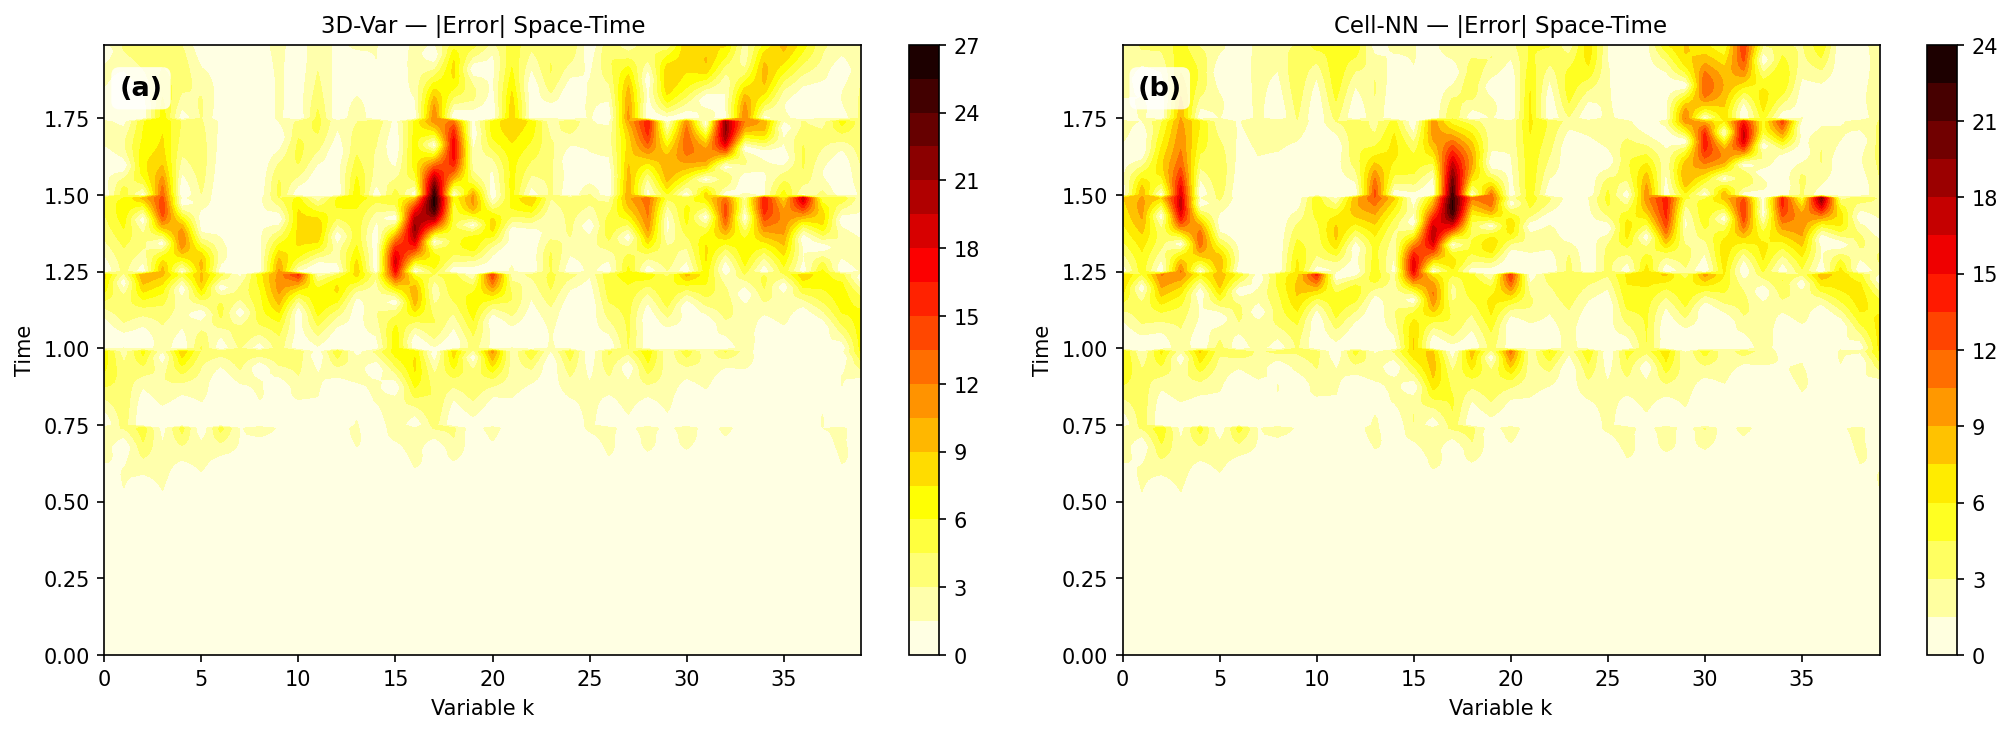
\includegraphics[width=\textwidth]{Figures/Supplementary/supplementary_fig1_error_spacetime.png}
\caption{Lorenz-96 DA error space-time diagrams: absolute error
$|X_\text{true}(k,t) - \hat{X}(k,t)|$ as a function of state variable
$k$ and time $t$. (a) 3D-Var, (b) Cell-NN, both corresponding
to the same realization shown in Figure~\ref{fig:lorenz96_da}.}
\label{fig:supp1}
\end{figure*}

\begin{figure*}[h]
\centering
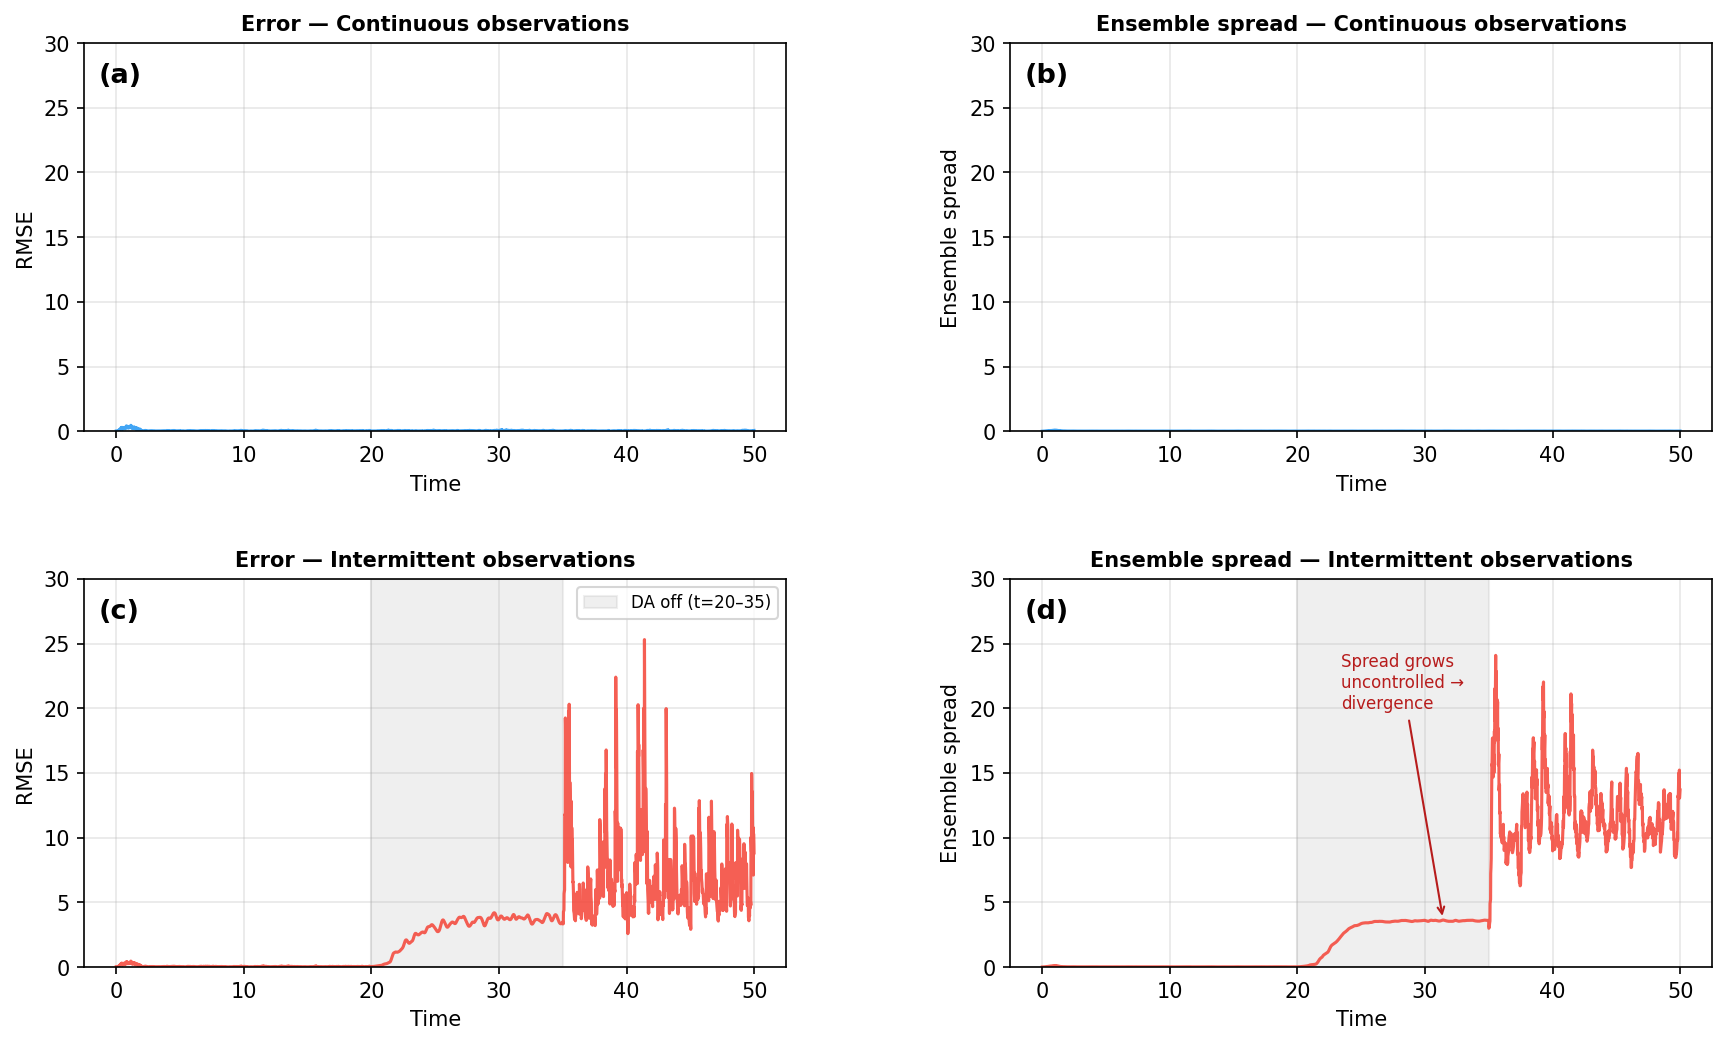
\includegraphics[width=\textwidth]{Figures/Supplementary/enkf_spread_diagnostic.png}
\caption{EnKF spread diagnostic: (a) ensemble error and (b) ensemble
spread under continuous observation availability; (c) ensemble error
and (d) ensemble spread under intermittent observation availability.
Grey shading marks the DA-off period. Spread grows 165-fold during
the gap (from 0.022 to 3.63) and reaches 4.22 when observations
resume.}
\label{fig:enkf_spread}
\end{figure*}

\renewcommand{\thetable}{S\arabic{table}}
\setcounter{table}{0}

\begin{table*}[h]
\centering
\caption{Seasonal breakdown of internal reconstruction validation
(test subset, $\kappa=0.4$, $n=50$). Coverage refers to mean fraction
of valid MODIS ocean pixels per composite in each season (land
excluded). BG = persistence background; Recon = Cell-NN
reconstruction.}
\label{tab:seasonal}
\begin{tabular}{lccccc}
\toprule
Season & $n$ timesteps & Coverage (\%) & BG RMSE & Reconstructed RMSE & Improvement \\
\midrule
SW Monsoon (Jun--Sep) & 80 & 29.6 & 0.9308 & 0.1614 & 82.7\% \\
NE Monsoon (Oct--Jan) & 74 & 70.6 & 0.6918 & 0.1265 & 81.7\% \\
Pre/Post-monsoon (Feb--May) & 75 & 63.9 & 0.6293 & 0.1091 & 82.7\% \\
\midrule
Overall & 229 & 54.1 & 0.7548 & 0.1330 & 82.4\% \\
\bottomrule
\end{tabular}
\end{table*}

\begin{figure*}[h]
\centering
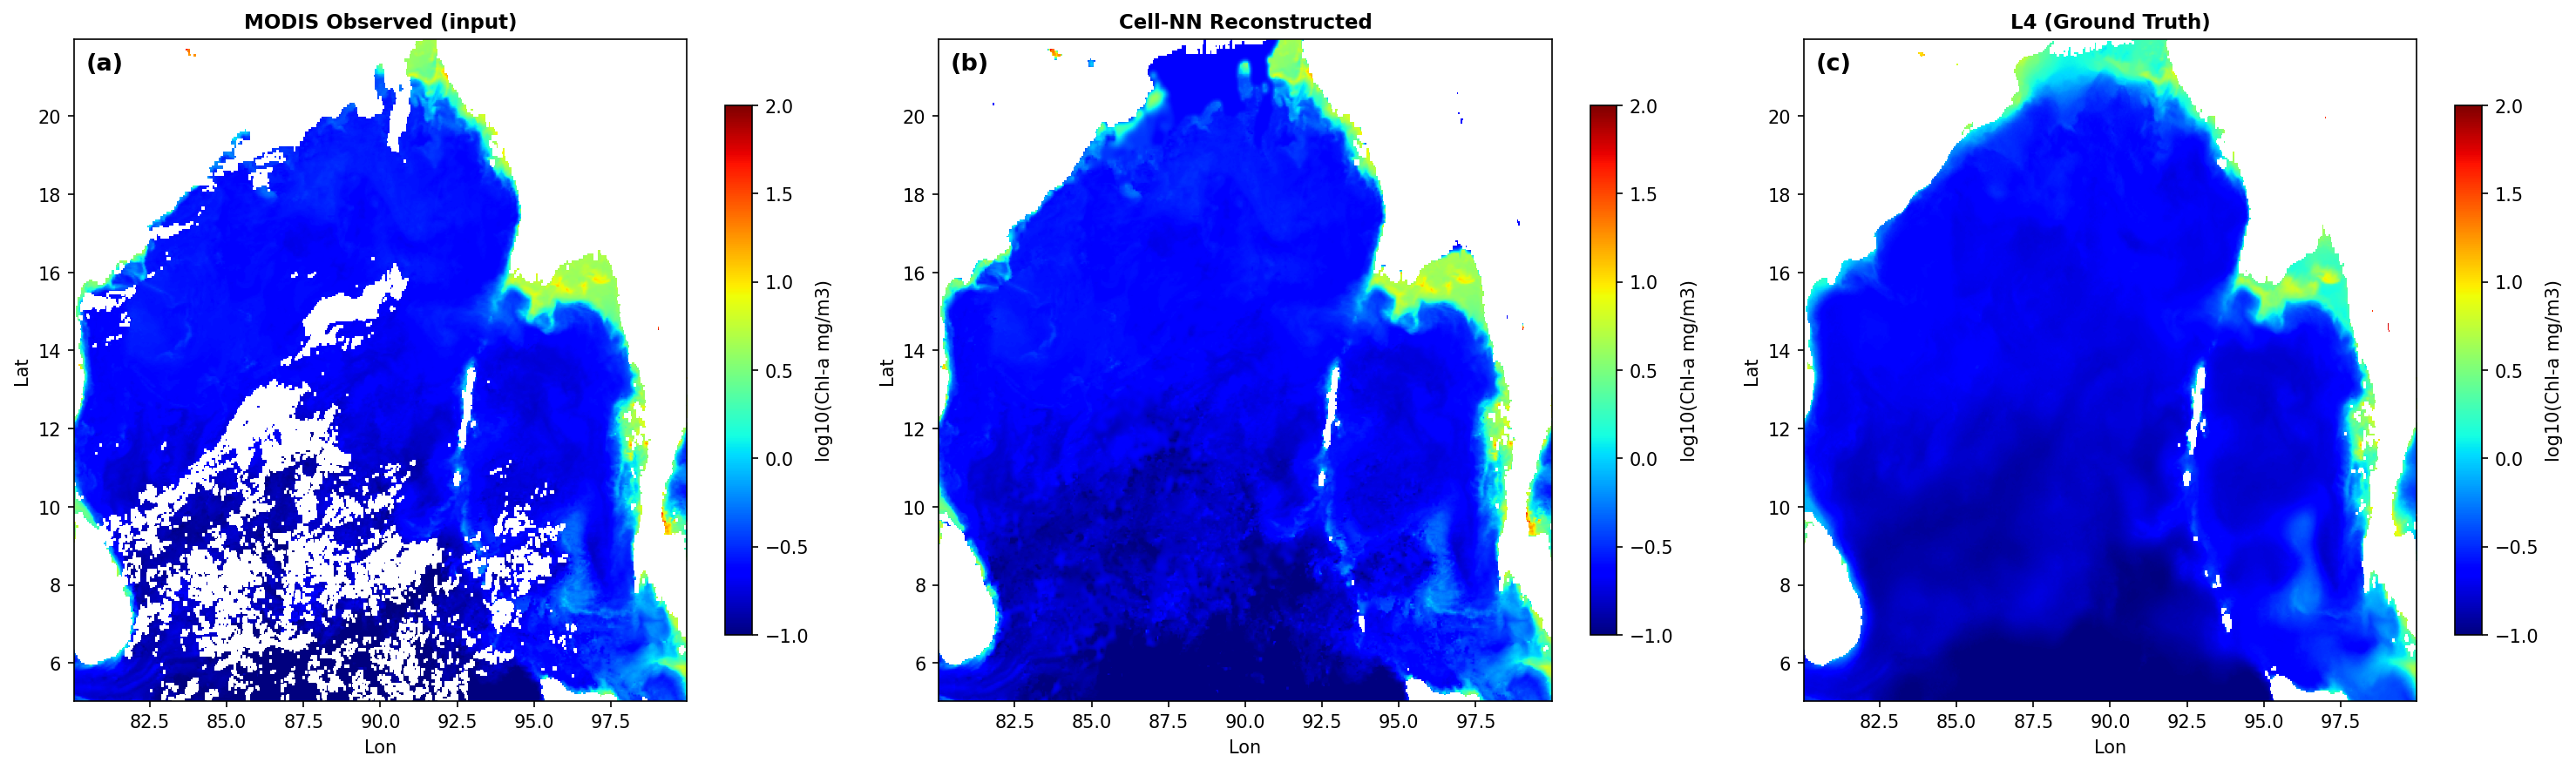
\includegraphics[width=\textwidth]{Figures/spatial_snapshot_jan2016.png}
\caption{Spatial snapshot comparison, 1 January 2016: (a) MODIS
observed input (63.4\% valid coverage), (b) Cell-NN reconstruction
(100\% ocean coverage, gap-filled), and (c) the independent L4
reference field, used here as ground truth. Panel (b)'s smoother
open-ocean texture, relative to panel (a), illustrates at a single
date the same low-pass smoothing documented statistically across the
full record in Section~\ref{sec:trend}.}
\label{fig:snapshot}
\end{figure*}

\begin{table}[h]
\centering
\small
\caption{Ablation: adding a fixed climatology-pull term to Cell-NN's
fallback for unobserved pixels, test subset (MC = Monte-Carlo).}
\label{tab:ablation}
\begin{tabular}{lccc}
\toprule
Anomaly bin & Cell-NN & +climatology & MC \\
\midrule
Typical    & 0.1068 & 0.0686 & 0.0911 \\
Moderate   & 0.1094 & 0.1150 & 0.1003 \\
Anomalous  & 0.1548 & 0.3028 & 0.1487 \\
Overall    & 0.1256 & 0.1912 & 0.1161 \\
\bottomrule
\end{tabular}
\end{table}
\end{document}